%%%%%%%%%%%%%%%%%%%%%%%%%%%%%%%%%%%%%%%%%%%%%%%%%%%%%%%%%%%%%%%%%%%%%%%%%%%%%%%
% This template is distributed with ABSOLUTELY NO WARRANTY.
% It serves as a guideline and constitutes a basic structure for a
% thesis/dissertation. The user assumes full responsibility for formatting
% and typesetting their document and for verifying that all the thesis
% requirements set by the University of Tennessee are met. Please refer to the most
% recent UT thesis guide (http://web.utk.edu/~thesis/thesisresources.shtml)
% or contact the thesis consultant (http://web.utk.edu/~thesis/).
% Please report any bugs to the thesis consultant.
%%%%%%%%%%%%%%%%%%%%%%%%%%%%%%%%%%%%%%%%%%%%%%%%%%%%%%%%%%%%%%%%%%%%%%%%%%%%%%%
% O P T I O N S:
% 1. thesis/dissertation
% 2. monochrome
% 3. all options provided by the report class
\documentclass[thesis,letterpaper,12pt]{utthesis} % thesis, one side
%%%%%%%%%%%%%%%%%%%%%%%%%%%%%%%%%%%%%%%%%%%%%%%%%%%%%%%%%%%%%%%%%%%%%%%%%%%
%                                                                         %
%                                 PREAMBLE                                %
%                                                                         %
%%%%%%%%%%%%%%%%%%%%%%%%%%%%%%%%%%%%%%%%%%%%%%%%%%%%%%%%%%%%%%%%%%%%%%%%%%%

%% LANGUAGE and ENDCODING
\usepackage[english]{babel}
\usepackage{lipsum}
\usepackage[utf8]{inputenc}
\usepackage[T1]{fontenc}

%% PACKAGES
\usepackage[section]{placeins}
\usepackage[usenames,dvipsnames]{xcolor}
\usepackage{microtype}
\usepackage[obeyDraft]{todonotes}
\usepackage{fancyvrb}
\VerbatimFootnotes
\usepackage{algorithmic}
\usepackage{booktabs}
\usepackage{tabularx}
\usepackage{multirow}
\usepackage{longtable}

%% GRAPHICS RELATED
\usepackage{graphicx}
\usepackage[outdir=./tmp/]{epstopdf}
\DeclareGraphicsExtensions{.eps, .pdf, .jpeg, .png}

%% ALGORTHIM
\usepackage[chapter]{algorithm}
\usepackage{algorithmic}

%% CPATION SETUP
\usepackage{float}
\usepackage{caption}
\usepackage{subcaption}
\captionsetup{belowskip=12pt,aboveskip=4pt}

%% UNITS,  EQUATIONS, and CHEMISTRY
\usepackage{textcomp}
\usepackage{siunitx}
\usepackage[version=3]{mhchem}
\usepackage{mathrsfs}

%% NOMENCLATURE
\usepackage[refpage]{nomencl}  % refer to the page where notation appears
\newcommand{\definevar}[2]{#1 is the #2\nomenclature{#1}{#2}}
\newcommand{\nom}[2]{#1 #2\nomenclature{#1}{#2}}
\renewcommand{\nomname}{List of Notations}
\renewcommand*{\pagedeclaration}[1]{\unskip\dotfill\hyperpage{#1}}
\makenomenclature
%%%%%%%%%%%%%%%%%%%%%%%%%%%%%%%%%%%%%%%%%%%%%%%%%%%%%%%%%%%%%%%%%%%%%%%%%%%
%                                                                         %
%                             Listing Setup                               %
%                                                                         %
%%%%%%%%%%%%%%%%%%%%%%%%%%%%%%%%%%%%%%%%%%%%%%%%%%%%%%%%%%%%%%%%%%%%%%%%%%%
\usepackage{listings}
\lstset{ %
    language=C++,
    basicstyle=\footnotesize\ttfamily,
    numbers=left,
    numberstyle=\tiny\color{gray},
    stepnumber=2,
    numbersep=5pt,
    backgroundcolor=\color{white},
    showspaces=false,
    showstringspaces=false,
    showtabs=false,
    frame=single,
    rulecolor=\color{black},
    tabsize=2,
    breaklines=true,
    breakatwhitespace=false,
    title=\lstname,
    keywordstyle=\color{blue},
    commentstyle=\color{OliveGreen},
    stringstyle=\color{orange}
}
\DeclareCaptionFont{white}{\color{white}}
\DeclareCaptionFormat{listing}{\colorbox[cmyk]{0.43, 0.35, 0.35, 0.01}{\parbox{\dimexpr\textwidth-2\fboxsep\relax}{#1#2#3}}}
\captionsetup[lstlisting]{format=listing,labelfont=white,textfont=white,singlelinecheck=false,margin=0pt,font={bf,footnotesize}}

%% USER COMMANDS
\usepackage{isotope}
\newcommand{\iso}{\isotope}
\newcommand{\figurewidth}{\textwidth}
\DeclareSIUnit\roetgen{R}
\DeclareSIUnit\eV{\electronVolt}
\DeclareSIUnit\count{count}
\DeclareSIUnit\rem{rem}
\DeclareSIUnit\in{in}
\DeclareSIUnit\cps{\count\per\second}
\DeclareSIUnit\cpsngcf{\count\per\second\per\nano\gram\iso[252]{Cf}}

%% Table of Contents
\addto\captionsenglish{%
 \renewcommand{\contentsname}{Table of Contents}%
}

% some alternatives are:
%\documentclass[thesis,monochrome,letterpaper,12pt]{utthesis} %thesis, one side, monochrome text
%\documentclass[thesis,twoside,letterpaper,12pt]{utthesis} % thesis, two side
%\documentclass[thesis,monochrome,twoside,letterpaper,12pt]{utthesis} % thesis, two side, monochrome text
% for a dissertation, replace the thesis option by dissertation:
% \documentclass[dissertation,letterpaper,12pt]{utthesis} . . .
\renewcommand{\baselinestretch}{1.5} 	 % line Spacing
%%%%%%%%%%%%%%%%%%%%%%%%%%%%%%%%%%%%%%%%%%%%%%%%%%%%%%%%%%%%%%%%%%%%%%%%%%%%%%%
% TO DO: FILL IN YOUR INFORMATION BELOW - READ THIS SECTION CAREFULLY
%%%%%%%%%%%%%%%%%%%%%%%%%%%%%%%%%%%%%%%%%%%%%%%%%%%%%%%%%%%%%%%%%%%%%%%%%%%%%%%
\title{Optimization of the Radiation Portal Monitor}
\author{Matthew J. Urffer}
\date{\today}
\copyrightYear{2013} 
\graduationMonth{December}
\majorProfessor{Liaurence F. Miller}
\keywords{Neutron Detectors, Radiation Portal Monitors, GEANT4, MCNPX, Simulation}
\college{Engineering}
\dept{Nuclear Engineering}
\university{The University  of Tennessee, Knoxville}
\viceProvost{Carolyn R. Hodges}
\major{Nuclear Engineering}
\degree{Doctor of Philosophy}
\college{Engineering}
\dept{Nuclear Engineering}
\university{The University  of Tennessee, Knoxville}
\numberOfCommitteeMembers{3}
\committeeMemberA {Lawrence H. Heilbronn}
\committeeMemberB {Dayaker Penumadu}
\committeeMemberC {Ronald E. Pevey}
%%%%%%%%%%%%%%%%%%%%%%%%%%%%%%%%%%%%%%%%%%%%%%%%%%%%%%%%%%%%%%%%%%%%%%%%%%%%%%%
% LOAD SOME USEFUL PACKAGES
%%%%%%%%%%%%%%%%%%%%%%%%%%%%%%%%%%%%%%%%%%%%%%%%%%%%%%%%%%%%%%%%%%%%%%%%%%%%%%%
\graphicspath{{tmp/}{figures/}{figures/eps/}{figures/pdf/} }% specify the path where figures are located
\usepackage{fancyhdr}                   % fancy headers and footers
\usepackage[inactive]{srcltx}		 	% necessary to use forward and inverse searching in DVI
\usepackage{relsize}                    % font sizing hierarchy
%%%%%%%%%%%%%%%%%%%%%%%%%%%%%%%%%%%%%%%%%%%%%%%%%%%%%%%%%%%%%%%%%%%%%%%%%%%%%%%
\begin{document}
    \pagenumbering{alph} % this is needed to clear certain issues with the hyperref package
    %
    %
    \addToPDFBookmarks{0}{Front Matter}{rootNode} % create a root node named "Front Matter" in the pdf bookmarks
    \addToPDFBookmarks{1}{Title}{a} % add a pdf bookmark to the title page
    \maketitle
    %
    \pagenumbering{roman}
    \setcounter{page}{2}
    %
    \addToPDFBookmarks{1}{Dedication}{b} % add a pdf bookmark to the dedication page
    \chapter*{}
\begin{center}
{\centering \textit{To my family and friends}}
\vspace{2 cm}
\begin{figure}[h]
\centering

\includegraphics[width=0.5\textwidth]{tryScience}
\end{figure}
\end{center} 

 % include the dedication
    %
    \addToPDFBookmarks{1}{Acknowledgements}{c} % add a pdf bookmark to the acknowledgements page
    \chapter*{Acknowledgments}

This works would not have been possible without the support of many different people.
Dr. Miller has been an essential resource for bouncing ideas around while providing valuable insights and supporting this work.
I would also like to thank my committee members, Dr. Heilbronn, Dr. Penumadu, and Dr. Pevey, for their support and technical expertise that they have provided. 
The testing of films would not have been possible without the kind folks fabricating the materials, I would like to acknowledge the work of Dr. Mabe, Dr. Auxier II, and Dr. Uppal for their help and numerous conversations.

The academic portion of this would would have never succeeded without the support from my friends and family. 
My mother and father, Lisa and Micheal, deserve special recognition of their support, encouragement and frank advice. 
Katie, Samuel, David, Isaac, Esther and Eli also deserve recognition for their support and efforts. 
Finally, I would like to thank the members of Knoxville Ultimate for being supportive and offering many great games.
 % include the acknowledgements
    \addToPDFBookmarks{1}{Abstract}{d} % add a pdf bookmark to the title page
    \begin{abstract}
    \chapter*{Abstract}
\label{chap:abstract}
Alternative neutron detection technologies are required to replace the current He-3 based Radiation Portal Monitors (RPM) which are employed to detect special nuclear material that may be entering the United States illicitly.
Replacement technologies must fulfill the following criteria established by the Department of Homeland Security: 1) a neutron detection efficiency, 2) a gamma insensitivity, and 3) the performance of the detector should not suffer in the the presence of a strong gamma field.
Polymeric films containing Li-6 ranging from 15 to 300 microns have the ability to fulfill these criteria if suitably utilized.
For a typical detector material the design involves maximizing the neutron-gamma discrimination, maximizing the physical detector configuration in order to ensure optimal use of the incident neutron spectra, and ensuring that the scintillation light generated can be collected.

A technique for using a pulse height discriminator for rejecting gamma interactions has been determined for polymeric films  ranging from 15 microns to 300 microns in thickness.
The basis of this technique has been attributed to the relative ranges of the secondary electrons of the Compton scattered electrons (generally in the hundred of keV) from the gamma interactions, compared to the ranges of the electrons from the reaction products of a neutron absorption, which have energies int he 10 keV range.
Detailed Monte Carlo simulations indicate that a desired film thickness is around 100 microns.

A replacement portal monitor has been designed for layered polymeric films that effectively utilize enriched Li-6 in the detector material using a genetic algorithm to optimize the spacing between the layers, while cylindrical designs could also be employed.
If two photomultiplier tubes are placed at the top and bottom of a fishtail light guide mounted on the top and bottom of the detector cabinet, eight precent of the optical photons generated in a 10 precent loaded polystyrene film can be collected, leaving an acceptable number of photons to create a signal.

    \end{abstract}
    %
    \pagenumbering{roman}
    \setcounter{page}{2}
    %
    \addToPDFBookmarks{1}{Table of Contents}{e}
    \tableofcontents % generate a table of contents
    %
    \addToPDFBookmarks{1}{List of Tables}{f}
    \listoftables % generate a list of tables
    %
    \addToPDFBookmarks{1}{List of Figures}{g}
    \listoffigures % generate a list of figures
    %
    \makenomenclature % OPTIONAL
    \addToPDFBookmarks{1}{Nomenclature}{h} % OPTIONAL
    \printnomenclature[1.25in] % OPTIONAL
    %
    \newpage
    \pagenumbering{arabic}
    \setcounter{page}{1}
    %%%%%%%%%%%%%%%%%%%%%%%%%%%%%%%%%%%%%%%%%%%%%%%%%%%%%%%%%%%%%%%%%%%%%%%%%%%
    % INCLUDE THE CHAPTERS STARTING WITH THE NOMENCLATURE IF PRESENT
    %%%%%%%%%%%%%%%%%%%%%%%%%%%%%%%%%%%%%%%%%%%%%%%%%%%%%%%%%%%%%%%%%%%%%%%%%%%
    %%%%%%%%%%%%%%%%%%%%%%%%%%%%%%%%%%%%%%%%%%%%%%%%%%%%%%%%%%%%%%%%%%%%%%%%%%%
%                                                                         %
%                         PROJECT INTRODUCTION                            %
%                                                                         %
%%%%%%%%%%%%%%%%%%%%%%%%%%%%%%%%%%%%%%%%%%%%%%%%%%%%%%%%%%%%%%%%%%%%%%%%%%%
\chapter{Introduction} 
\label{chap:Intro}
Radiation Portal Monitors (RPMs) are passive radiation detection systems implemented at over a thousand of border crossings, designed to determine if cargo contains any special nuclear material in a safe, nondestructive, and effective manner\cite{kouzes_neutron_2010}. 
However, the current technology used in RPMs for detecting neutrons emitted from special nuclear material use a rapidly diminishing resource, \iso[3]{He}, that cannot be economically replaced. 
The Department of Homeland Security (DHS) continues to fund research (through the Domestic Nuclear Detection Office (DNDO)) for the development of detector systems to detect radioactive material that could potentially be used to cause significant economic loss and loss of life.  
As a result of this research a number of alternative detection systems continue to be investigated with the most viable including: boron trifluoride filled proportional detectors, boron-lined proportional detectors, \iso[6]{Li} loaded scintillation glass fiber detectors, and \iso[6]{Li} plus scintillator-coated wavelength-shifting fiber detectors\cite{pnnl_18471,kouzes_neutron_2010}.  

Neutron detectors often utilize a material with a large cross section for absorption, such as \iso[6]{Li} or \iso[10]{B}.
When these materials absorb a neutron they usually disintegrate to produce ionized reaction products that in turn transfer their kinetic energy to electrons.
In the case of the $\iso[6]{Li}\left(n,\iso[3]{H}\right)\alpha$ reaction, the fission energy is distributed between a triton of energy \SI{2.73}{\mega\eV} and an alpha of energy \SI{2.05}{\mega\eV}.
In a proportional counter such as the \iso[3]{He} based detectors,the energy from the charged particles would ionize a gas, creating a voltage signal.
Scintillator detectors, on which this work is based, utilize the charged particle energy depositions to create electron excitations in the scintillating material which are then transfered by fluors and produce visible light, which is detected with a photomultiplier tube.

\section{Replacement Detector Criteria}
\label{sec:ReplacmentCriteria}
Pacific Northwest National Lab (PNNL) along with the DNDO have developed a set of specifications that that replacement RPMs must meet \cite{kouzes_neutron_2010, kouzes_neutron_1999}. 
In particular 1) an absolute neutron detection efficiency greater than \SI{2.5}{\cps\per\ng \iso[252]{Cf}} at \SI{2}{\meter} for a defined moderated  source, 2) an intrinsic gamma-neutron detection efficiency of one in a million, and 3) a gamma absolute rejection ratio for neutrons stating that the performance of the detector should not change by more than 10\% in a \SI{10}{\milli\roetgen\per\hour} gamma field.
These parameters are summarized in \autoref{tab:DHSCritera}.
\begin{table}
  \centering
	\caption{Replacement Portal Monitor Criteria}
	\begin{tabular}{m{8cm} m{6cm} }
	Parameter & Specification \\
	\hline
	\hline
	Absolute neutron detection efficiency & 2.5 cps/ng of \iso[252]{Cf} (in specified test configuration) \\
	Intrinsic gamma-neutron detection efficiency & $ \epsilon_{int,\gamma n}\leq 10^{-6}$ \\
	Gamma absolute rejection ratio for neutrons (GARRn) & $ 0.9 \leq \text{ GARRn }\leq$ 1.1 at 10 mR/h exposure \\
	Cost &  \$ 30,000 per system \\
	\end{tabular}
	\label{tab:DHSCritera}
\end{table}

The absolute neutron detection efficiency $\left (\epsilon_{abs,n} \right )$ is defined as the number of neutron pulses recorded by the detector normalized by the number of neutrons emitted by the source as shown in \autoref{eqn:absn}
\begin{align}
	\label{eqn:absn}
  \epsilon_{abs,n} = \frac{N_{nc}}{N_{ns}}
\end{align}
where \definevar{$N_{nc}$}{neutron count rate} and \definevar{$N_{ns}$}{neutron emission rate from the source}.
DNDO guidelines state that a \iso[252]{Cf} source placed \SI{2}{\meter} from the midpoint of the detector is to be used for the determination of the absolute neutron detection efficiency\cite{pnnl_18471}.
To reduce the gamma ray flux of \iso[252]{Cf} upon a candidate detector the source is shielded by at least \SI{0.5}{\cm} of lead, and the neutron spectrum is then moderated by \SI{2.5}{\cm} of polyethylene\cite{pnnl_18471}.
The intrinsic efficiency, which provides a measure of how sensitive the detector is to incoming radiation, is defined in \eqref{eqn:inteff}.
\begin{align}
  \label{eqn:inteff}
  \epsilon_{int} = \frac{\text{Number Counts Observed}}{\text{Number Quanta for Radiation Crossing Detector}}
\end{align}
The formulation presented in \eqref{eqn:inteff} is then adapted to photons, with the requirement that only one count per a million photons passing through the detector may be registered.
To account for this the subscript $\gamma n$ is added to the intrinsic efficiency \eqref{eqn:inteffNG}
\begin{align}
  \label{eqn:inteffNG}
  \epsilon_{int,\gamma n} &= \frac{P_{pc}}{P_{p\Phi}}
\end{align}
where \definevar{$P_{pc}$}{photon count rate} and \definevar{$P_{p\Phi}$}{photons crossing the detector}.
The intrinsic gamma-neutron detection efficiency is to be measured using either a \iso[192]{Ir}, \iso[137]{Cs}, or \iso[60]{Co} source placed at an appropriate distance so as to produce an exposure rate of \SI{10}{\milli\roetgen\per\hour} at the detector\cite{kouzes_neutron_1999}.
The final detector parameter, the gamma absolute rejection ratio (GARRn), characterizes the detector response in the presence of both a large gamma ray source (\SI{10}{\milli\roetgen\per\hour}) and a \iso[252]{Cf} neutron source (configured as it would be for an absolute neutron detection efficiency measurement).
This criteria, shown in \eqref{eqn:garrn}, implies that the performance of the detector should not change by more than 10\% in a strong gamma field\cite{kouzes_neutron_1999}.
\begin{align}
  \label{eqn:garrn}
  GARRn = \frac{ \epsilon_{abs,\gamma n}}{\epsilon_{abs,n}}
\end{align}

%%%%%%%%%%%%%%%%%%%%%%%%%%%%%%%%%%%%%%%%%%%%%%%%%%%%%%%%%%%%%%%%%%%%%%%%%%%
%                                                                         %
%                       CURRENT TECHNOLOGIES                              %
%                                                                         %
%%%%%%%%%%%%%%%%%%%%%%%%%%%%%%%%%%%%%%%%%%%%%%%%%%%%%%%%%%%%%%%%%%%%%%%%%%%
\section{Current Technologies}
\label{sec:CurrentTechnologies}
Currently a number of alternative technologies is being developed, but two of the most promising detector technologies are boron loaded straw fibers being developed by Proportional Technologies Inc. (Houston, TX) and LiF loaded ZnS(Ag) scintillator paddles being developed by Innovative American Technology (Coconut Creek, FL).
The boron straw tubes meet the count rate criteria with a gamma rejection rate estimated at \num{4e-9} while passing the GARRn \cite{kouzes_boron-lined_2012}.
LiF/ZnS(Ag) is a commercial inorganic scintillator that utilizes the alpha from the \iso[6]{Li} neutron capture to active the ZnS doped with silver (ZnS(Ag)). 
LiF/ZnS(Ag) has a high light output per neutron (\num{1.6E5} photons per neutron) with a decay time of approximately \SI{100}{\micro\second} and the maximum emission at \SI{450}{\nm} \cite{carel_w.e_inorganic-scintillator_2001}.
However, this material is opaque and therefore care needs to be taken with the light collection of a large area detector.
Innovative American Technology (IAT) has developed a design of a replacement RPM that utilizes LiF/ZnS(Ag), as shown schematically in \autoref{fig:IATRender} and in \autoref{fig:IATImage}.
Current testing indicates that this detector design will meet the DHS criteria\cite{kouzes_lithium_2010}.
\begin{figure}
  \centering
  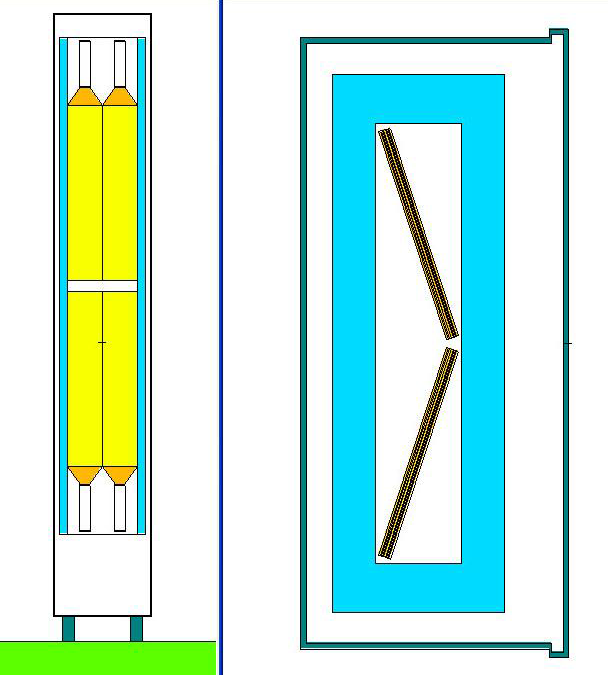
\includegraphics[width=0.5\textwidth]{IATRender}
	\caption[Rendering of IAT Neutron Detector]{Modeled IAT detector that consist of four paddles.  The paddles are angled to expose a larger surface to the neutron flux\cite{pnnl_22228}.}
	\label{fig:IATRender}
\end{figure}
\begin{figure}
  \centering
  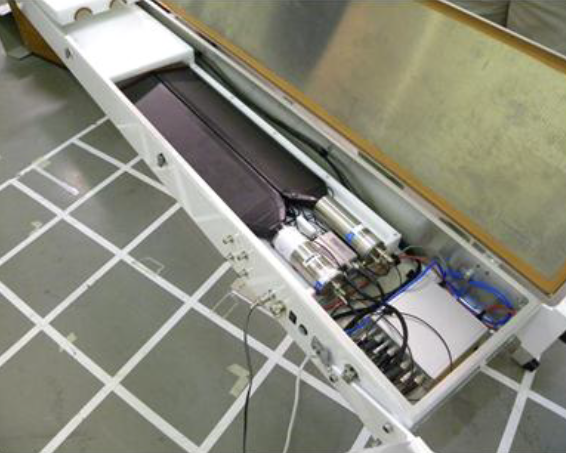
\includegraphics[width=0.75\textwidth]{IATImage}
	\caption[Photograph of IAT Neutron Detector]{Photograph of the developed IAT detector\cite{pnnl_22228}.}
	\label{fig:IATImage}
\end{figure}

%%%%%%%%%%%%%%%%%%%%%%%%%%%%%%%%%%%%%%%%%%%%%%%%%%%%%%%%%%%%%%%%%%%%%%%%%%%
%                                                                         %
%                       DEVELOPED SCINTILLATORS                           %
%                                                                         %
%%%%%%%%%%%%%%%%%%%%%%%%%%%%%%%%%%%%%%%%%%%%%%%%%%%%%%%%%%%%%%%%%%%%%%%%%%%
\section{Developed Scintillators}
\label{sec:DevelopedScintillators}
In addition to the inorganic scintillator LiF/ZnS(Ag), work is being completed at the University of Tennessee to construct thin film polymeric scintillators to be utilized in a layered detector design for replacement RPMs.
These films, either based on polystyrene (PS) or polyethylene naphthalate (PEN), are \iso[6]{LiF} containing polymers projected to be low cost, have high mechanical durability, and meet the detector criteria \cite{Sen_Composites,Mabe201329}.
The developed materials have been characterized for their neutron performance and gamma discrimination abilities, a summary of which (as of May 2013) may be found in \autoref{chap:MeasuredFilmPerfomance}.
%%%%%%%%%%%%%%%%%%%%%%%%%%%%%%%%%%%%%%%%%%%%%%%%%%%%%%%%%%%%%%%%%%%%%%%%%%%
%                                                                         %
%                       OPTIMIZATION INTRODUCTION                         %
%                                                                         %
%%%%%%%%%%%%%%%%%%%%%%%%%%%%%%%%%%%%%%%%%%%%%%%%%%%%%%%%%%%%%%%%%%%%%%%%%%%
\section{Optimization Opportunities}
There exists a need to build predictive modeling capabilities of these detectors in order to optimize the detector performance.
For a particular material and neutron absorber the detector geometry can be optimized to maximize the energy deposited in scintillation material by charged particles relative to the energy deposited by photon interactions. 
This in turn permits one to maximize the recorded neutron interaction rate relative to recorded photon interaction rates by setting a lower level discriminator (LLD) above a threshold associated with energy deposited in the detector by photons.  
As the LLD is increased, the efficiency for detecting neutrons is diminished; however, the intrinsic efficiency for detecting neutrons relative to photons is dramatically increased. 
In addition, as the neutron flux is being moderated and absorbed by the RPM material there exist the opportunity to position the neutron absorber films to maximize the neutron count rate while minimizing the amount of material being used.
Finally, it is essential to ensure that the scintillation light can be collected efficiency.

%%%%%%%%%%%%%%%%%%%%%%%%%%%%%%%%%%%%%%%%%%%%%%%%%%%%%%%%%%%%%%%%%%%%%%%%%%%
%                                                                         %
%                       ORGINAL CONTRIBUTION                              %
%                                                                         %
%%%%%%%%%%%%%%%%%%%%%%%%%%%%%%%%%%%%%%%%%%%%%%%%%%%%%%%%%%%%%%%%%%%%%%%%%%%
\section{Original Contribution}
\label{sec:OrginalContribution}
The design of effective radiation portal monitors is a critical component in detecting and subsequent interdiction of special nuclear material.
Most researchers assume that adequate neutron-gamma discrimination can be achieved by the relatively low mass attenuation coefficient for polymers and taking advantage of the thinness of a detector, but for a common plastic based scintillator the detector would have to be less than \SI{160}{\nm} in order to have an interaction rate less than one in a million.
This work is unique in that the fundamental physics basis of the neutron-gamma discrimination is not attributed to the mass attenuation coefficient but rather to the ranges of the secondary electrons from photon interactions in the material depositing less energy than their neutron counterparts.
Current modeling work in large area neutron detectors focuses either with monolithic plastic slab geometries or with neutronic calculations that do account for light collection and transport.
A layered detector design, while not unique, has not been optimized using a genetic algorithm for which the formulation or the problem is quite natural.
In addition, little modeling work has been completed on the performance of a radiation portal monitor including light transport, which is a large majority of this work.


%%%%%%%%%%%%%%%%%%%%%%%%%%%%%%%%%%%%%%%%%%%%%%%%%%%%%%%%%%%%%%%%%%%%%%%%%%%
%                                                                         %
%                               DOCUMENT LAYOUT                           %
%                                                                         %
%%%%%%%%%%%%%%%%%%%%%%%%%%%%%%%%%%%%%%%%%%%%%%%%%%%%%%%%%%%%%%%%%%%%%%%%%%%
\section{Organization of Disseration}
The layout of this document follows the optimization of the design from the detector material to the optimal placement of the material.
\autoref{chap:SecElectron} describes the measurements and simulations preformed in order to determine the the optimal thickness for a single film.
\autoref{chap:GARPMOpt} provides an overview of the various designs that could be considered to utilize the detector material, and then a layered detector design is optimized with the use of a genetic algorithm.
The detector design is finalized in \autoref{chap:LightTransport} where light transport is employed to determine if the detector design would be feasible given a films measured performance.
Finally, \autoref{chap:Conclusions} serves to summarize the various lessons of the detector design.
  % Problem introduction
    \chapter{Neutron - Gamma Discrimination}
\label{chap:SecElectron}

Effective neutron-gamma discrimination is integral to the performance of the detector.
Generally, two methods are available for discrimination; 1) pulse shape discrimination and 2) pulse height discrimination.
In pulse shape discrimination the different decay times between the neutron and gamma pulses are exploited to develop a metric that allows for the classification of the pulse.
Generally, pulse shape discrimination works best when the pulses are noticeably different.
Pulse height discrimination is based on setting a pulse height discriminator that acts as a partition between two classes of pulses.
This is generally easier to implement than pulse shape discrimination.
While some of the fabricated films show a small basis for pulse shape discrimination, this work will only focus on pulse height discrimination.

The pulse height discriminator setting necessary to achieve the neutron-gamma discrimination is achieved through the use of a mathematical lower level discriminator (MLLD).
This virtual discriminator establishes the bound where $\epsilon_{int,\gamma n}\leq 10^{-6}$, and counts above the MLLD are classified as neutron counts. 

It is currently understood that the light output per path length of the film (which is directly proportional to the pulses collected on the PMT) is related to the stopping power of the radiation in the film material.
For a given material the stopping power of the film will be constant, and therefore the light output of the film can be found by integrating the light output per path length over the total length of the film.
It is then possible to conclude that the light output of a film is proportional to the energy deposited in the film.

Preferential energy deposition by neutrons relative to gammas will enhance the discrimination by creating larger neutron light pulses than the gamma pulses, allowing for fewer neutron pulses to be classified as gamma pulses because they are below the MLLD.
Thus, neutron-gamma discrimination can be enhanced by optimizing the energy deposition in the film. 

The organization of this chapter is as follows.
An overview of scintillation mechanics of organic scintillators will be provided in \autoref{sec:ScintMechanics} in order to understand the relationship between scintillation and the energy deposited by charged particles.
The energy spectra and ranges of neutron and gamma reaction products will be discussed in \autoref{sec:InteractionsAndRange} (focusing on polystyrene) to explain the basis for the difference in energy depositions. 
Calculations of the energy deposition will be shown in \autoref{sec:EnergyDep} for polymeric materials, providing the foundation of neutron-gamma pulse height discrimination.

%%%%%%%%%%%%%%%%%%%%%%%%%%%%%%%%%%%%%%%%%%%%%%%%%%%%%%%%%%%%%%%%%%%%%%%%%%%
%                                                                         %
%                      SCINTILLATION MECHANICS                            %
%                                                                         %
%%%%%%%%%%%%%%%%%%%%%%%%%%%%%%%%%%%%%%%%%%%%%%%%%%%%%%%%%%%%%%%%%%%%%%%%%%%
\section{Scintillation Mechanisms}
\label{sec:ScintMechanics}
%%%%%%%%%%%%%%%%%%%%%%%%%%%%%%%%%%%%%%%%%%%%%%%%%%%%%%%%%%%%%%%%%%%%%%%%%%%
%                                                                         %
%                         Introduction to Scintillation                   %
%                                                                         %
%%%%%%%%%%%%%%%%%%%%%%%%%%%%%%%%%%%%%%%%%%%%%%%%%%%%%%%%%%%%%%%%%%%%%%%%%%%
Scintillation detecctors (the detectors on which this work is based) utilize a scintillator to convert ionizing radiation into photons, and then transporting and capturing those the emitted photons, commonly with a photomultiplier tube (PMT).
The electrical signal from the PMT is then an indicator of a radiation event in the detector's scintillator material.
The current RPM's with \iso[3]{He} are ion chamber detectors, however, the proposed \iso[6]{Li} glass detectors and \iso[6]{LiF} doped ZnS:Ag detectors are scintillation based detectors. 

\subsection{Organic Scintillators}
An organic scintillator generally has a $\pi$-electron structure, as shown in \autoref{fig:pielectron}.
An incoming particle (generally electrons liberated from the energy deposition of the ionizing radiaiton) then excites one of the modes of the $\pi$-electron structure.
Higher singlet states rapidly (on the order of picoseconds) relax to the first singlet state, and excessive vibrational energy (populations of the vibrational sates) is lost.
Thus, after a short period of time the entire excitation population is in the $S_10$ state, and the decay of this state creates the prompt fluorescence.
\begin{figure}
  \centering
  \includegraphis[width=\textwidth]{PiElectronSates}
  \caption[$\pi$ Electron Structure]{Typicall $\pi$-electron structure of an organic molecule. The ground state of the molecule is shown as $S_0$, and excited single states are $S_1$, $S_2$ etc The triplet states are $T_1$, $T_2$, with the vibrational states as $S_OO$, $S_01$, $S_02$ and so forth. Figure from Wikipedia.}
  \label{fig:pielectron}
\end{figure}
The exictations of triplet states typically yield delayed scintillation events or phosphorescence.
An exicted triplet states immediately decays to the $T_0$ state by internal degration without a photon emission.
The $T_0$ state typically decays by interacting with another $T_0$ state in a $T_0 + T_0 \to S^* + S_0 + h\nu$ transition.
The excited singlet state $S^*$ then also decays to the $S_0$ state.
The $T_0 + T_0$ transitions is slower than direct singlet state dexcitations, and results in a slow component of the pulse, which can be used for pulse shape discrimination.

Several factors need to be considered in order of a material to be considred as a scintilaltor:
\begin{itemize}
  \item The light yield should be linearly proportional to the energy deposition
  \item The material should be optically transparent to it's own wavelength of emission
  \item A short rise time with a fast decay time
\end{itemize}
Scintillators convert the energy deposited in the material by ionizing radiation in to photons.



%%%%%%%%%%%%%%%%%%%%%%%%%%%%%%%%%%%%%%%%%%%%%%%%%%%%%%%%%%%%%%%%%%%%%%%%%%%
%                                                                         %
%                      ENERGY SCALE AND RANGES                            %
%                                                                         %
%%%%%%%%%%%%%%%%%%%%%%%%%%%%%%%%%%%%%%%%%%%%%%%%%%%%%%%%%%%%%%%%%%%%%%%%%%%
\section{Charged Particle Interactions and Ranges}
\label{sec:InteractionsAndRange}
%%%%%%%%%%%%%%%%%%%%%%%%%%%%%%%%%%%%%%%%%%%%%%%%%%%%%%%%%%%%%%%%%%%%%%%%%%%
%                                                                         %
%                      ENERGY SCALE AND RANGES                            %
%                                                                         %
%%%%%%%%%%%%%%%%%%%%%%%%%%%%%%%%%%%%%%%%%%%%%%%%%%%%%%%%%%%%%%%%%%%%%%%%%%%
The theoretical basis for the difference in energy deposition lies in the different mechanisms between charged particle interactions and photon interactions in matter.
For photons with energies between approximately \SI{0.5}{\MeV} and \SI{5}{\MeV} Compton scattering is the predominant interaction mechanism between the material and the photon.
The probability of an electron having a given kinetic energy after scattering can be expressed as \autoref{eqn:dSdEKlienNishina} (see \autoref{ch:ComptonScatter} for derivation details)
\begin{align}
  \label{eqn:dSdEKleinNishina}
\frac{d\sigma}{dE_e} = 2\pi r_e^2 \sin \theta f(\theta)\left [ \frac{1+\frac{E}{m_e c^2}\left(1-\cos\theta \right)^2}{E^2 \sin \theta} \right ]
\end{align}
provided  $f(\theta)$ is defined as $f(\theta) = \frac{1}{2}\left(\frac{E'}{E}\right)^2 \left(\frac{E'}{E} + \frac{E}{E'}-\sin^2\theta\right)$.
This distribution is shown for \iso[60]{Co} in \autoref{fig:Co60ComptonScatterSpectra}.
It is then highly likely that the Compton scattered electron will have an energy close to that of the maximum energy for the Compton scattering, \SI{0.96}{\MeV} for the \SI{1.173}{\MeV} photon and \SI{1.12}{\MeV} for the \SI{1.33}{\MeV} photon.
\begin{figure}
  \centering
  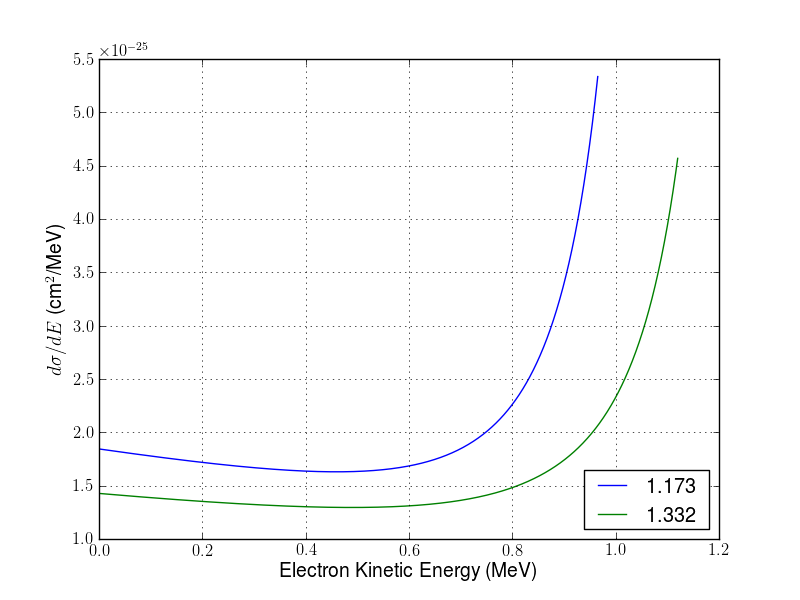
\includegraphics[width=\textwidth]{Co60ComptonScatteredSpectra}
  \caption[Gamma (Co-60) Compton Scattered Spectra]{Probability per energy of an Compton Scattered Electron having a given kinetic energy from \iso[60]{Co}}
  \label{fig:Co60ComptonScatterSpectra}
\end{figure}
The cumulative distribution function (CDF) is shown in \autoref{fig:Co60ComptonScatterCDF}.
\begin{figure}
  \centering
  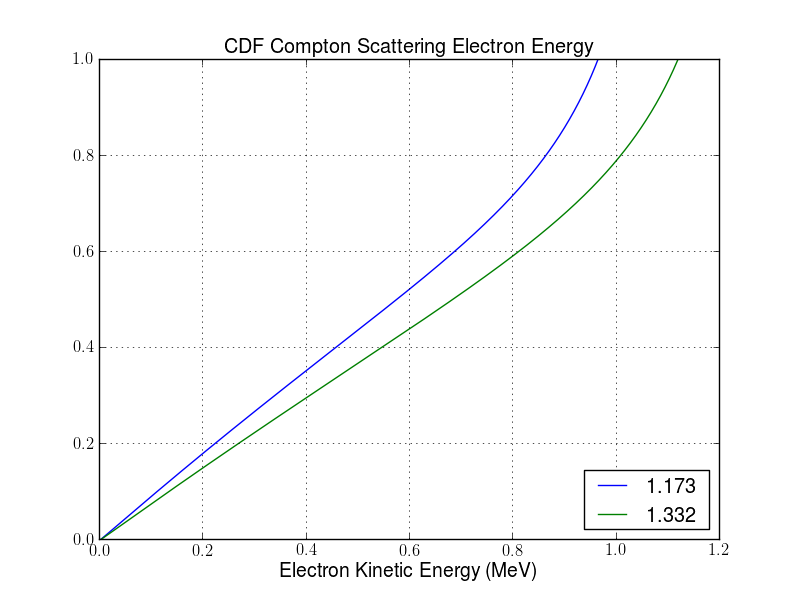
\includegraphics[width=\textwidth]{Co60ComptonScatteredSpectraCDF}
  \caption[Gamma (Co-60) Compton Scattered CDF]{Probability of the energy of a Compton Scattered Electron from \iso[60]{Co}. Over half of the electrons from the Compton scattering will have an energy greater than \SI{0.5}{\MeV}}
  \label{fig:Co60ComptonScatterCDF}
\end{figure}
In the case of $\iso[6]{Li}\left(n,\iso[3]{H}\right)\alpha$ the fission energy is distributed between a triton of energy \SI{2.73}{\mega\eV} and an alpha of energy \SI{2.05}{\mega\eV}.
The maximum kinetic energy of an electron from a Compton scattering event with an impingement \iso[60]{Co} source is \SI{1.117}{\mega\eV} (for the \SI{1.332}{\mega\eV} gamma). 
In polystyrene with a density of \SI{1}{\gram\per\cm\cubed}, the range of the maximum electron from Compton scattering is around \SI{4.5E3}{\um}\cite{berger_estar_2005}.
If elastic scattering between the alpha, triton and electrons is assumed the maximum kinetic energy of an electron is \SI{1.097}{\kilo\eV} for the alpha particle and \SI{1.986}{\kilo\eV} for the triton\cite{turner_atoms_2008}.
The range of the electron from a gamma interaction is more than \num{1E3} times greater than the range of electrons from an alpha or triton (Table \ref{tab:BasicEDepOutline}).
Therefore, it is more likely that the electrons generated by the alpha and the triton deposit significantly more of their energy in a thin film than the electron from a gamma.
This is also reflected in the stopping power, where the reaction product secondary electrons have a stopping power 40 times that of the secondary electrons from a gamma \cite{berger_estar_2005}.
The simulated electron range distributions for several energies is shown in \autoref{fig:ElectronRanges}.
\begin{table}[ht]
  \caption{Electron Energy, Range, and Stopping Power\protect\cite{berger_estar_2005,turner_atoms_2008}}
	\centering
	\begin{tabular}{c | c S c}
	{Electron Parent} & {Electron Energy} & {Total Stopping Power} & {CSDA Range} \\
	 &  & \si{\mega\eV \cm\squared \per \gram} & \si{\gram\per\cm\squared} \\
	\hline
	\hline
	{gamma}  & \SI{1.12}{\mega\eV} & 1.79 & $\ge$~\num{4.48E-1} \\
	{triton} & \SI{1.99}{\kilo\eV} & 75.1 & $\le$~\num{2.55E-4} \\
	{alpha}  & \SI{1.10}{\kilo\eV} & 113  & $\le$~\num{2.55E-4} \\
	\end{tabular}
  \label{tab:BasicEDepOutline}
	% See pg. 87 of Matthew's lab notebook for the calculation
\end{table}
\begin{figure}
  \centering
    \begin{subfigure}[b]{0.45\textwidth}
      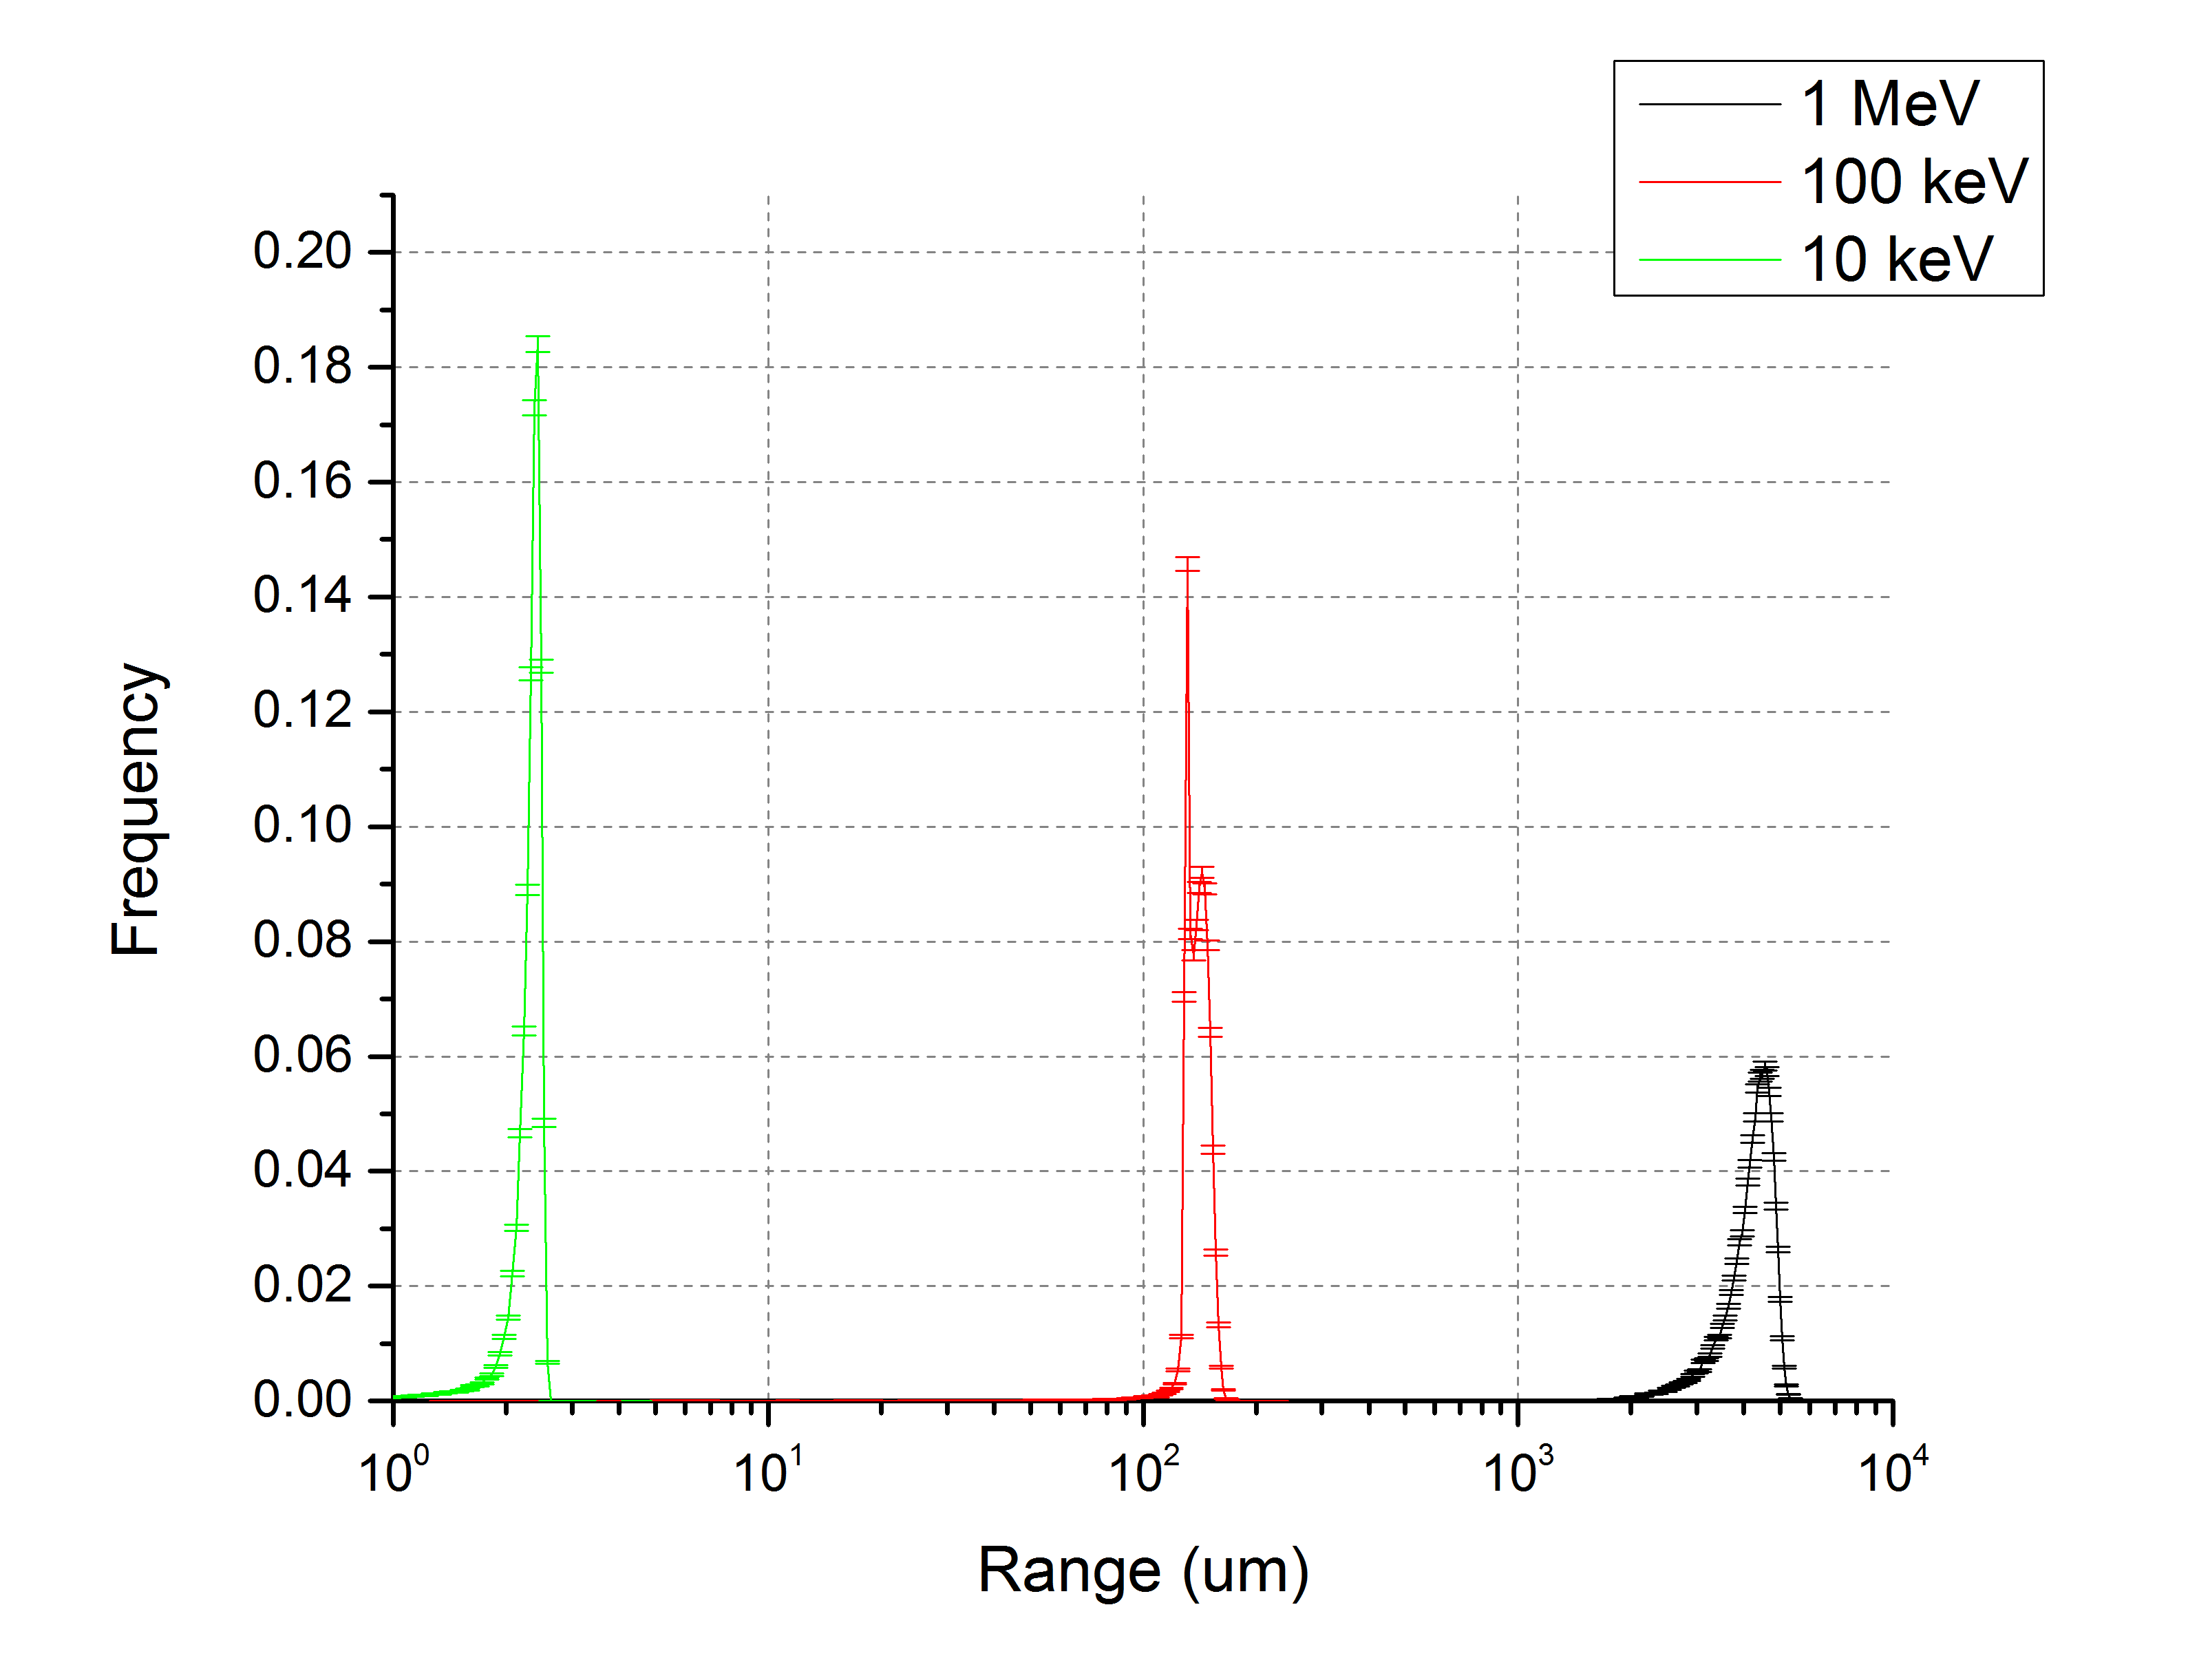
\includegraphics[width=\textwidth]{ElectronRangeDistribution}
      \caption[Range of \SI{1}{\MeV}, \SI{100}{\keV}, and \SI{10}{\keV} electrons]{Simulated ranges (GENAT4) of \SI{1}{\MeV}, \SI{100}{\keV}, and \SI{10}{\keV} electrons.}
    \end{subfigure}%
    ~
    \begin{subfigure}[b]{0.45\textwidth}
      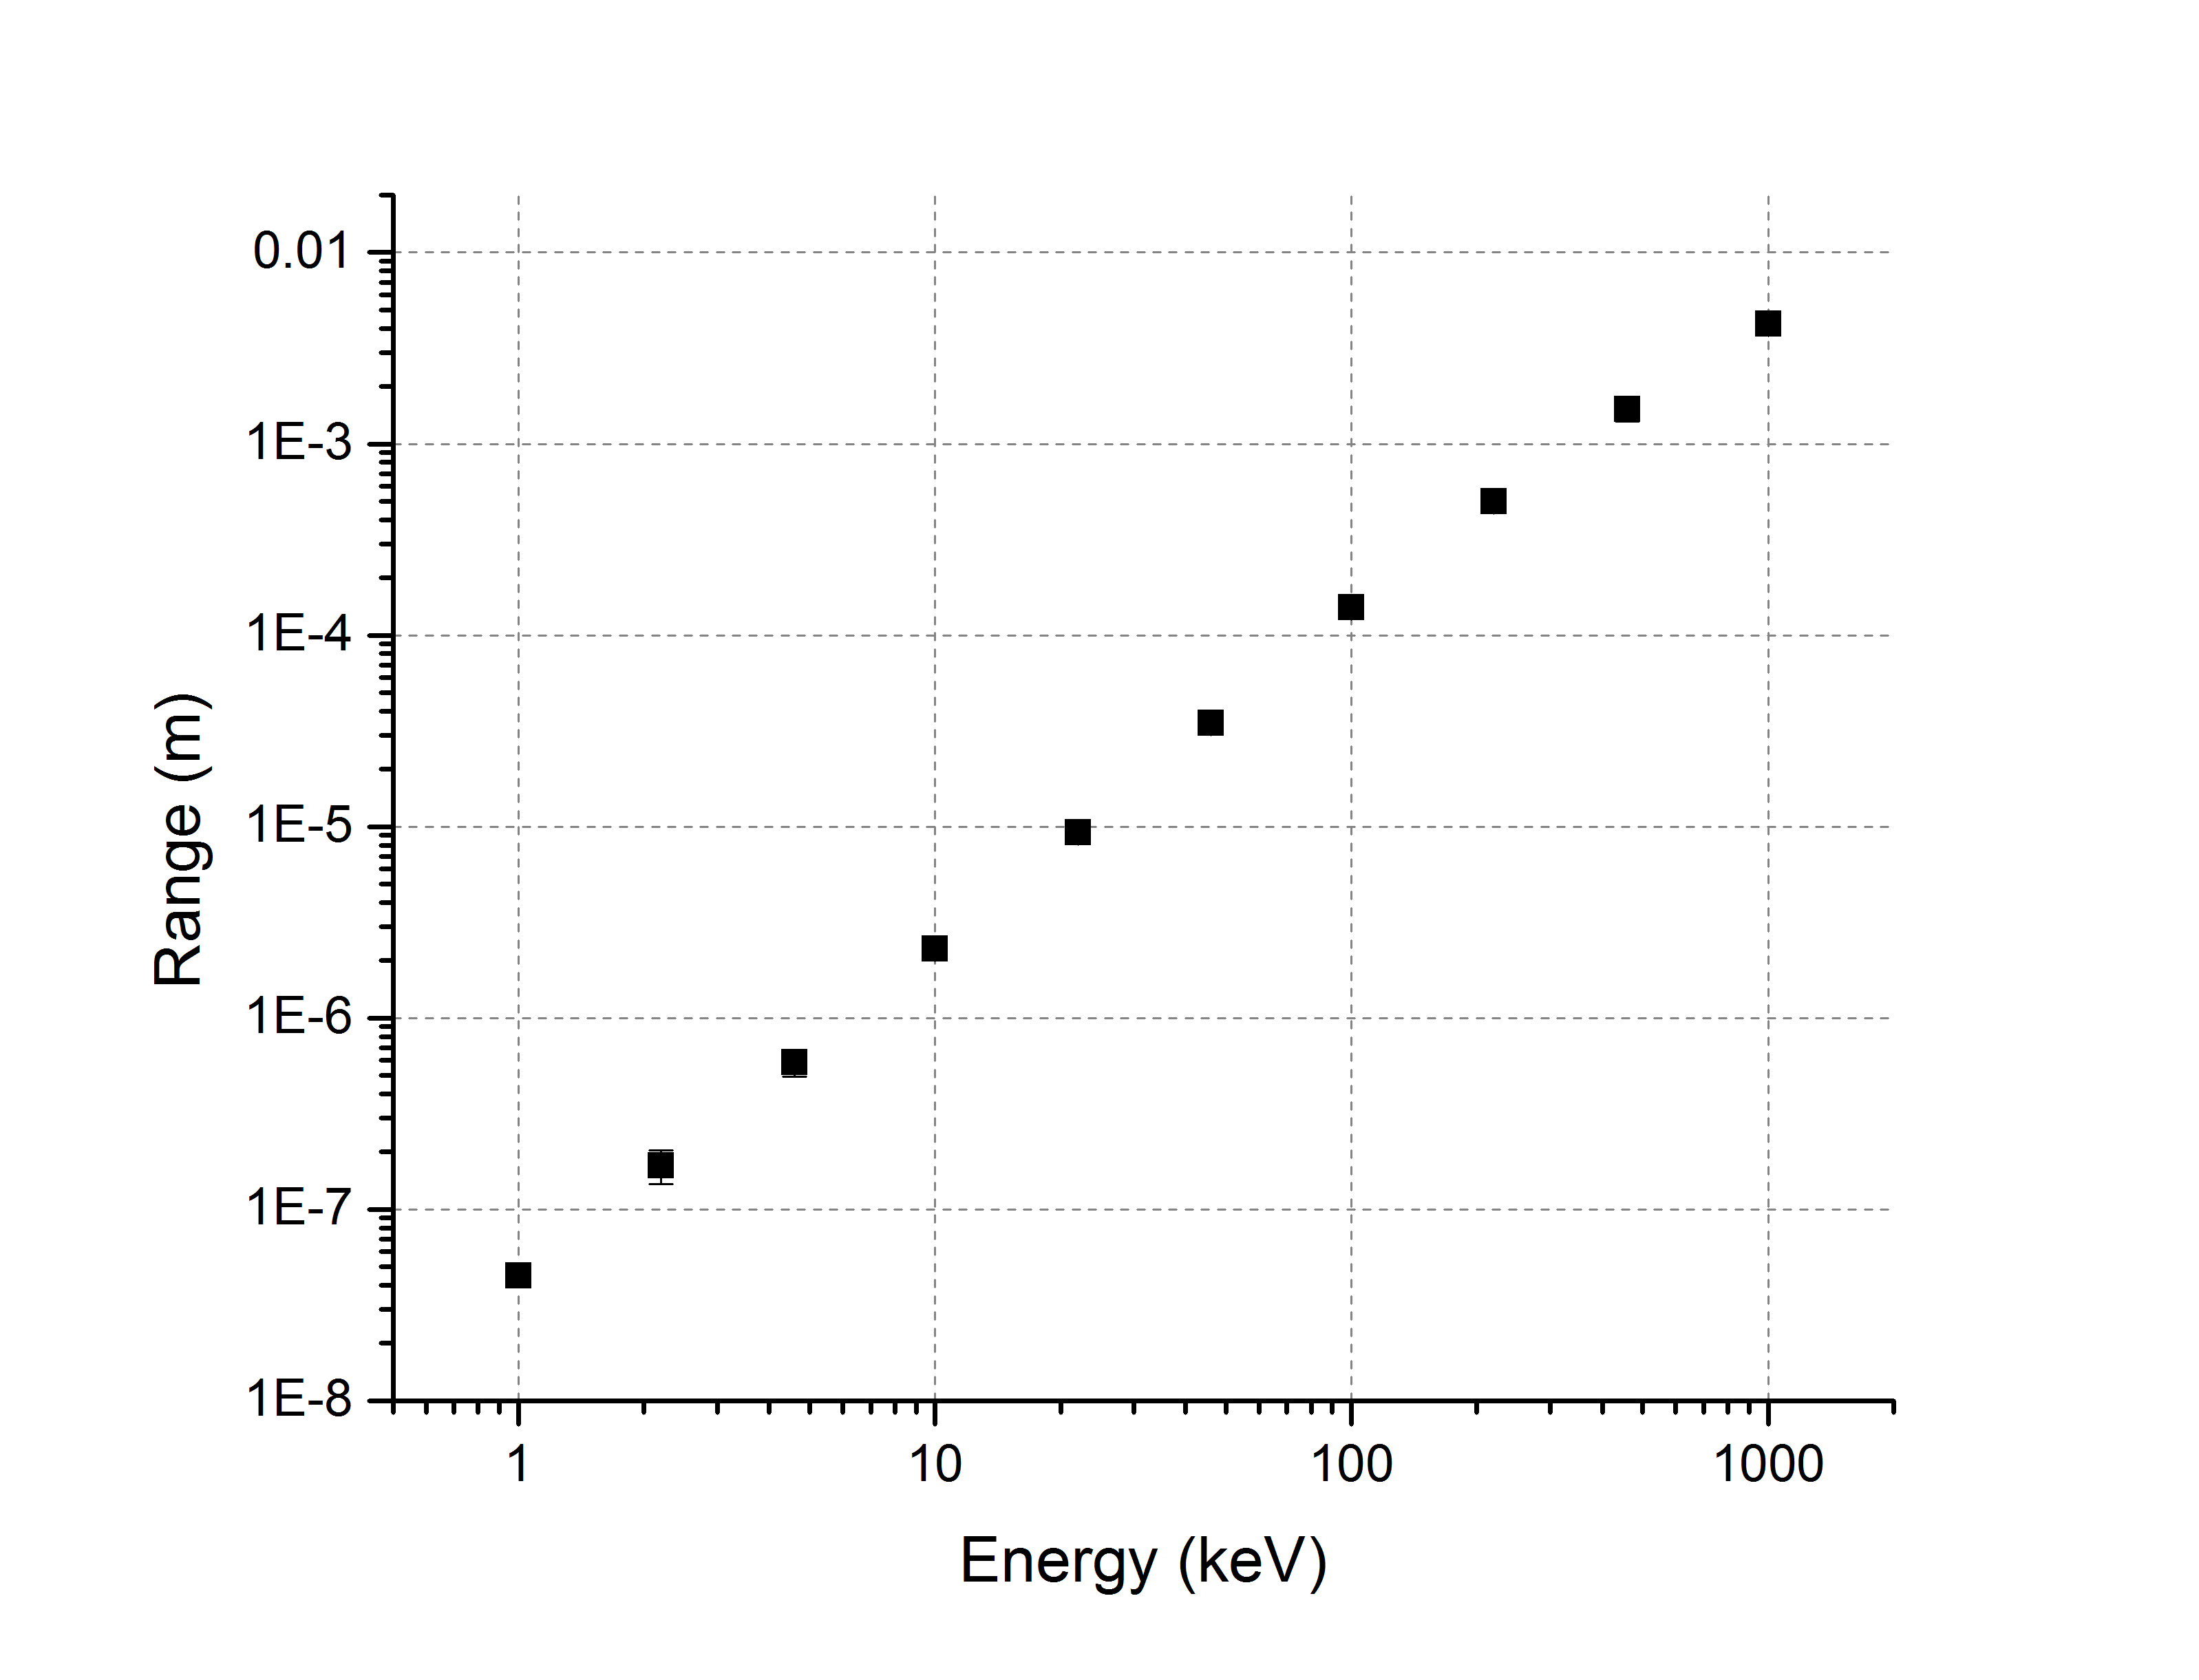
\includegraphics[width=\textwidth]{ElectronRange}
      \caption[Range of Electrons in Polystyrene]{Simulated (GEANT4) range of electrons in polystyrene. Compton scatted electrons from \iso[60]{Co} on the order of  \~ 100 keV will have ranges two orders of magnitude than that of electrons from the charged particle interactions.}
    \end{subfigure}
  \label{fig:ElectronRanges}
\end{figure}

The development of the secondary electron energy ranges so far has been from a simplified treatment of the problem when only the dominant process are considered.
Detailed simulations are necessary in order to have a greater understanding of the problem. 
The energy of the electrons created from an alpha (\SI{2.05}{\MeV}), triton (\SI{2.73}{\MeV}), and gammas from \iso[60]{Co} were calculated using a GEANT4 simulation, and overlaid on the range of electrons as shown in \autoref{fig:ERangeAndDist}.
It is then clear that the electrons from the \iso[60]{Co} will travel much father than those from the $\iso[6]{Li}\left(n,\alpha\right)\iso[3]{H}$ reaction products.
\begin{figure}
  \centering
  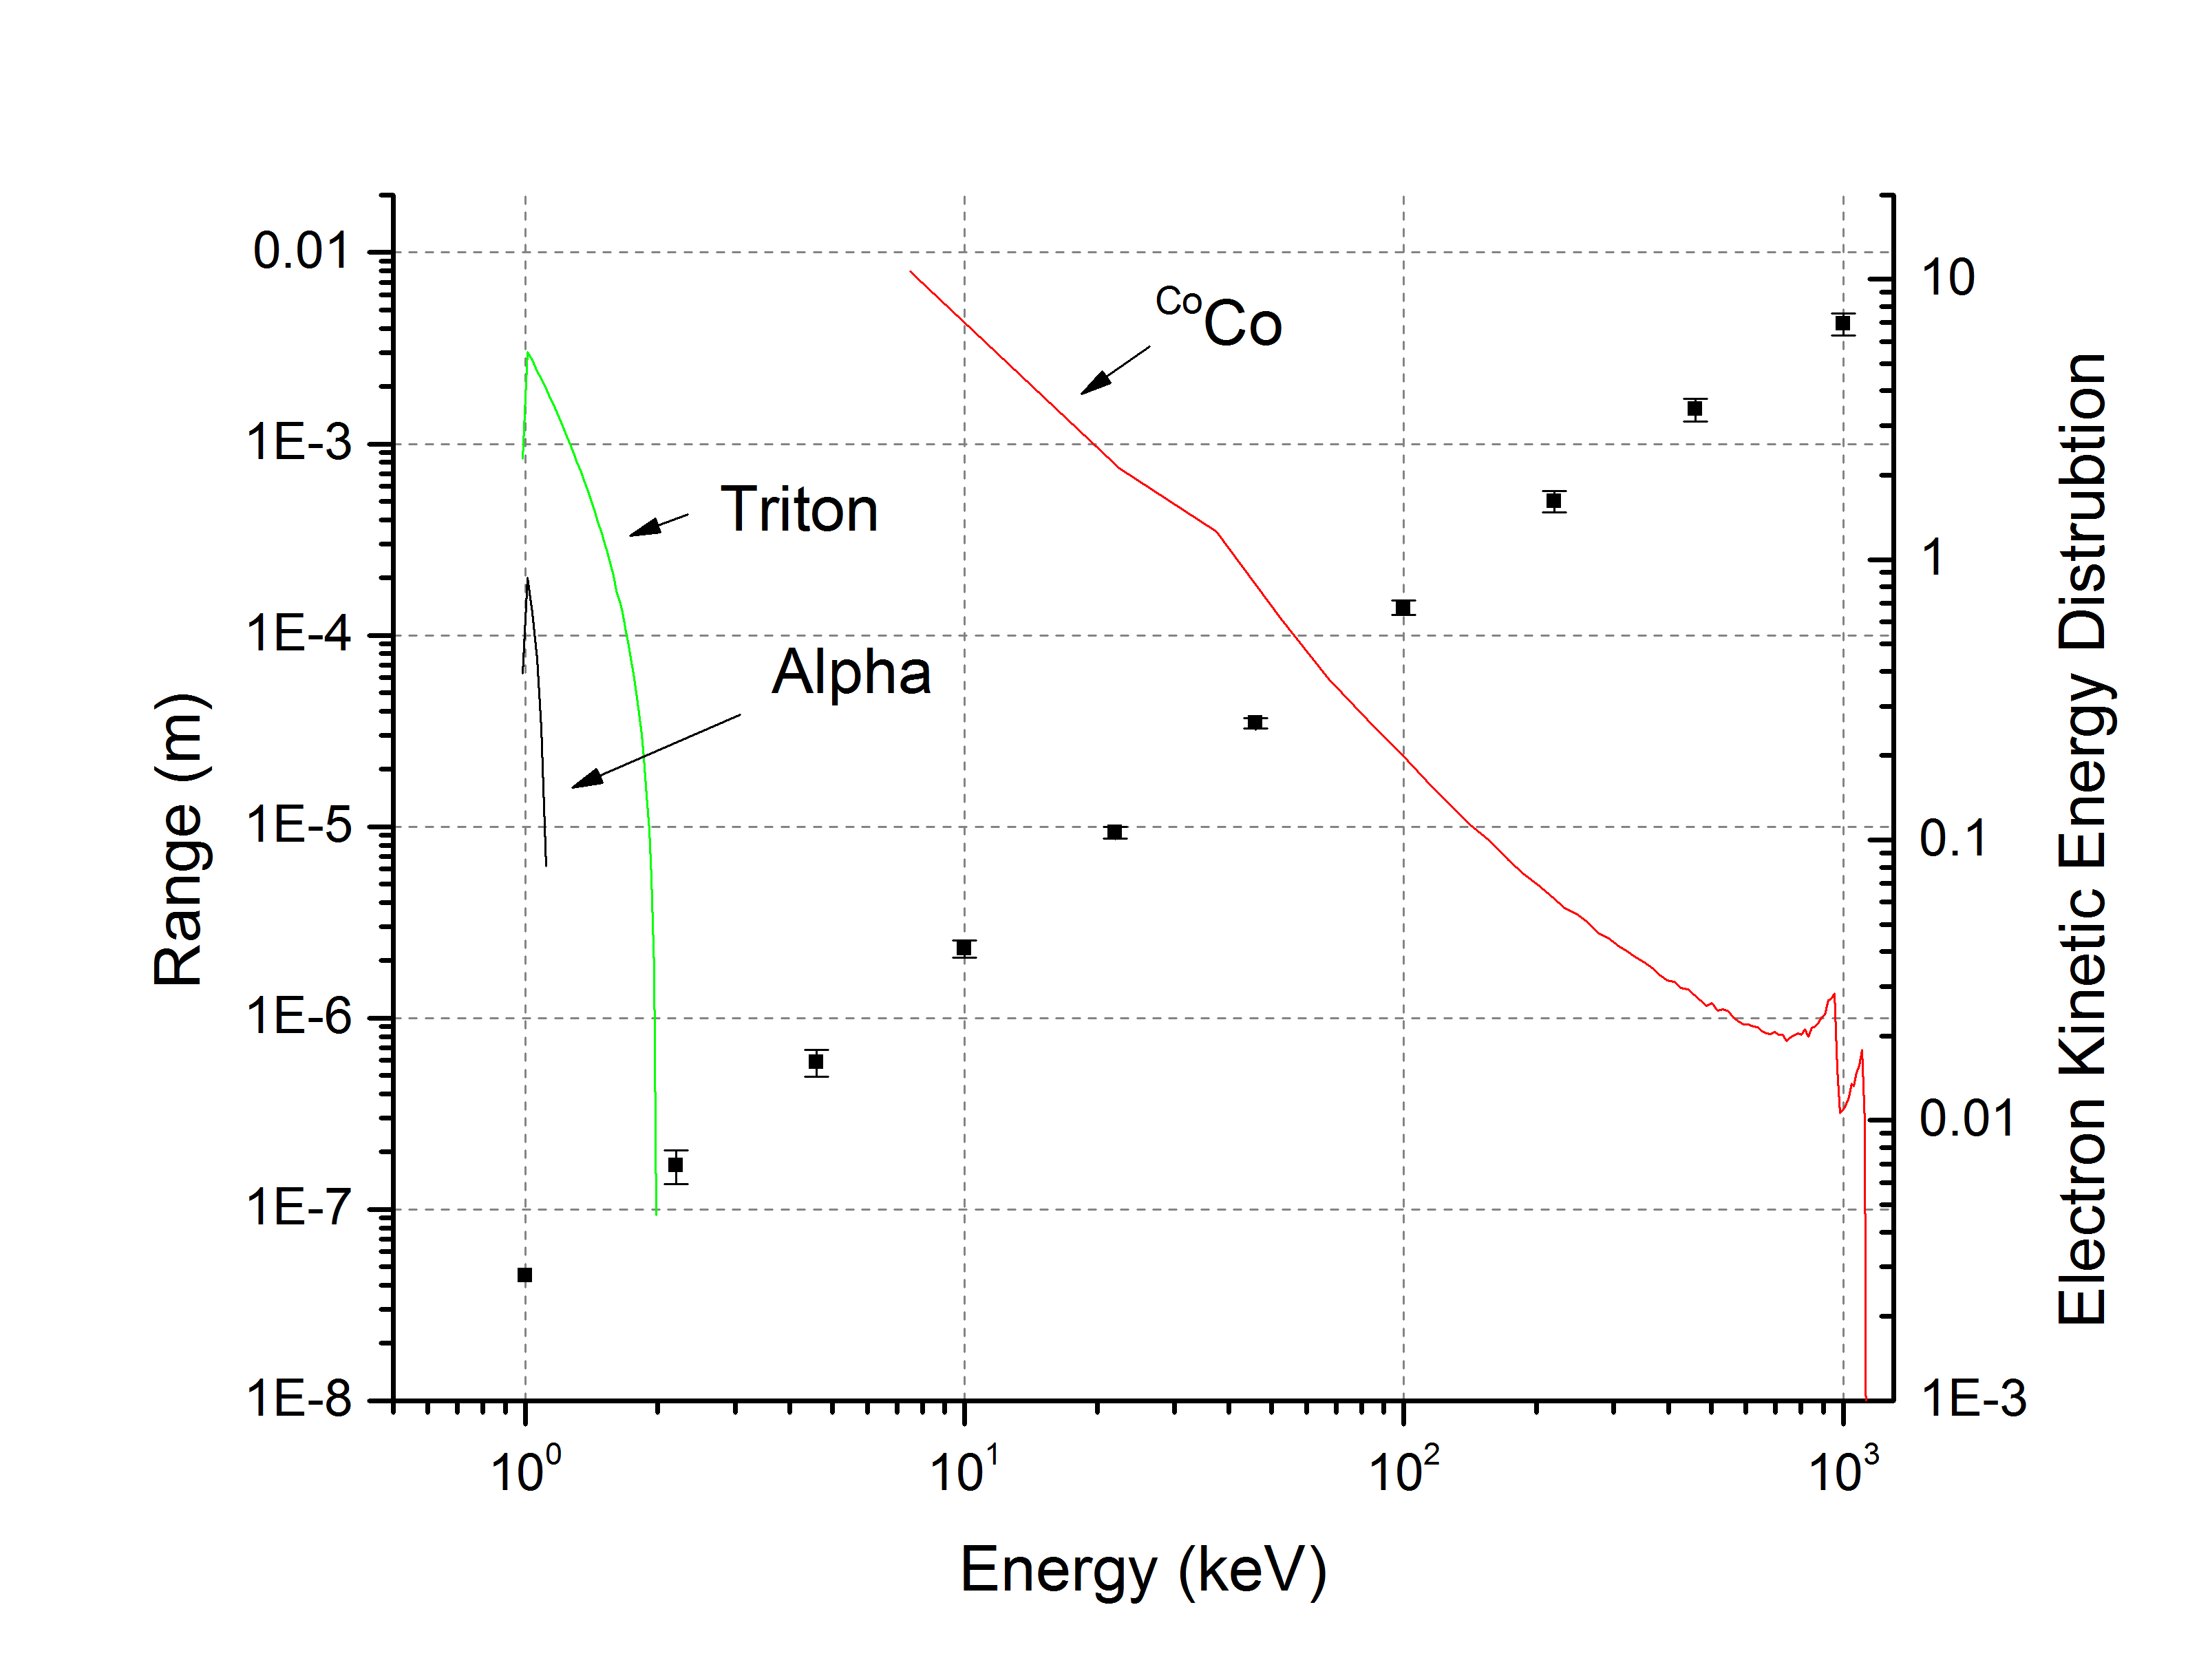
\includegraphics[width=\textwidth]{ElectronRangeAndEnergyDist}
  \caption[Electron Range and Energy Distribution of Selected Reactions]{The electron range (left axis) overlaid with the kinetic energy of electrons from \SI{2.05}{\MeV} alpha, \SI{2.73}{\MeV} triton, and gammas from \iso[60]{Co}. The \iso[60]{Co} electrons have energies much greater than the alpha and triton}
  \label{fig:ERangeAndDist}
\end{figure}

%%%%%%%%%%%%%%%%%%%%%%%%%%%%%%%%%%%%%%%%%%%%%%%%%%%%%%%%%%%%%%%%%%%%%%%%%%%
%                                                                         %
%                     ENERGY DEPOSITION SIMULATIONS                       %
%                                                                         %
%%%%%%%%%%%%%%%%%%%%%%%%%%%%%%%%%%%%%%%%%%%%%%%%%%%%%%%%%%%%%%%%%%%%%%%%%%%

\section{Energy Deposition Simulations}
\label{sec:EnergyDeposition}
The GEANT4 toolkit has the ability to track the energy deposition in different materials as well as the tracking of electrons to a least \SI{1}{\keV}\cite{agostinelli_geant4simulation_2003}.
It is proposed to represent the detector geometry as a single layer of neutron absorbing thin polymeric film mounted on top of a non-scintillating material (PMMA).
For simplicity, the initial events for runs will be chosen by setting up a particle gun for thermal (\SI{0.025}{\eV}) neutrons upon the detector and for both gammas resulting from a \iso[60]{Co} decay.
\begin{figure}
  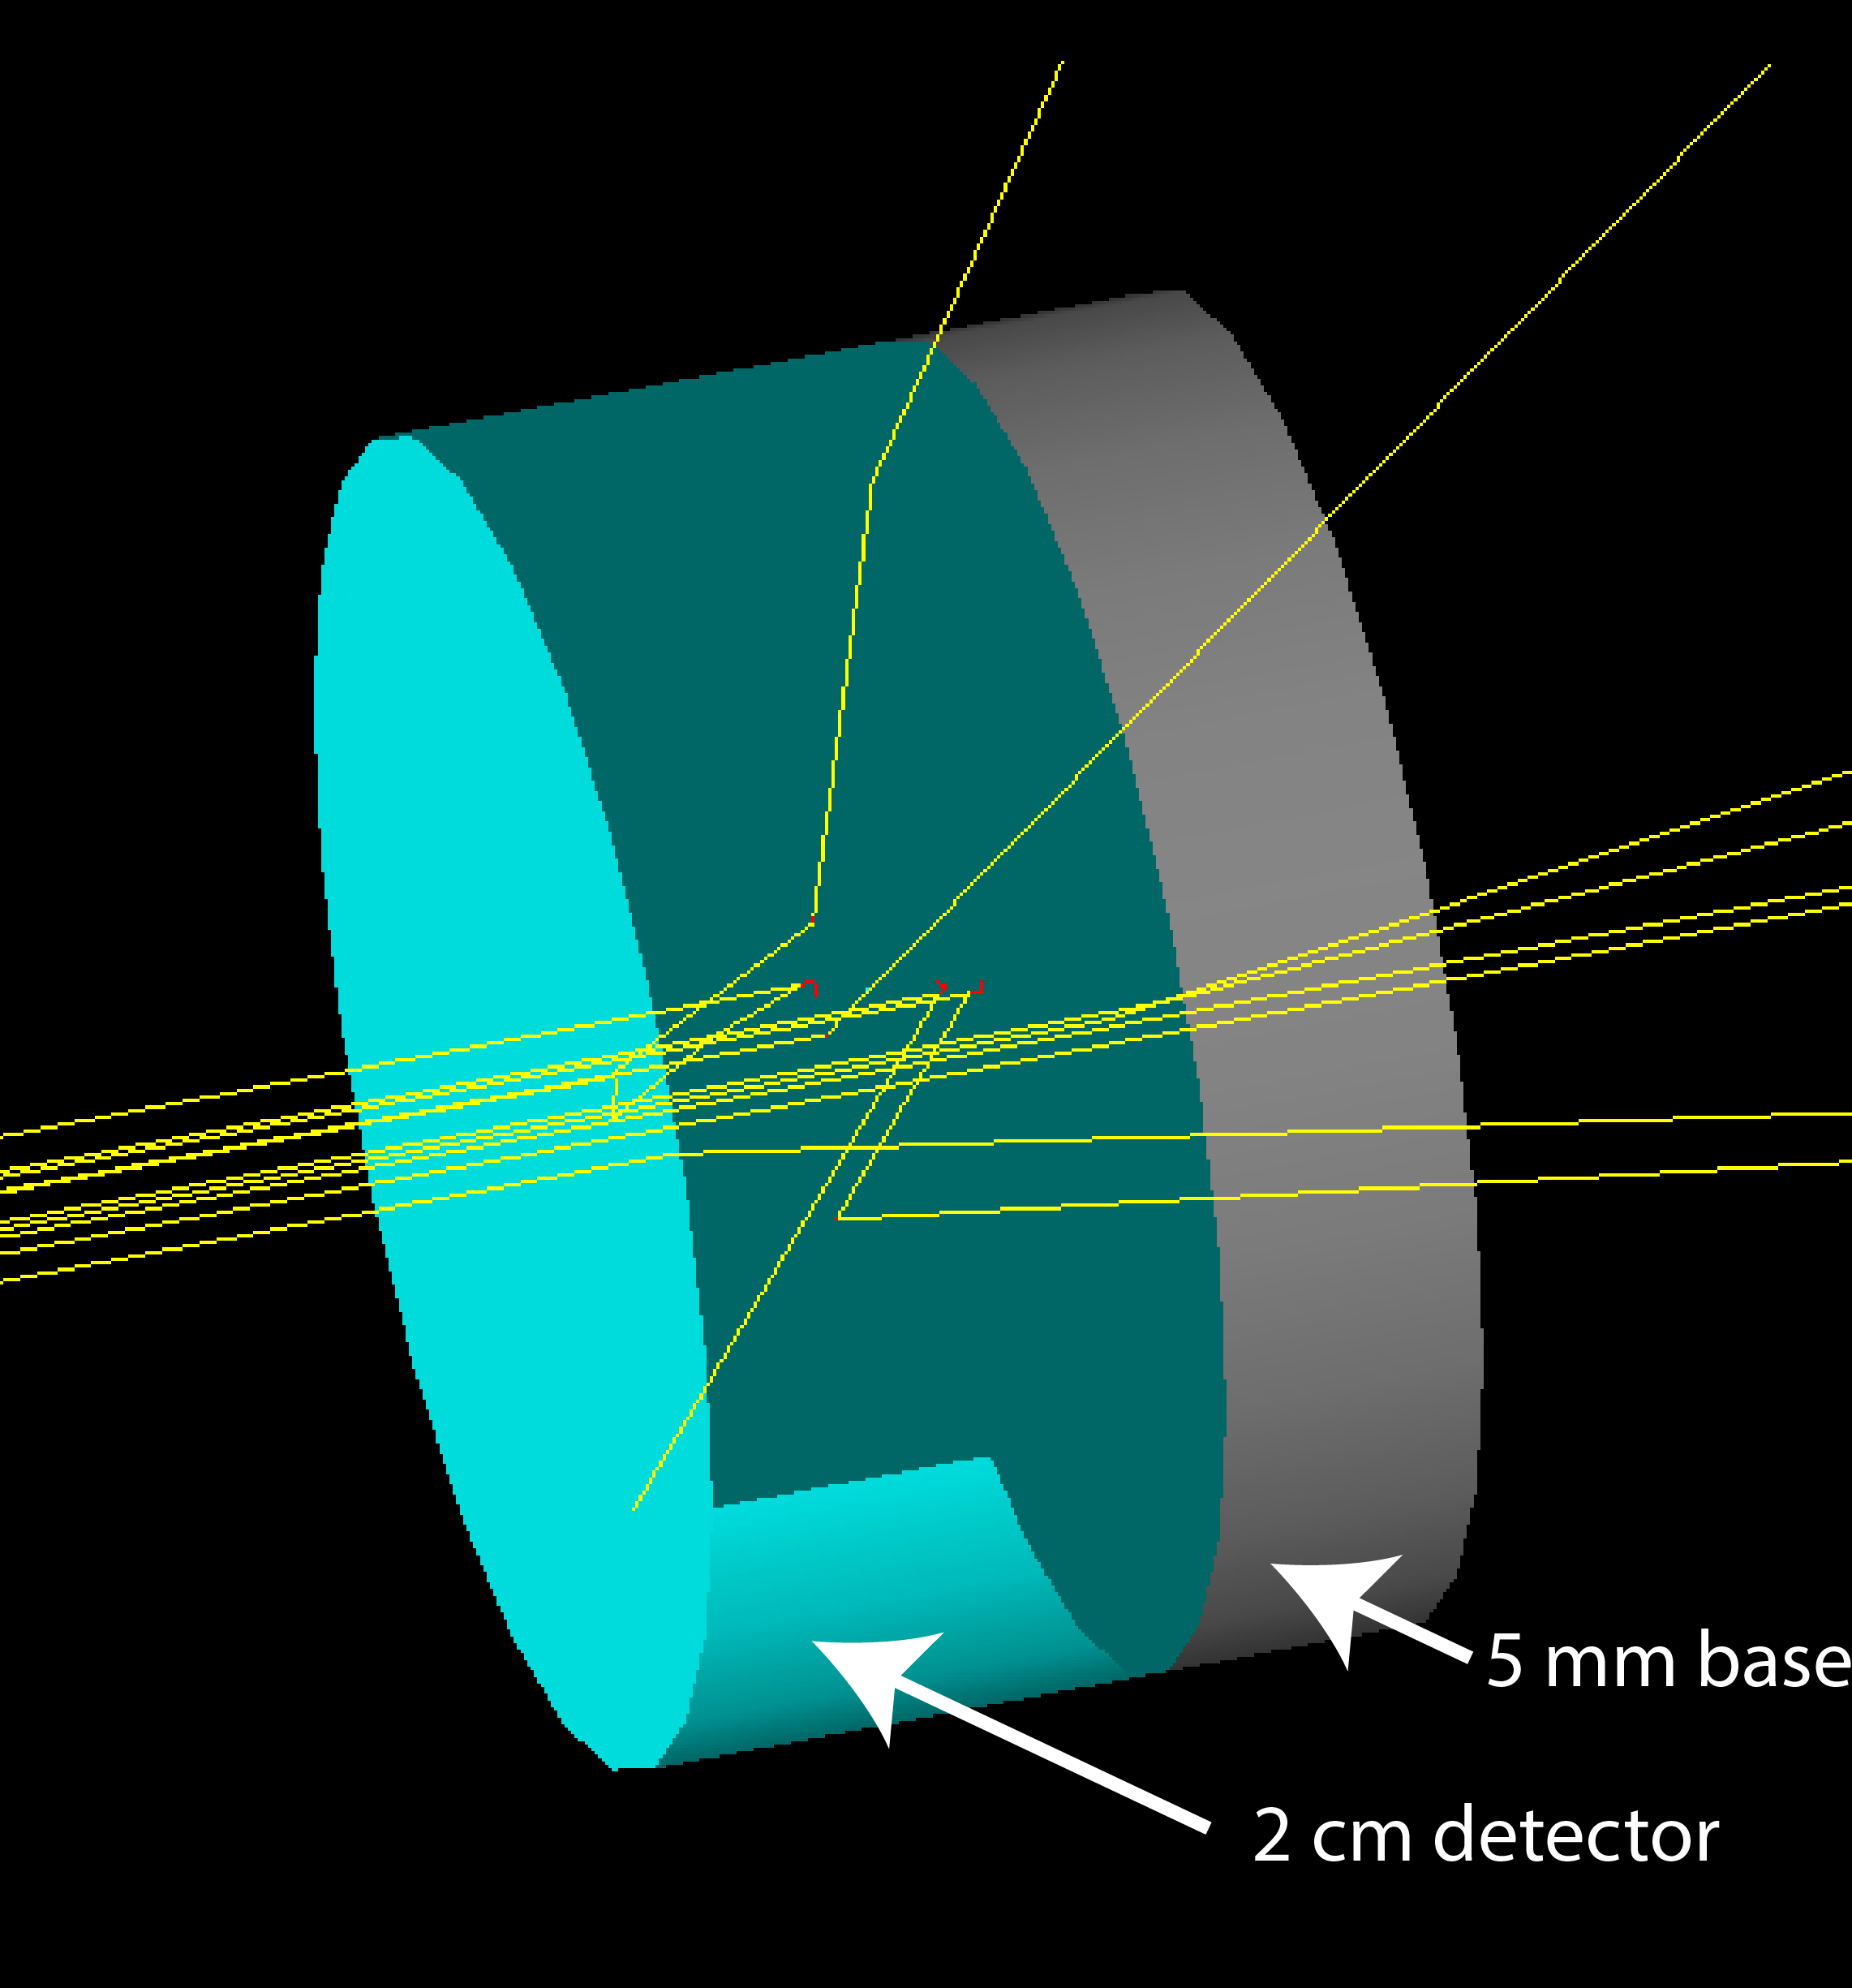
\includegraphics[width=\textwidth]{GEANT4AnnotatedGeo_EnergyDepEvent}
	\caption[GEANT4 Energy Deposition Geometry]{GEANT4 Geometry for the Simulation of Energy Deposition. What is shown are 10 photons from a \iso[60]{Co} source impingement upon a \SI{2}{\cm} thick detector.  The photon tracks are shown in yellow, while the electron tracks are shown in red.}
	\label{fig:EDepSimGeo}
\end{figure}
It is expected that the the Livermore data-driven parameterized electromagnetic physics will be necessary to calculate the ionizing energy deposition, extending the standard electro-magnetic physics down to \SI{1}{\kilo\eV}.
The neutron interactions will be simulated with a hadronic modules, using the \verb+HP+ flavored modules to use the ENDF cross sections to calculate the interaction rates.

\subsection{Simulation Validation}
The validation of this GEANT4 simulation was completed by reproducing the single collision energy loss in water as well as comparing  the spectral shapes and averages of simulated and measured spectra.
The reproduction of the single collision energy loss will ensure that the electron physics are implemented correctly, while the simulation of the polymeric film energy deposition allows the user to gain confidence that the correct tracking and binning analysis has been implemented.

\subsubsection{Single Collision Energy Loss}
The simulation was validated by reproducing the single collision energy loss for water as well as comparing spectra shapes and averages of simulated spectra to the measured spectra.
The single collision energy loss spectra for water that was simulated is shown in Figure \ref{fig:SingleCollisionELossWater}.
In general there was excellent agreement between the simulated energy spectra and a previously published spectra\cite{turner_comparative_1982}, with the simulated spectra having much better resolution than the reference did not.
It is thought that this is due to the water model in GEANT4 having better cross sections than the previously published spectra.
\begin{figure}[ht]
  \centering
  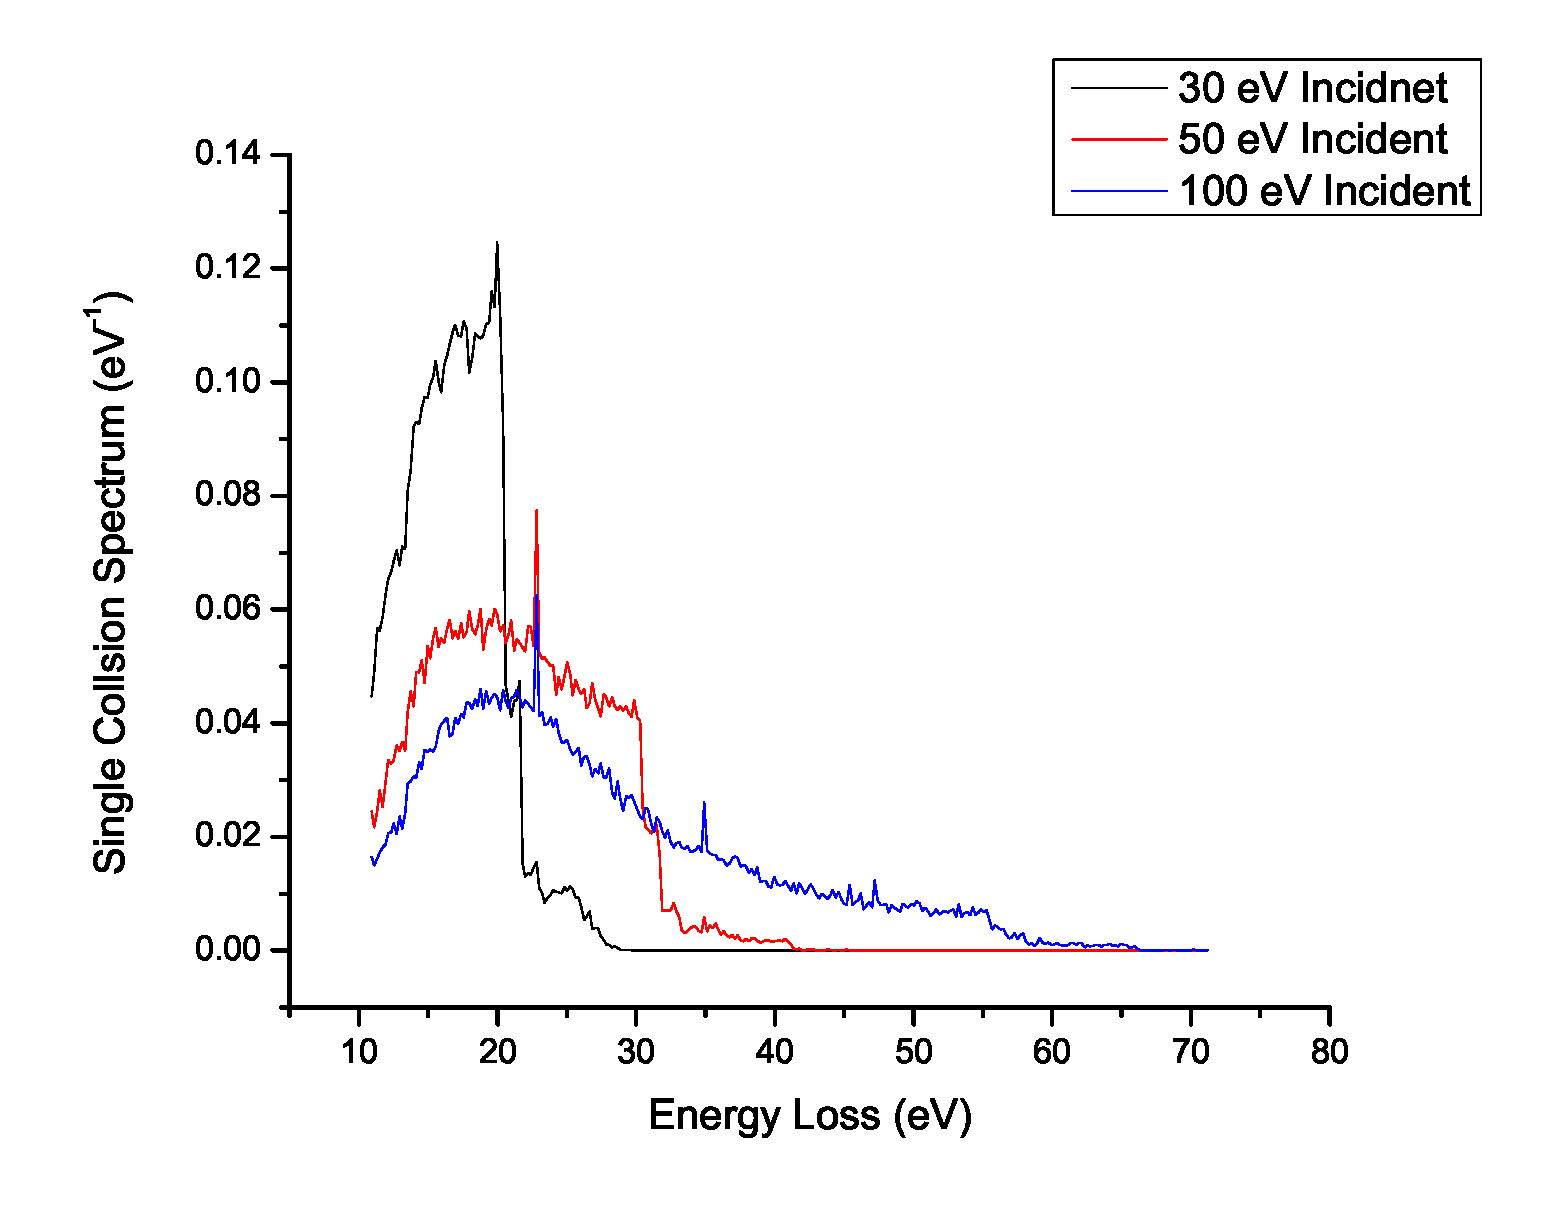
\includegraphics[width=\textwidth]{SingleCollisionEnergyLoss_300bins}
  \caption{Single Collision Energy Loss of Water. The simulated energy spectra matches that of Turner\cite{turner_comparative_1982}.}
	\label{fig:SingleCollisionELossWater}
\end{figure}

\subsubsection{Spectra Agreement}
The validity of the GEANT4 simulation is determined by comparing the spectra shapes of measured spectra to simulated energy deposition.
Figure \ref{fig:spectraComparisonGamma} shows the comparison between the simulated energy deposition per incident photon from a \iso[60]{Co} source and the measured pulse height spectra from the \iso[60]{Co} irridiator per incident photon.
The energy calibration on the upper axis of the measured spectra was completed by finding the channel number at a given intrinsic efficiency and the corresponding energy at that intrinsic efficiency.
The energy of this feature on the measured spectra was then compared to the energy on the simulated spectra, with all of the values being within 10\%.
\begin{figure*}[ht]
	\centering
	\begin{subfigure}[b]{0.45\textwidth}
    		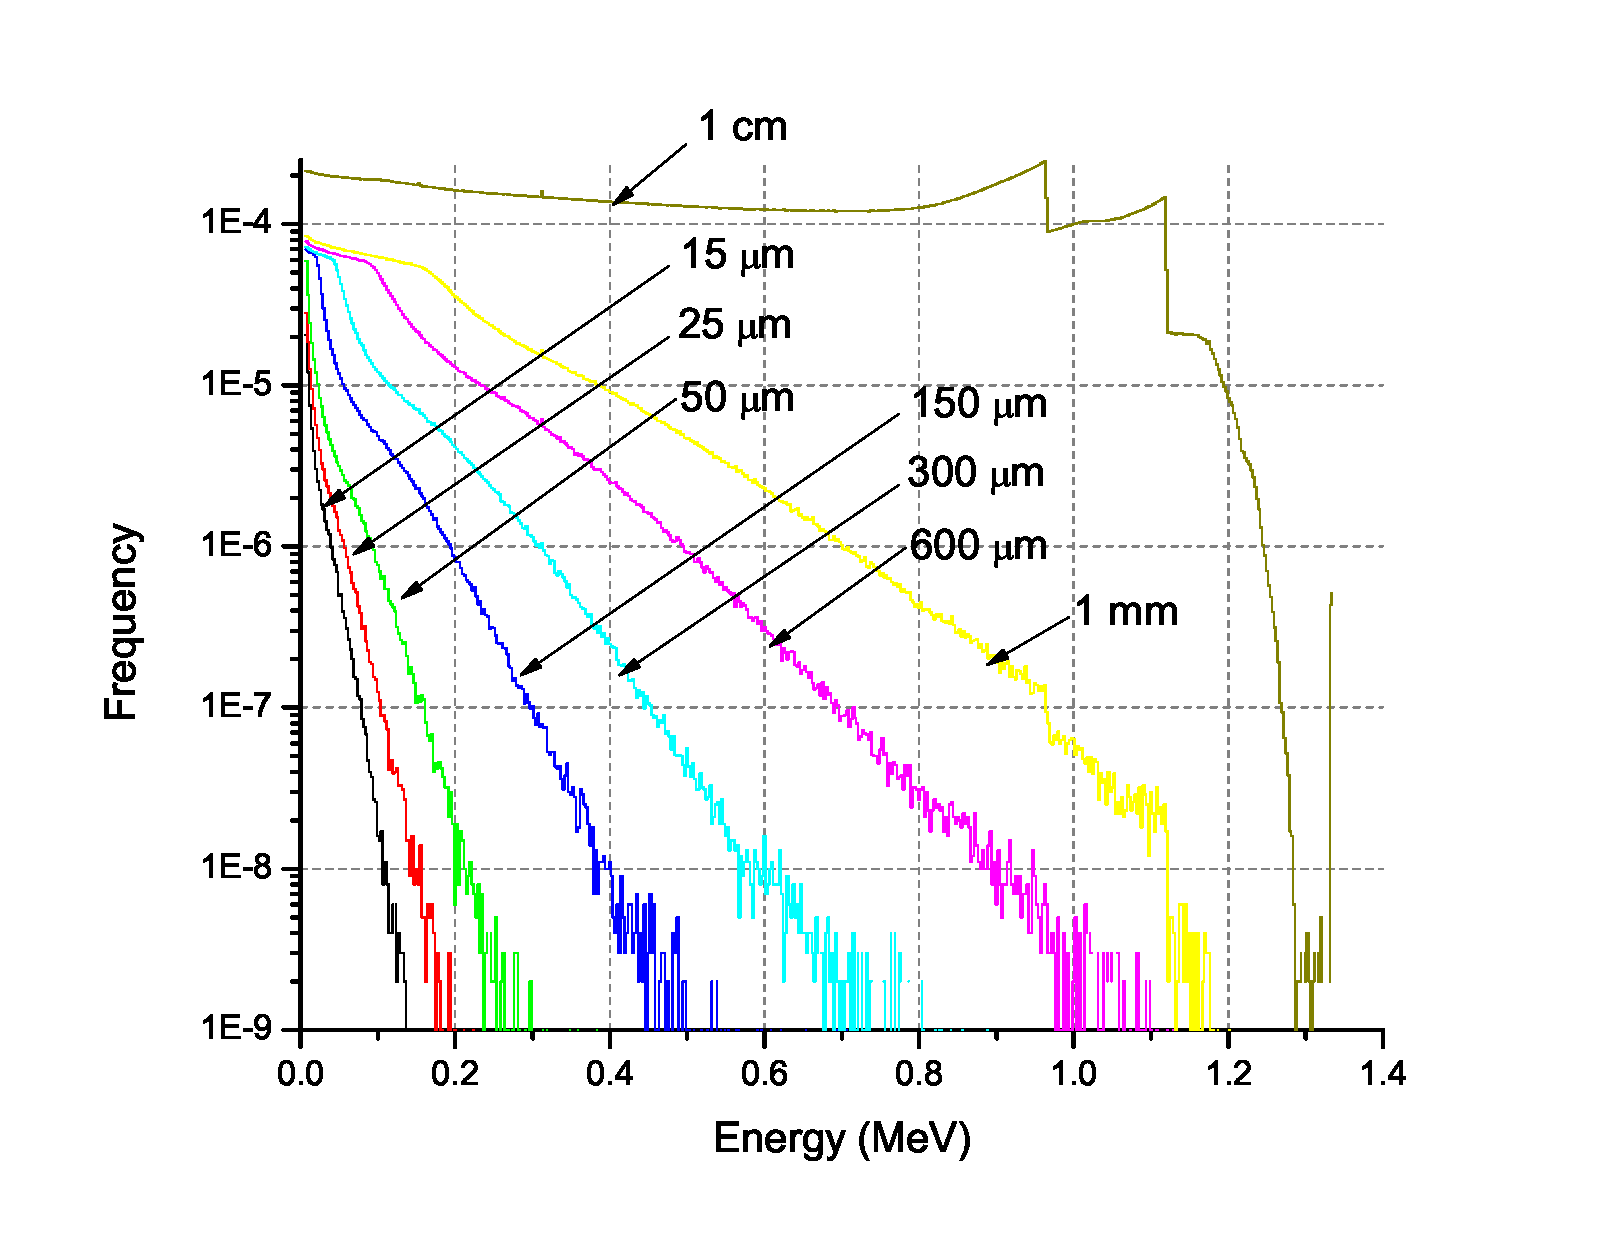
\includegraphics[width=\textwidth]{PS_EDepSim_Co60}
		\caption{GEANT4 Simulated Energy Deposition}
	\end{subfigure}%
	~
	\begin{subfigure}[b]{0.45\textwidth}
    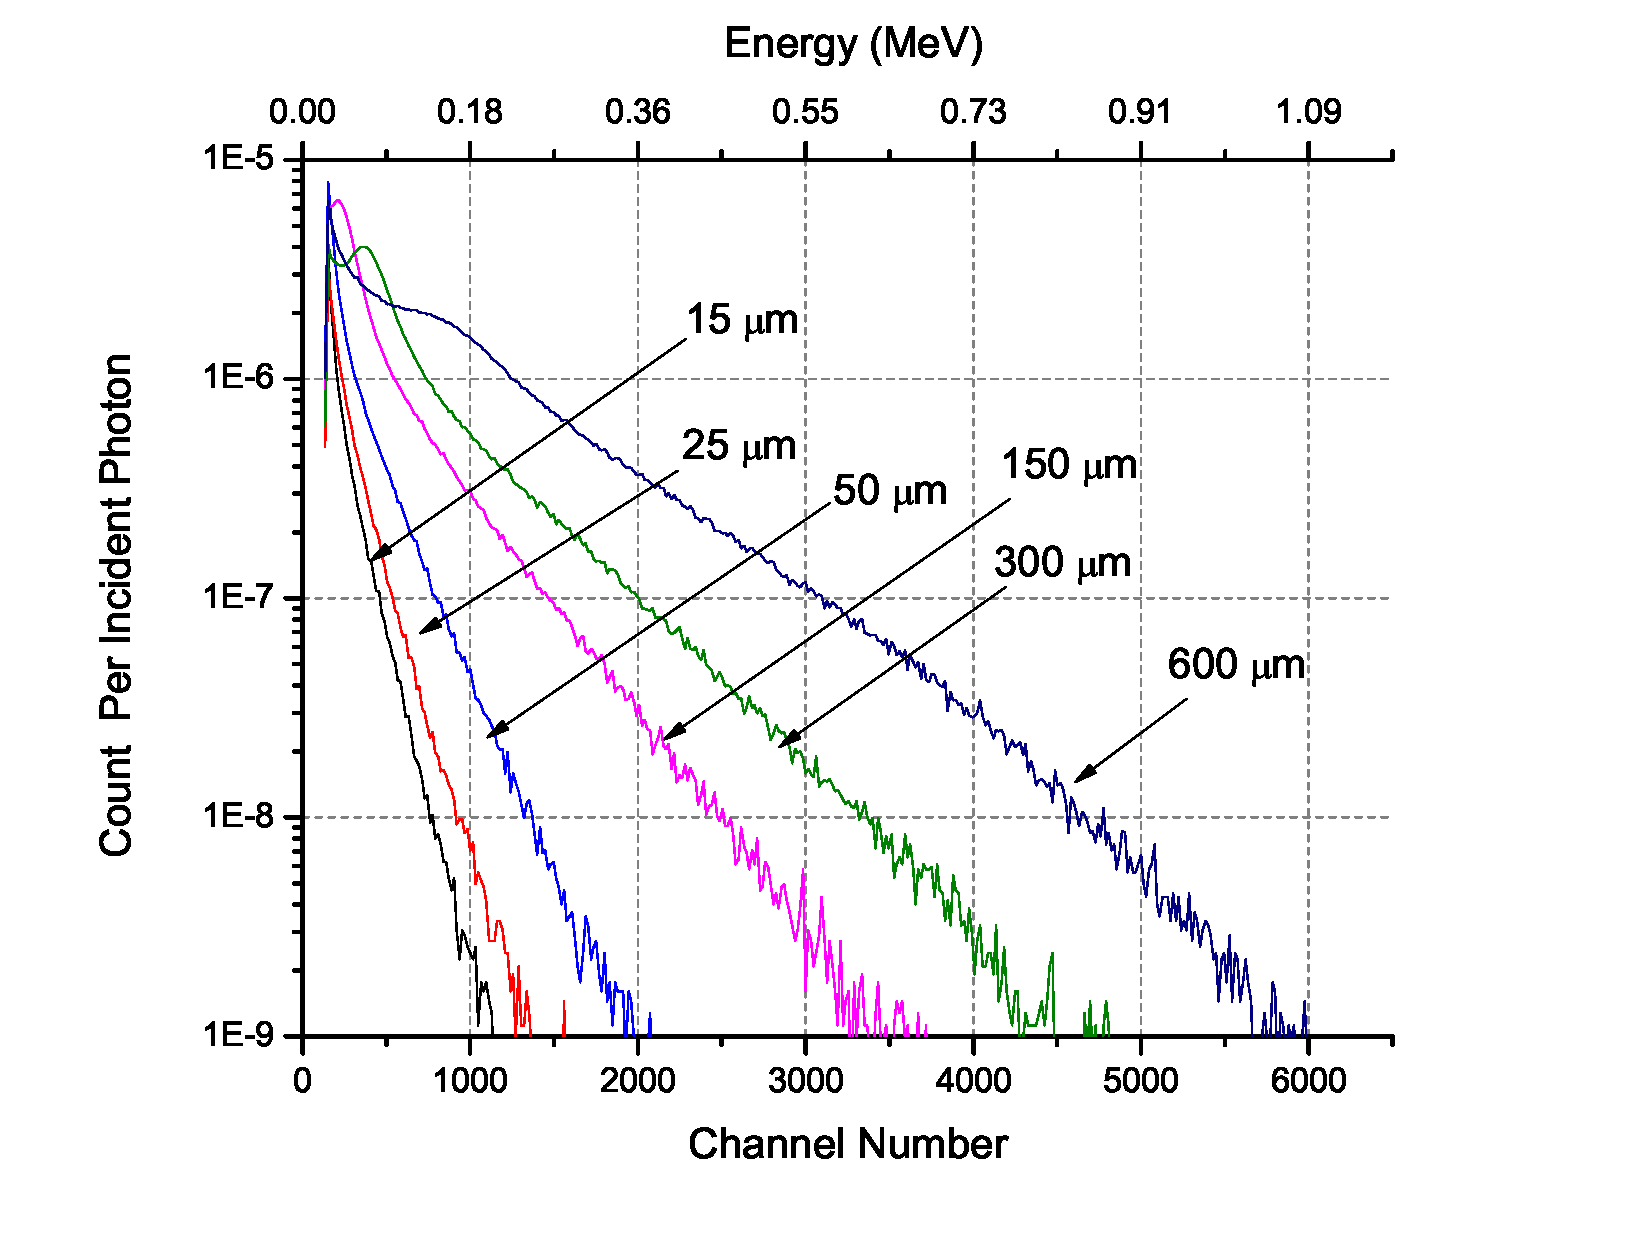
\includegraphics[width=\textwidth]{PS_GammaCR-Binned-FluxNorm_20LiF_5PPO}
		\caption{Measured Pulse Height Spectra}
	\end{subfigure}%
	\caption{Comparison of the energy deposition and binned pulse height spectra for validation. The spectra have the same shape, indicating agreement. The fabricated films greater than \SI{600}{\um} were of poor optical quality and therefore their results are not shown.}
	\label{fig:spectraComparisonGamma}
\end{figure*}
The average energy deposition and average pulse height are shown in Figure \ref{fig:EDepLightYield}. 
With the average energy deposition on the left axis and the average light yield (pulse height) on the right axis, it is possible to compare the measurement and the simulation and agreement is observed.
\begin{figure*}[ht]
	\centering
	\begin{subfigure}[b]{0.45\textwidth}
    		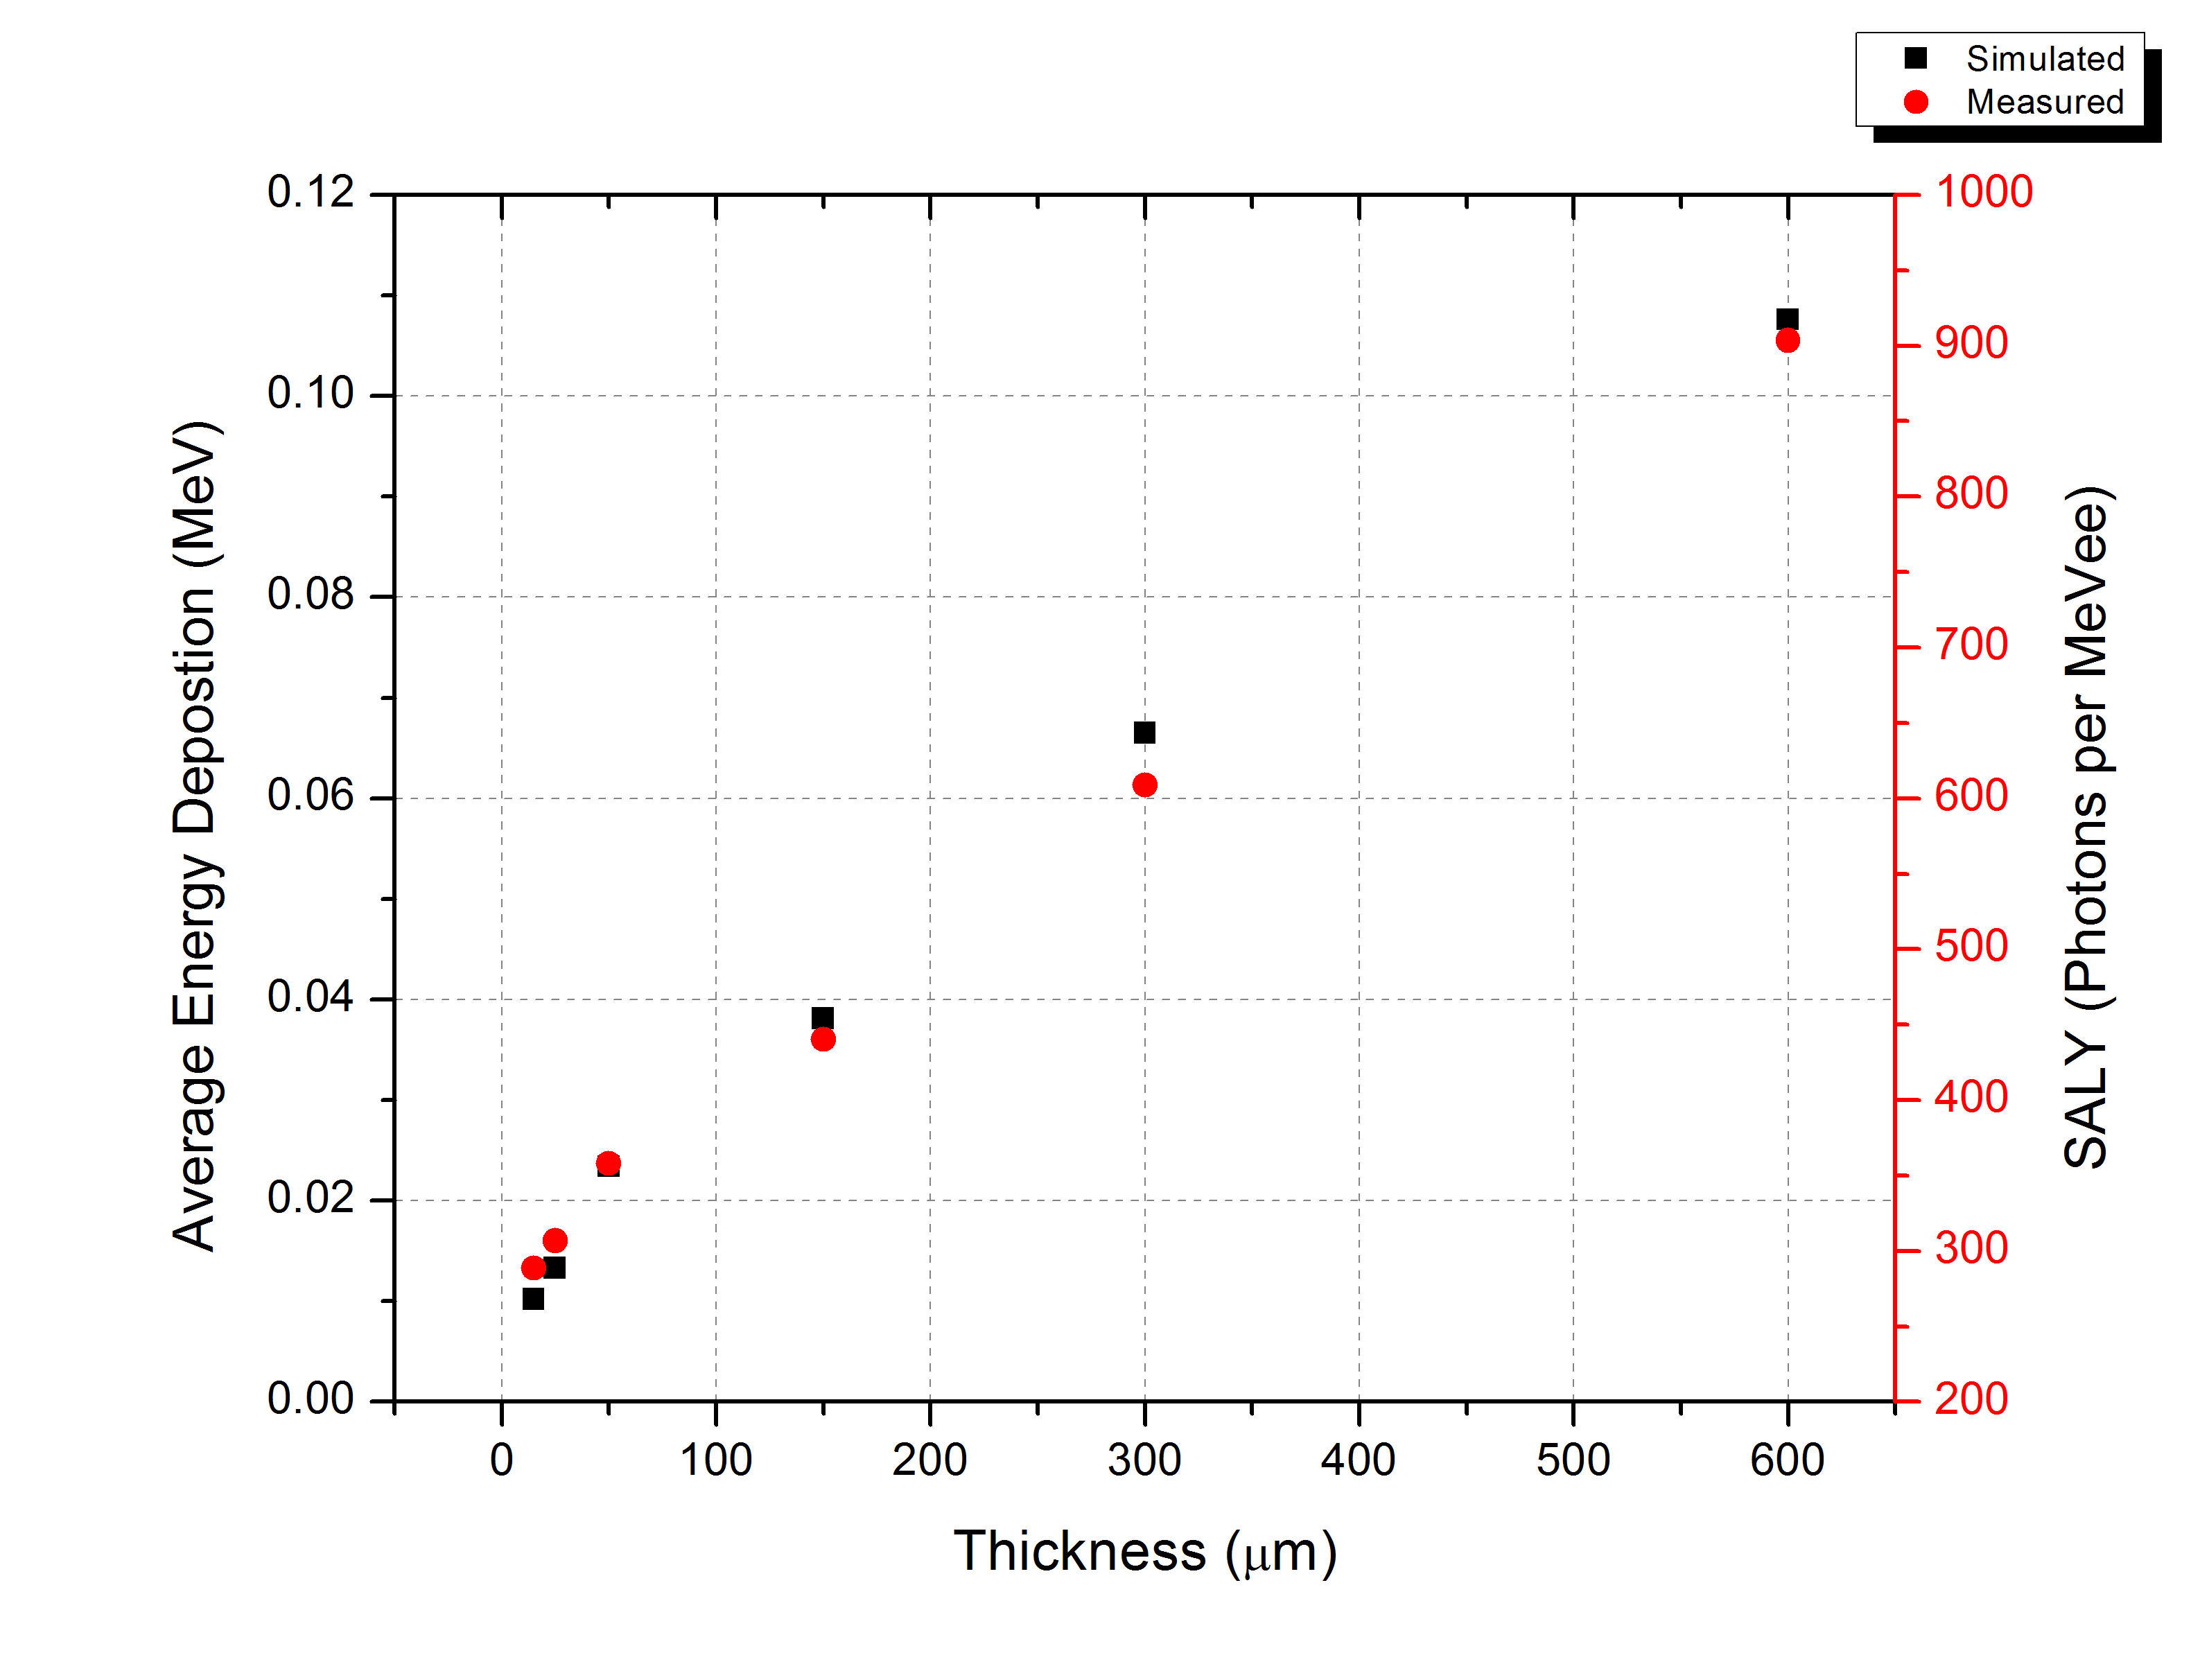
\includegraphics[width=\textwidth]{G4EDep_LightYield_Co60}
		\caption{Gamma (\iso[60]{Co})}
	\end{subfigure}%
	~
	\begin{subfigure}[b]{0.45\textwidth}
    		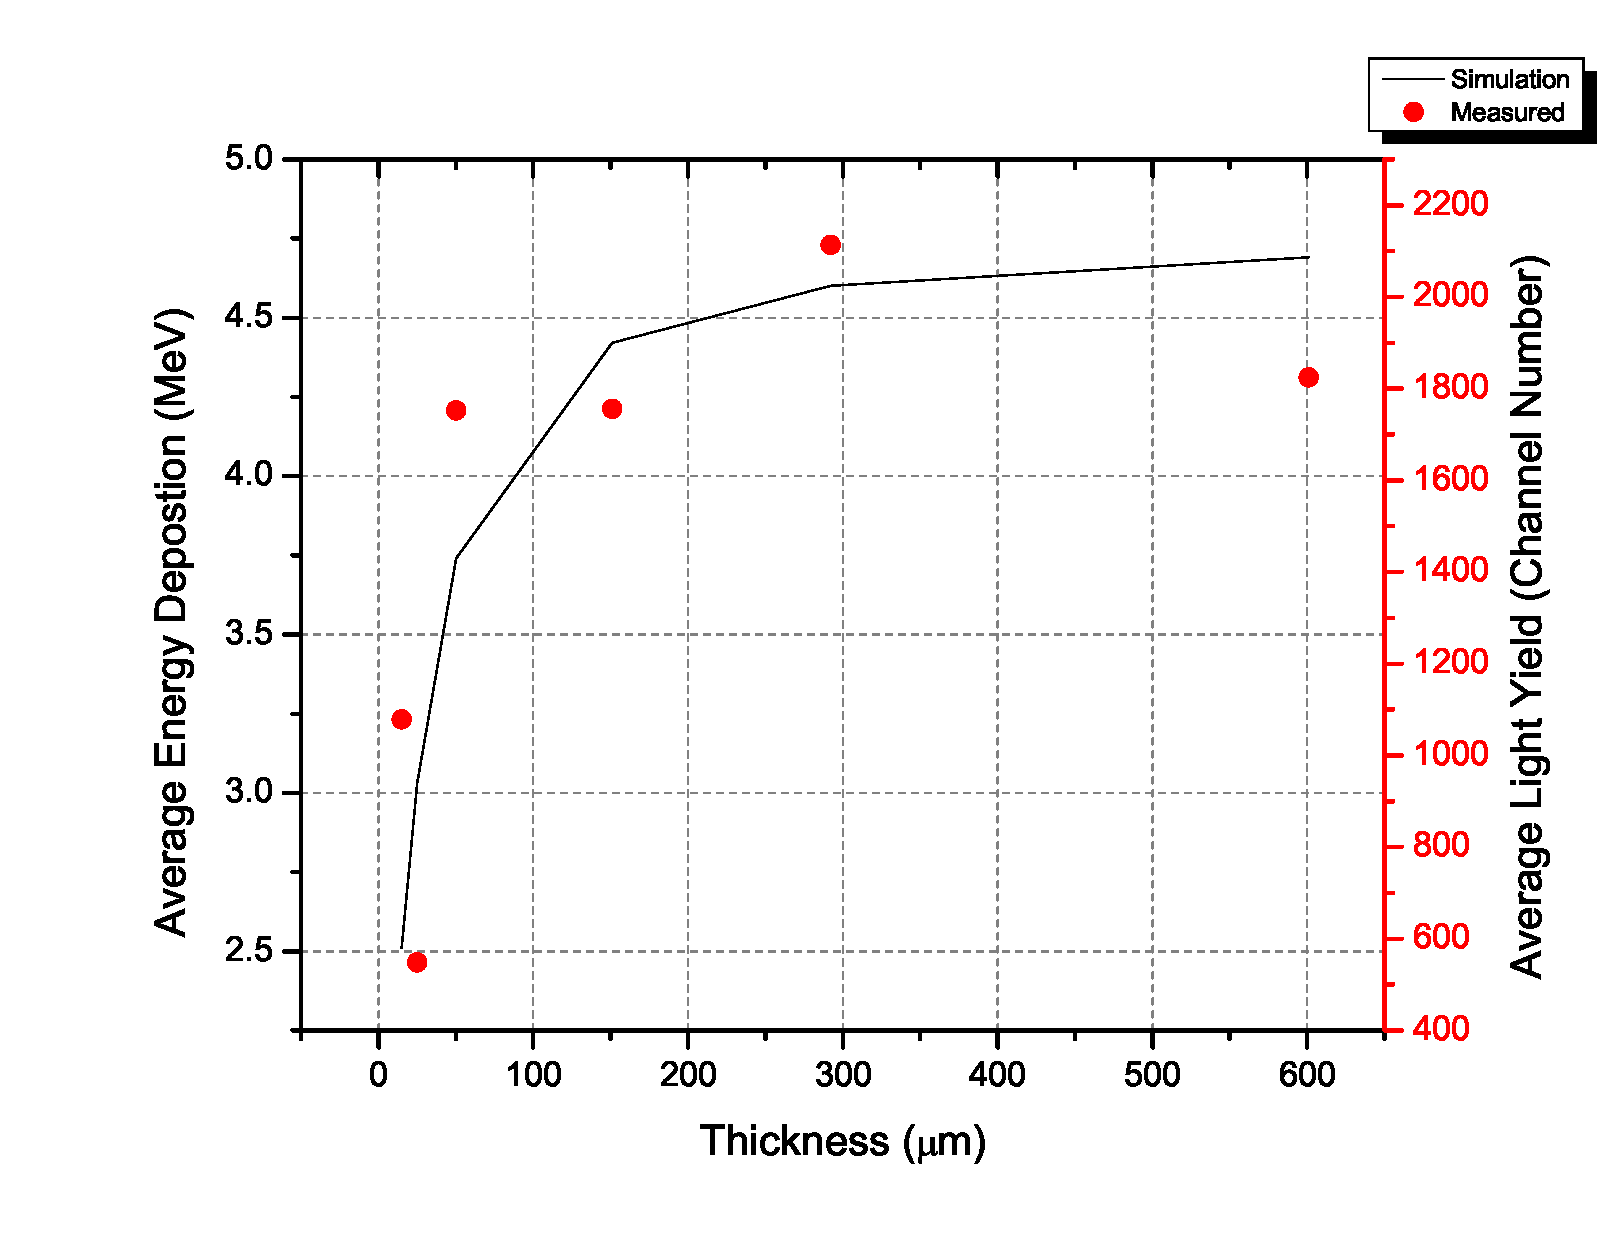
\includegraphics[width=\textwidth]{G4EDep_LightYield_Neutron}
		\caption{Neutrons}
	\end{subfigure}%
	\caption{Average Energy Deposition and Measured Light Yield. The solid lines are calculated values and the red dots are measurements.}
	\label{fig:EDepLightYield}
\end{figure*}


%%%%%%%%%%%%%%%%%%%%%%%%%%%%%%%%%%%%%%%%%%%%%%%%%%%%%%%%%%%%%%%%%%%%%%%%%%%
%                                                                         %
%                     RESULTS and ANALYSIS                                %
%                                                                         %
%%%%%%%%%%%%%%%%%%%%%%%%%%%%%%%%%%%%%%%%%%%%%%%%%%%%%%%%%%%%%%%%%%%%%%%%%%%
\section{Results}
\label{sec:Results}

The average energy deposited by a neutron and gamma reaction was investigated for different film thickness to determine if an optimal thickness does exits in a geometry similar to \autoref{fig:EDepSimGeo}.
\autoref{fig:SimEDep} shows that the energy deposition of the gamma quickly falls off as the films get thinner, while it isn't util the neutron films become on the order of the range of the triton that the energy deposition is impacted.
\autoref{fig:EDepPosSim} examines the impact of where the interaction took place in the film on the energy deposition.
The geometry for this simulation is once again \autoref{fig:EDepSimGeo}, where the beam spot is \SI{3}{\mm} and the area of the detector face is \SI{10}{\cm}. 
The interaction position is then defined to be distance to the first interaction of the beam in the material along the direction of the beam.
It is obseved that for neutrons events that take place within the center of the films tend to deposit a large majority of their energy in the film, while events that occur on the edge of the film have partial energy depositions in accordance with the ranges of the charged particles.
A compton spectra is obseved in the photon energy deposition. 
A secondary effect in having a backing material is also observed for photons in which there is a hightened energy deposition for interactions that occur in the film but near the boundary and electrons are back scattered into the detector material.
\begin{figure}
  \centering
  \incluegraphics[width=0.6\textwidth]{SimulatedEnergyDeposition}
  \caption[Simulated Energy Deposition and Film Thickness]{Simulated energy deposition and film thickness.  As the films get much thinner it is very unlikely for gamma events to deposition all of their energy, while above \SI{50}{\um} there is very little impact on the energy deposited by neturons.}
  \label{fig:SimEDep}
\end{figure}

\begin{figure*}[ht]
	\centering
	\begin{subfigure}[b]{0.45\textwidth}
    		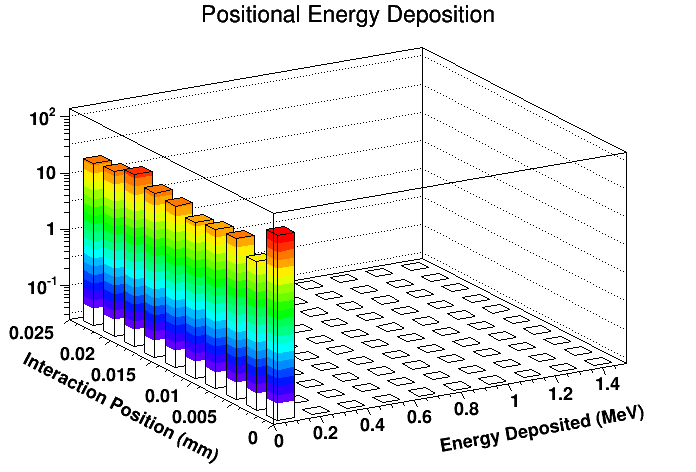
\includegraphics[width=\textwidth]{posEDepCo600.025}
		\caption{ \SI{25}{\um} Gamma (\iso[60]{Co})}
	\end{subfigure}%
	~
	\begin{subfigure}[b]{0.45\textwidth}
    		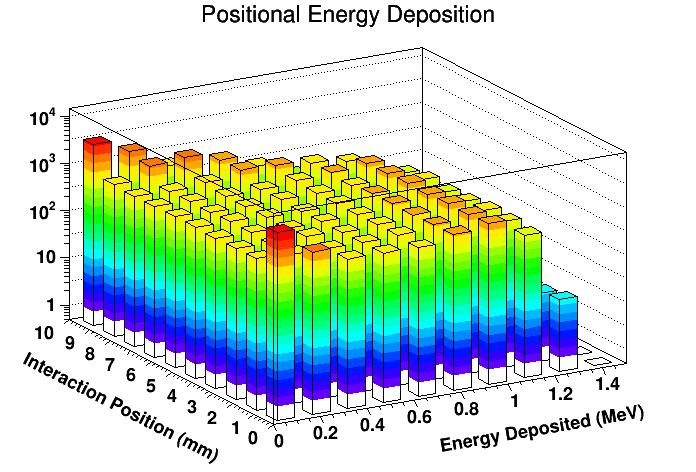
\includegraphics[width=\textwidth]{posEDepCo6010.0}
		  \caption{ \SI{1}{\cm} Gamma (\iso[60]{Co})}
	\end{subfigure}%
	
  \begin{subfigure}[b]{0.45\textwidth}
    		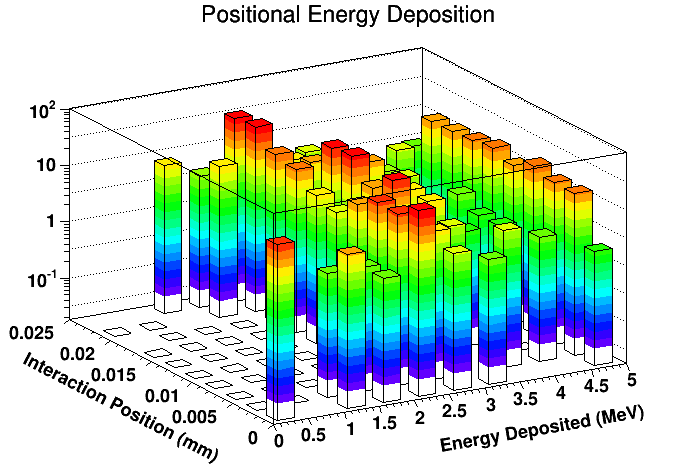
\includegraphics[width=\textwidth]{posEDepneutron0.025}
		\caption{ \SI{25}{\um} Neutron}
	\end{subfigure}%
	~
	\begin{subfigure}[b]{0.45\textwidth}
    		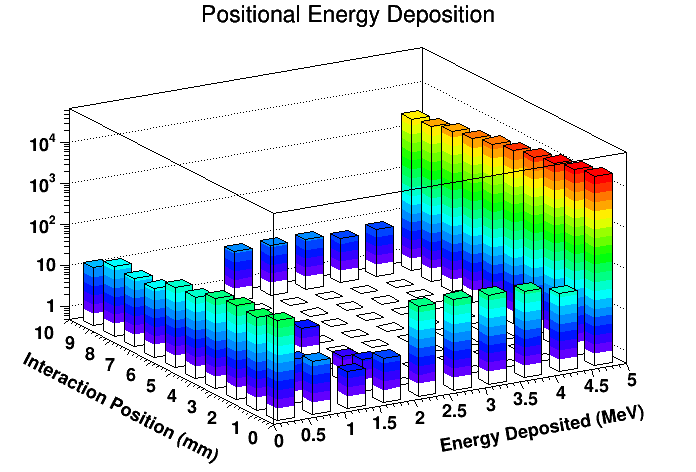
\includegraphics[width=\textwidth]{posEDepneutron10.0}
		  \caption{ \SI{1}{\cm} Neutron}
	\end{subfigure}%
	\caption[Simulated Energy Deposition and Position]{Simulated average energy depositions and the position of the first interactions. The beam is considered to be incident on position 0, and thus interactions that occur on the front of the film have a much higher probability deposting all of their energy. Events that occur on the edge of the film much less likely to deposit all of their available energy.}
	\label{fig:EDepPosSim}
\end{figure*}

The energy deposition and light yield were also investigated by simulations in the GEANT4 enviroment for polystyrene based films (light output 1,000 photons per MeV).
These simulations (summerized in \autoref{fig:EDepLightYield}) show that as expected the light output was linear with the energy deposition.
\begin{figure*}[ht]
	\centering
	\begin{subfigure}[b]{0.45\textwidth}
    		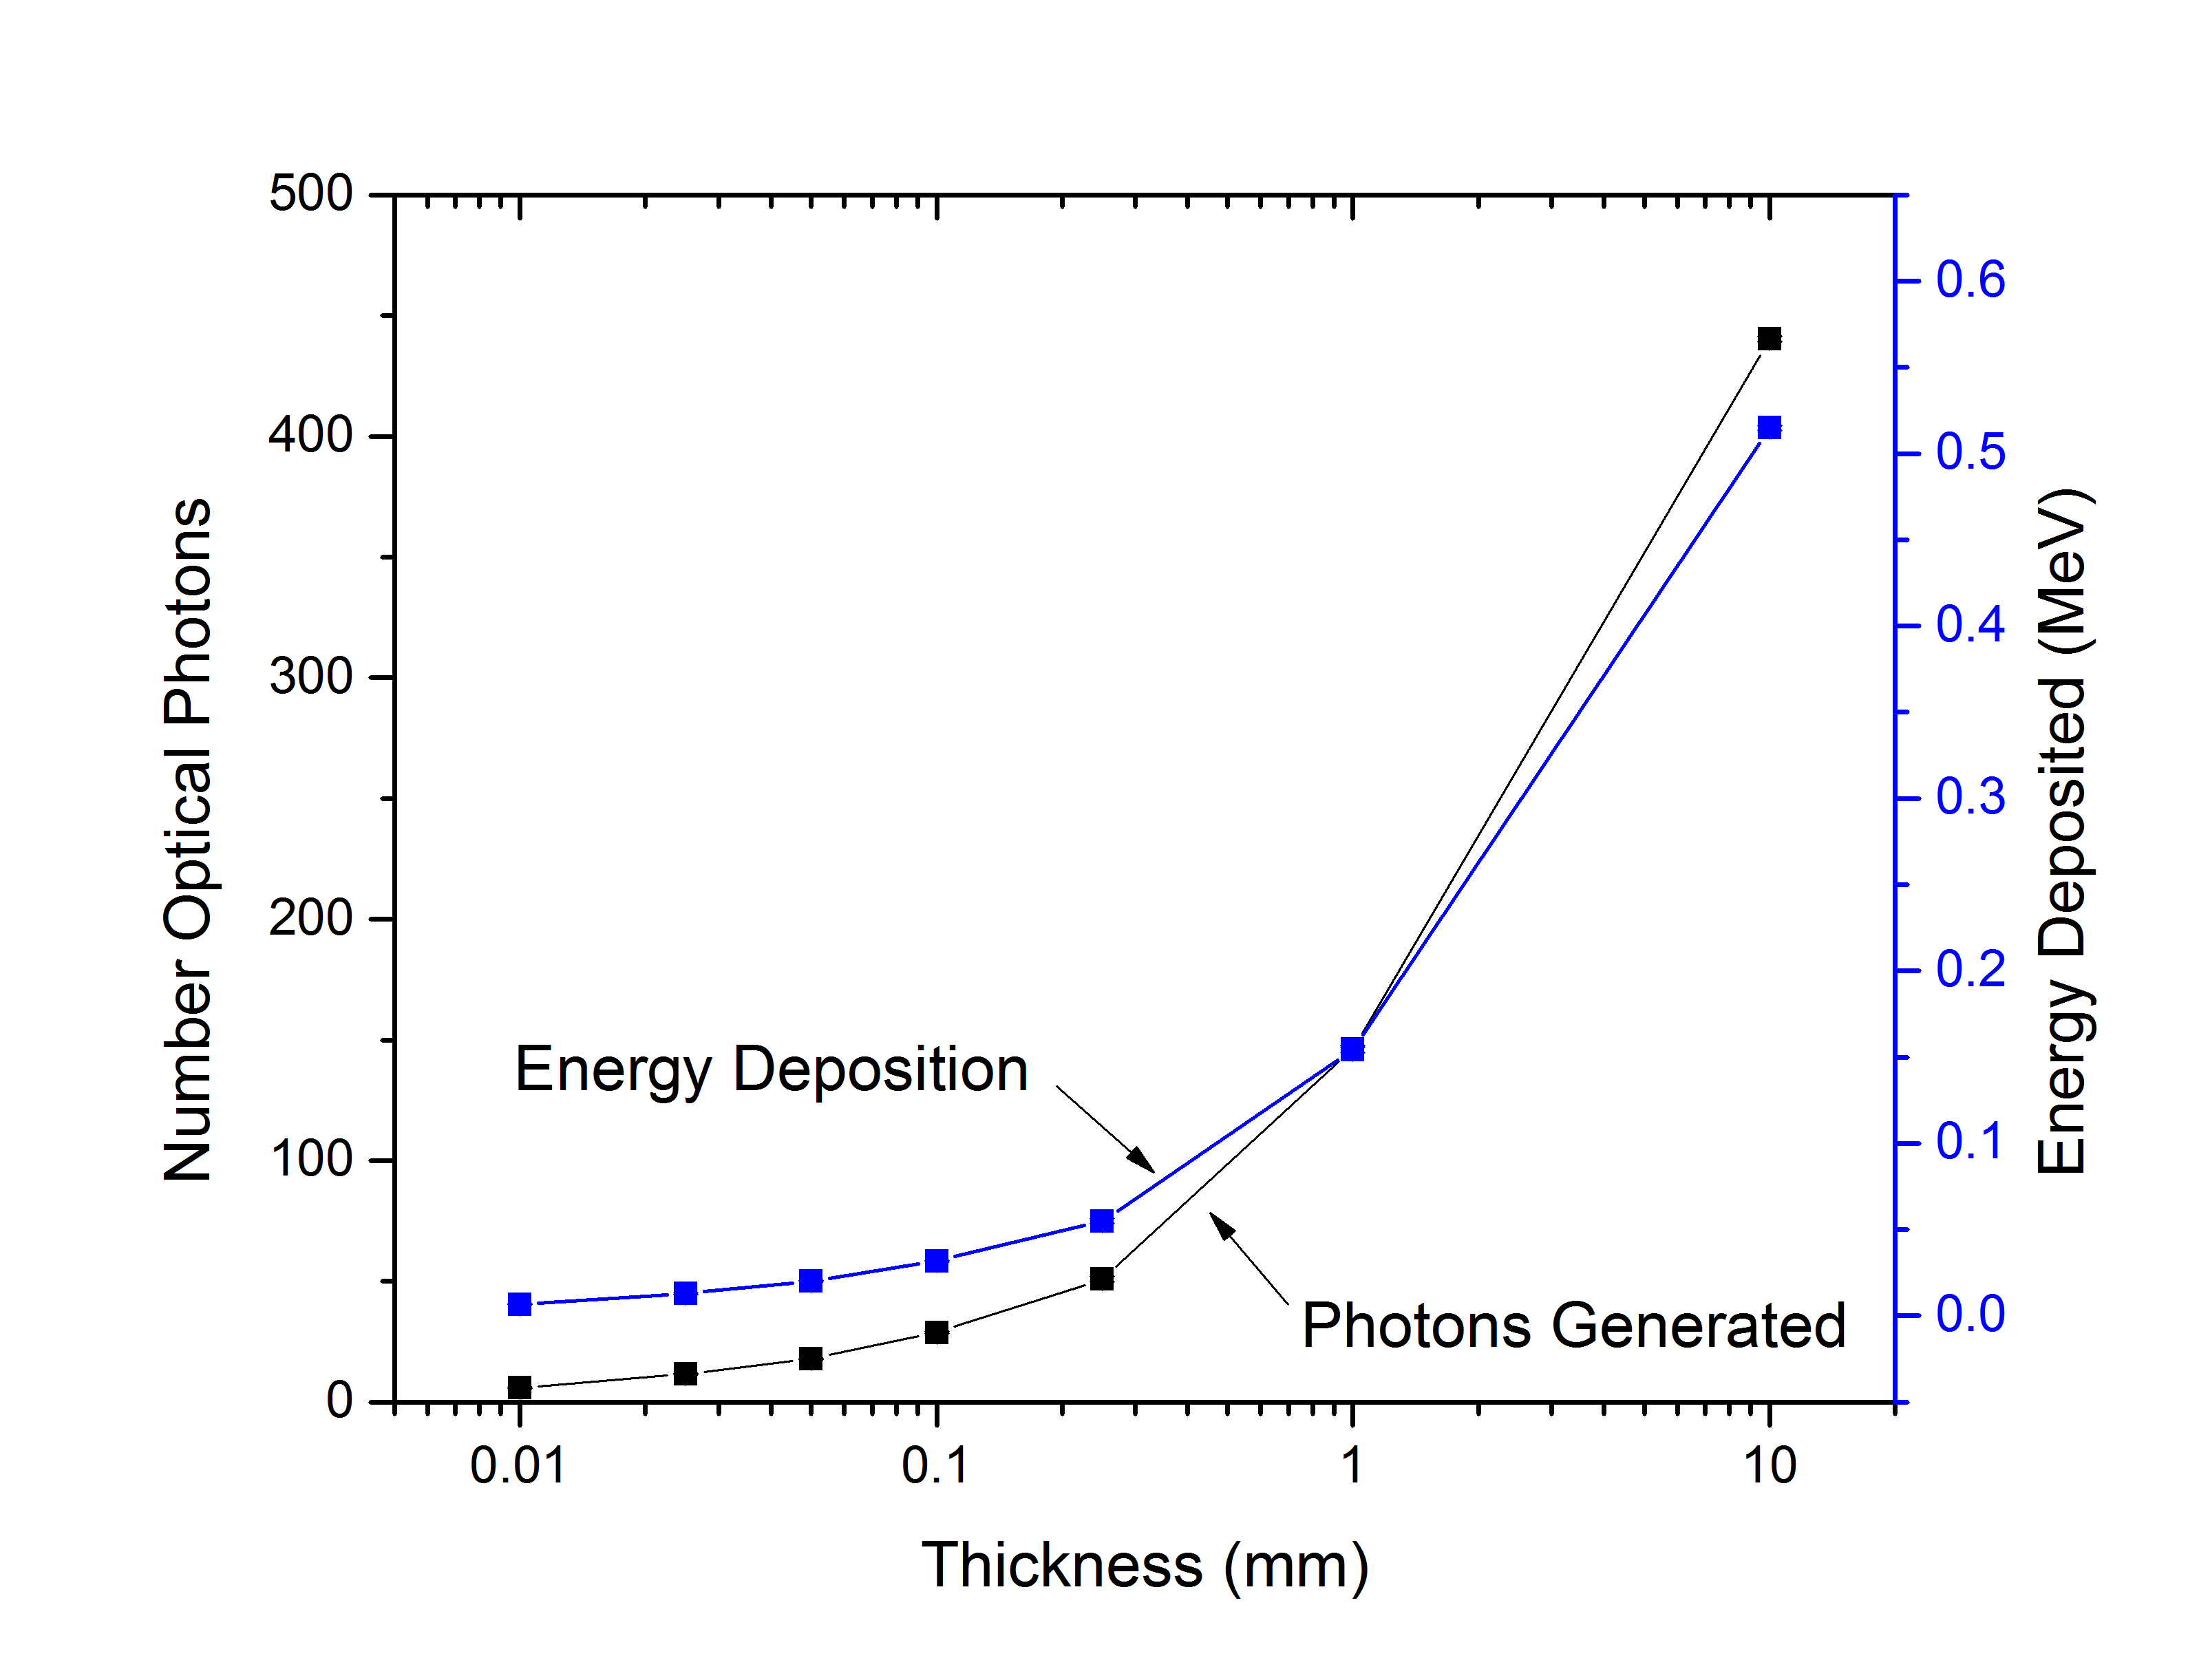
\includegraphics[width=\textwidth]{EDepLightYield_Gamma}
		\caption{ Gamma (\iso[60]{Co}}
	\end{subfigure}%
	~
	\begin{subfigure}[b]{0.45\textwidth}
    		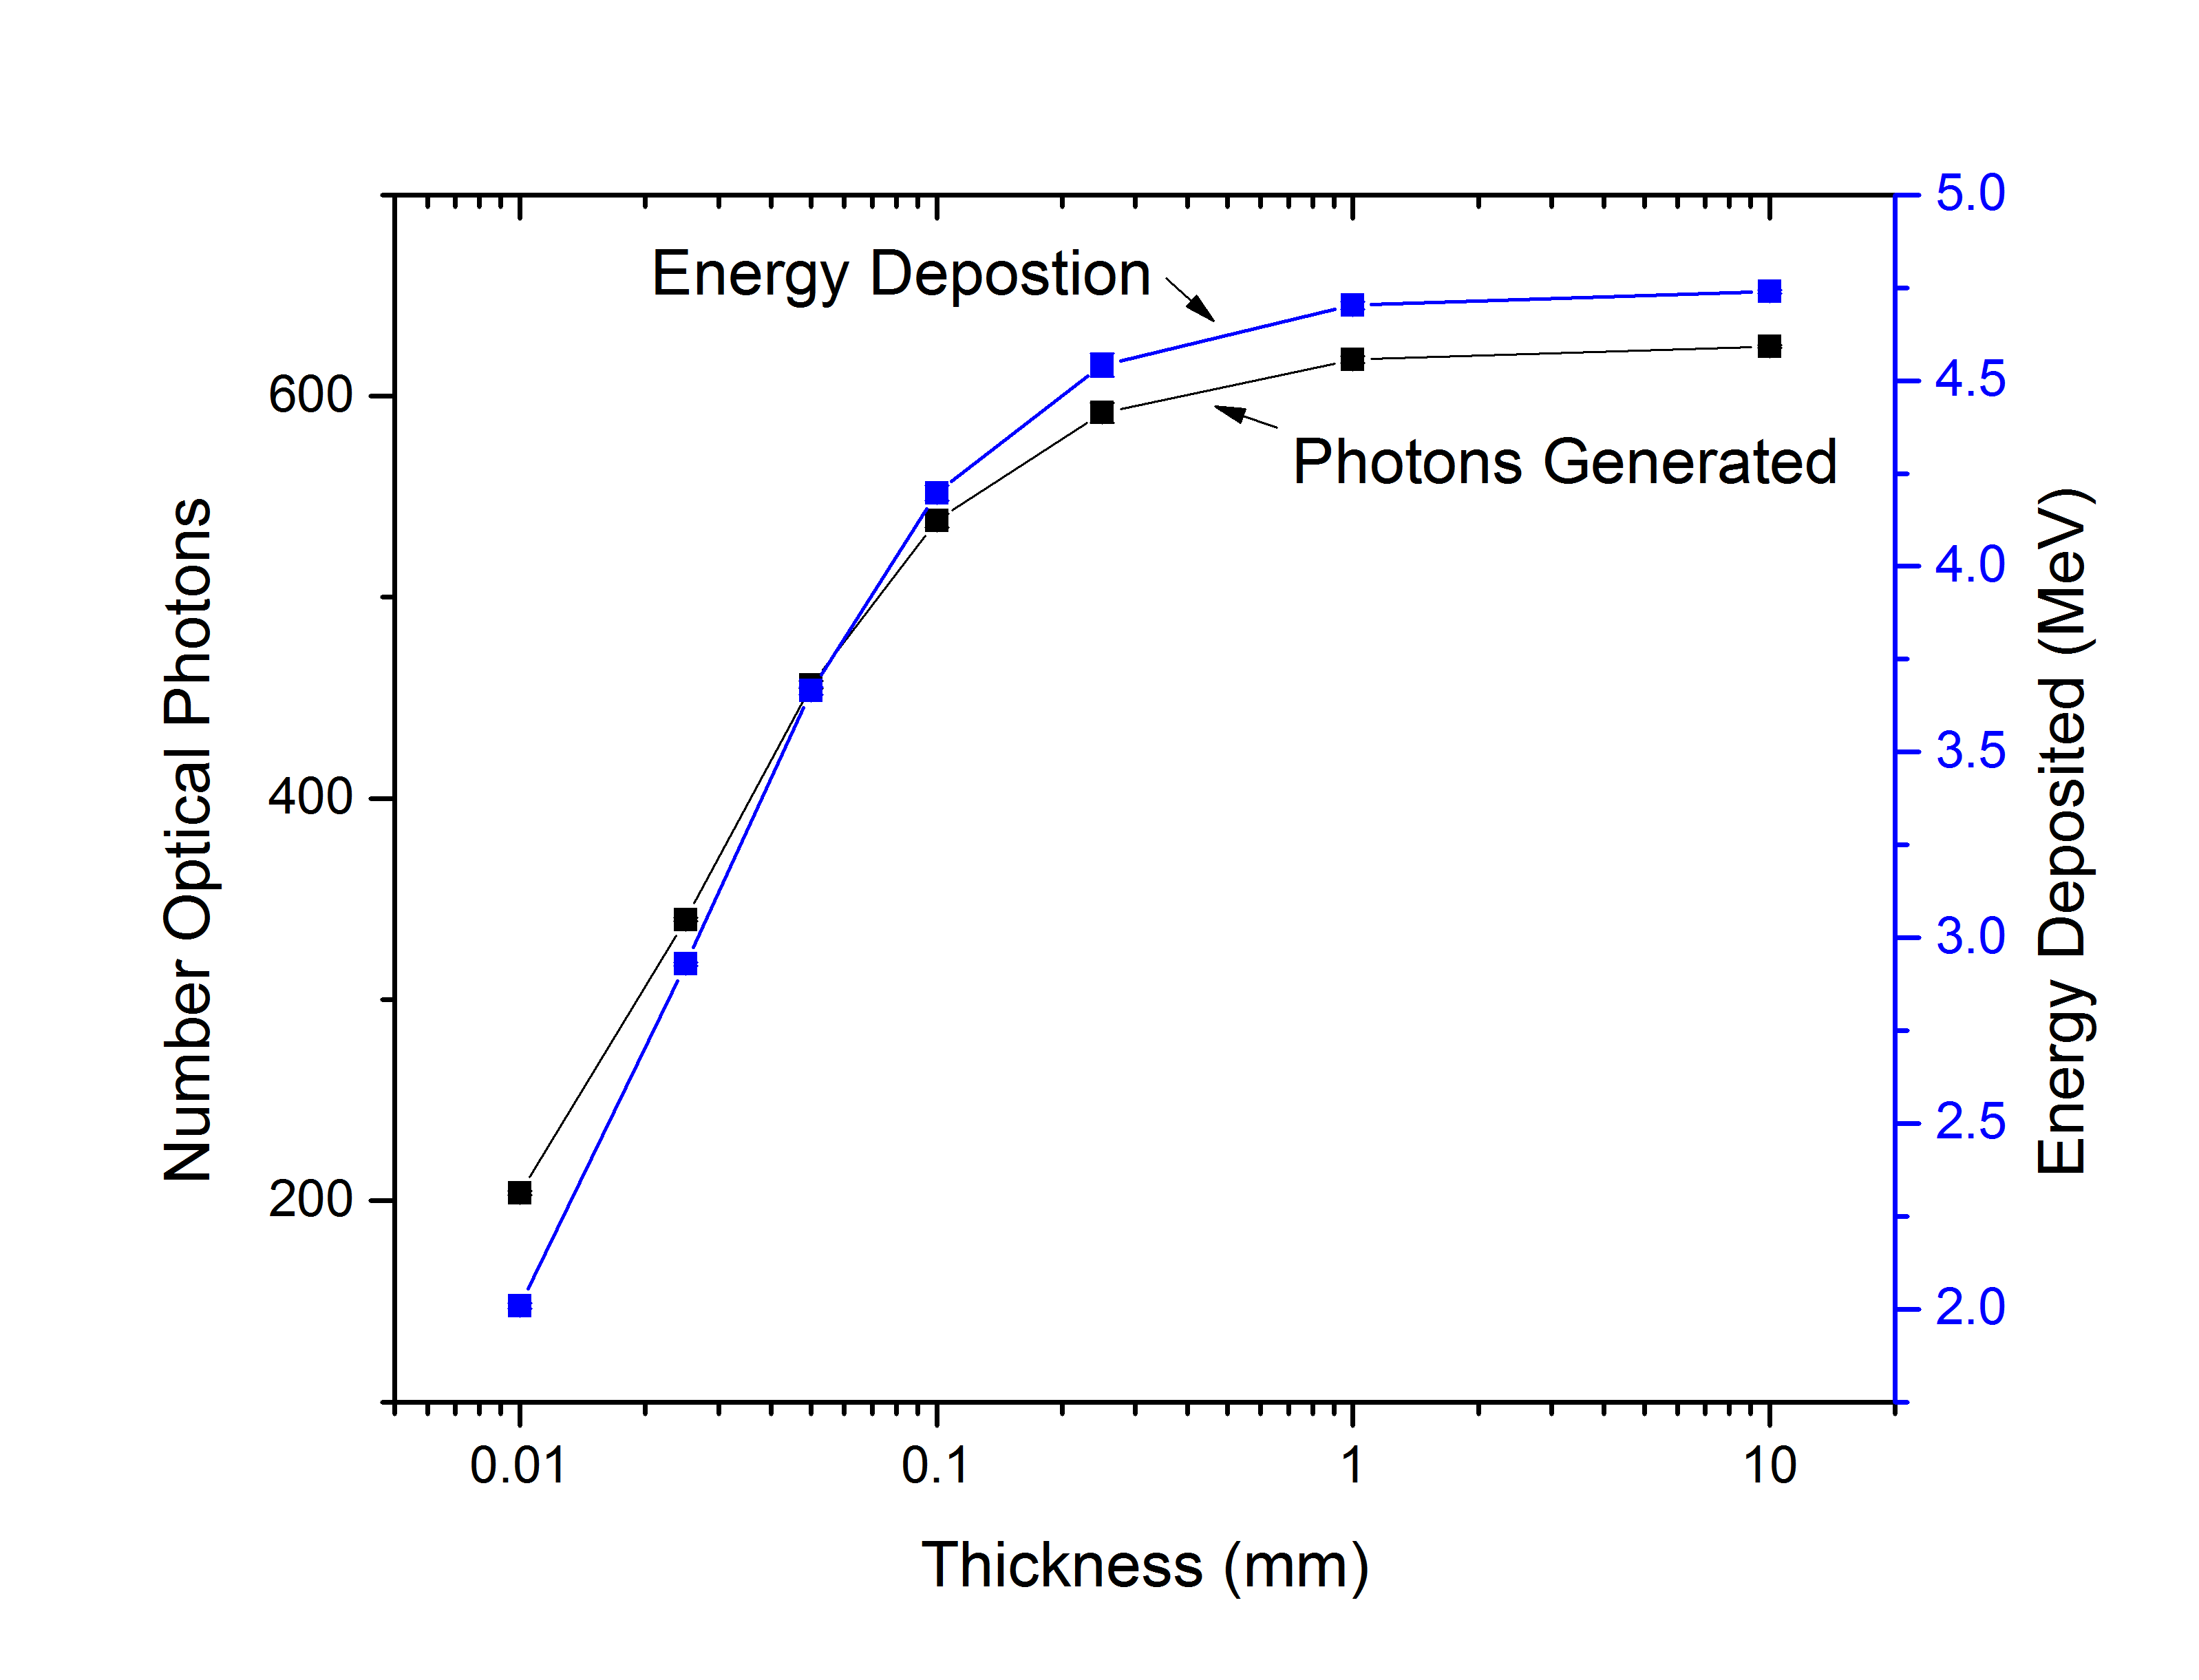
\includegraphics[width=\textwidth]{EDepLightYield_Neutron}
		  \caption{ Neutron}
	\end{subfigure}%
  \caption[Energy Depostion and Light Yield]{Simulated energy deposition and light yield.  The light yield is fairly linear with the energy deposition, thus, the energy deposition is an adaquate indicator of the expected light yield.}
  \label{fig:EDepLightYield}
\end{figure*}
However, it is instructive to look at the distrubtions of how many photons were created per event.
As the films get thicker and more of the triton energy is capture the resonse of the triton starts to dominate the alpha (\autoref{fig:NeutronPhotonsGenSim}).
For photons, shown in \autoref{fig:GammaPhotonsGenSim},
\begin{figure}
  \centering
  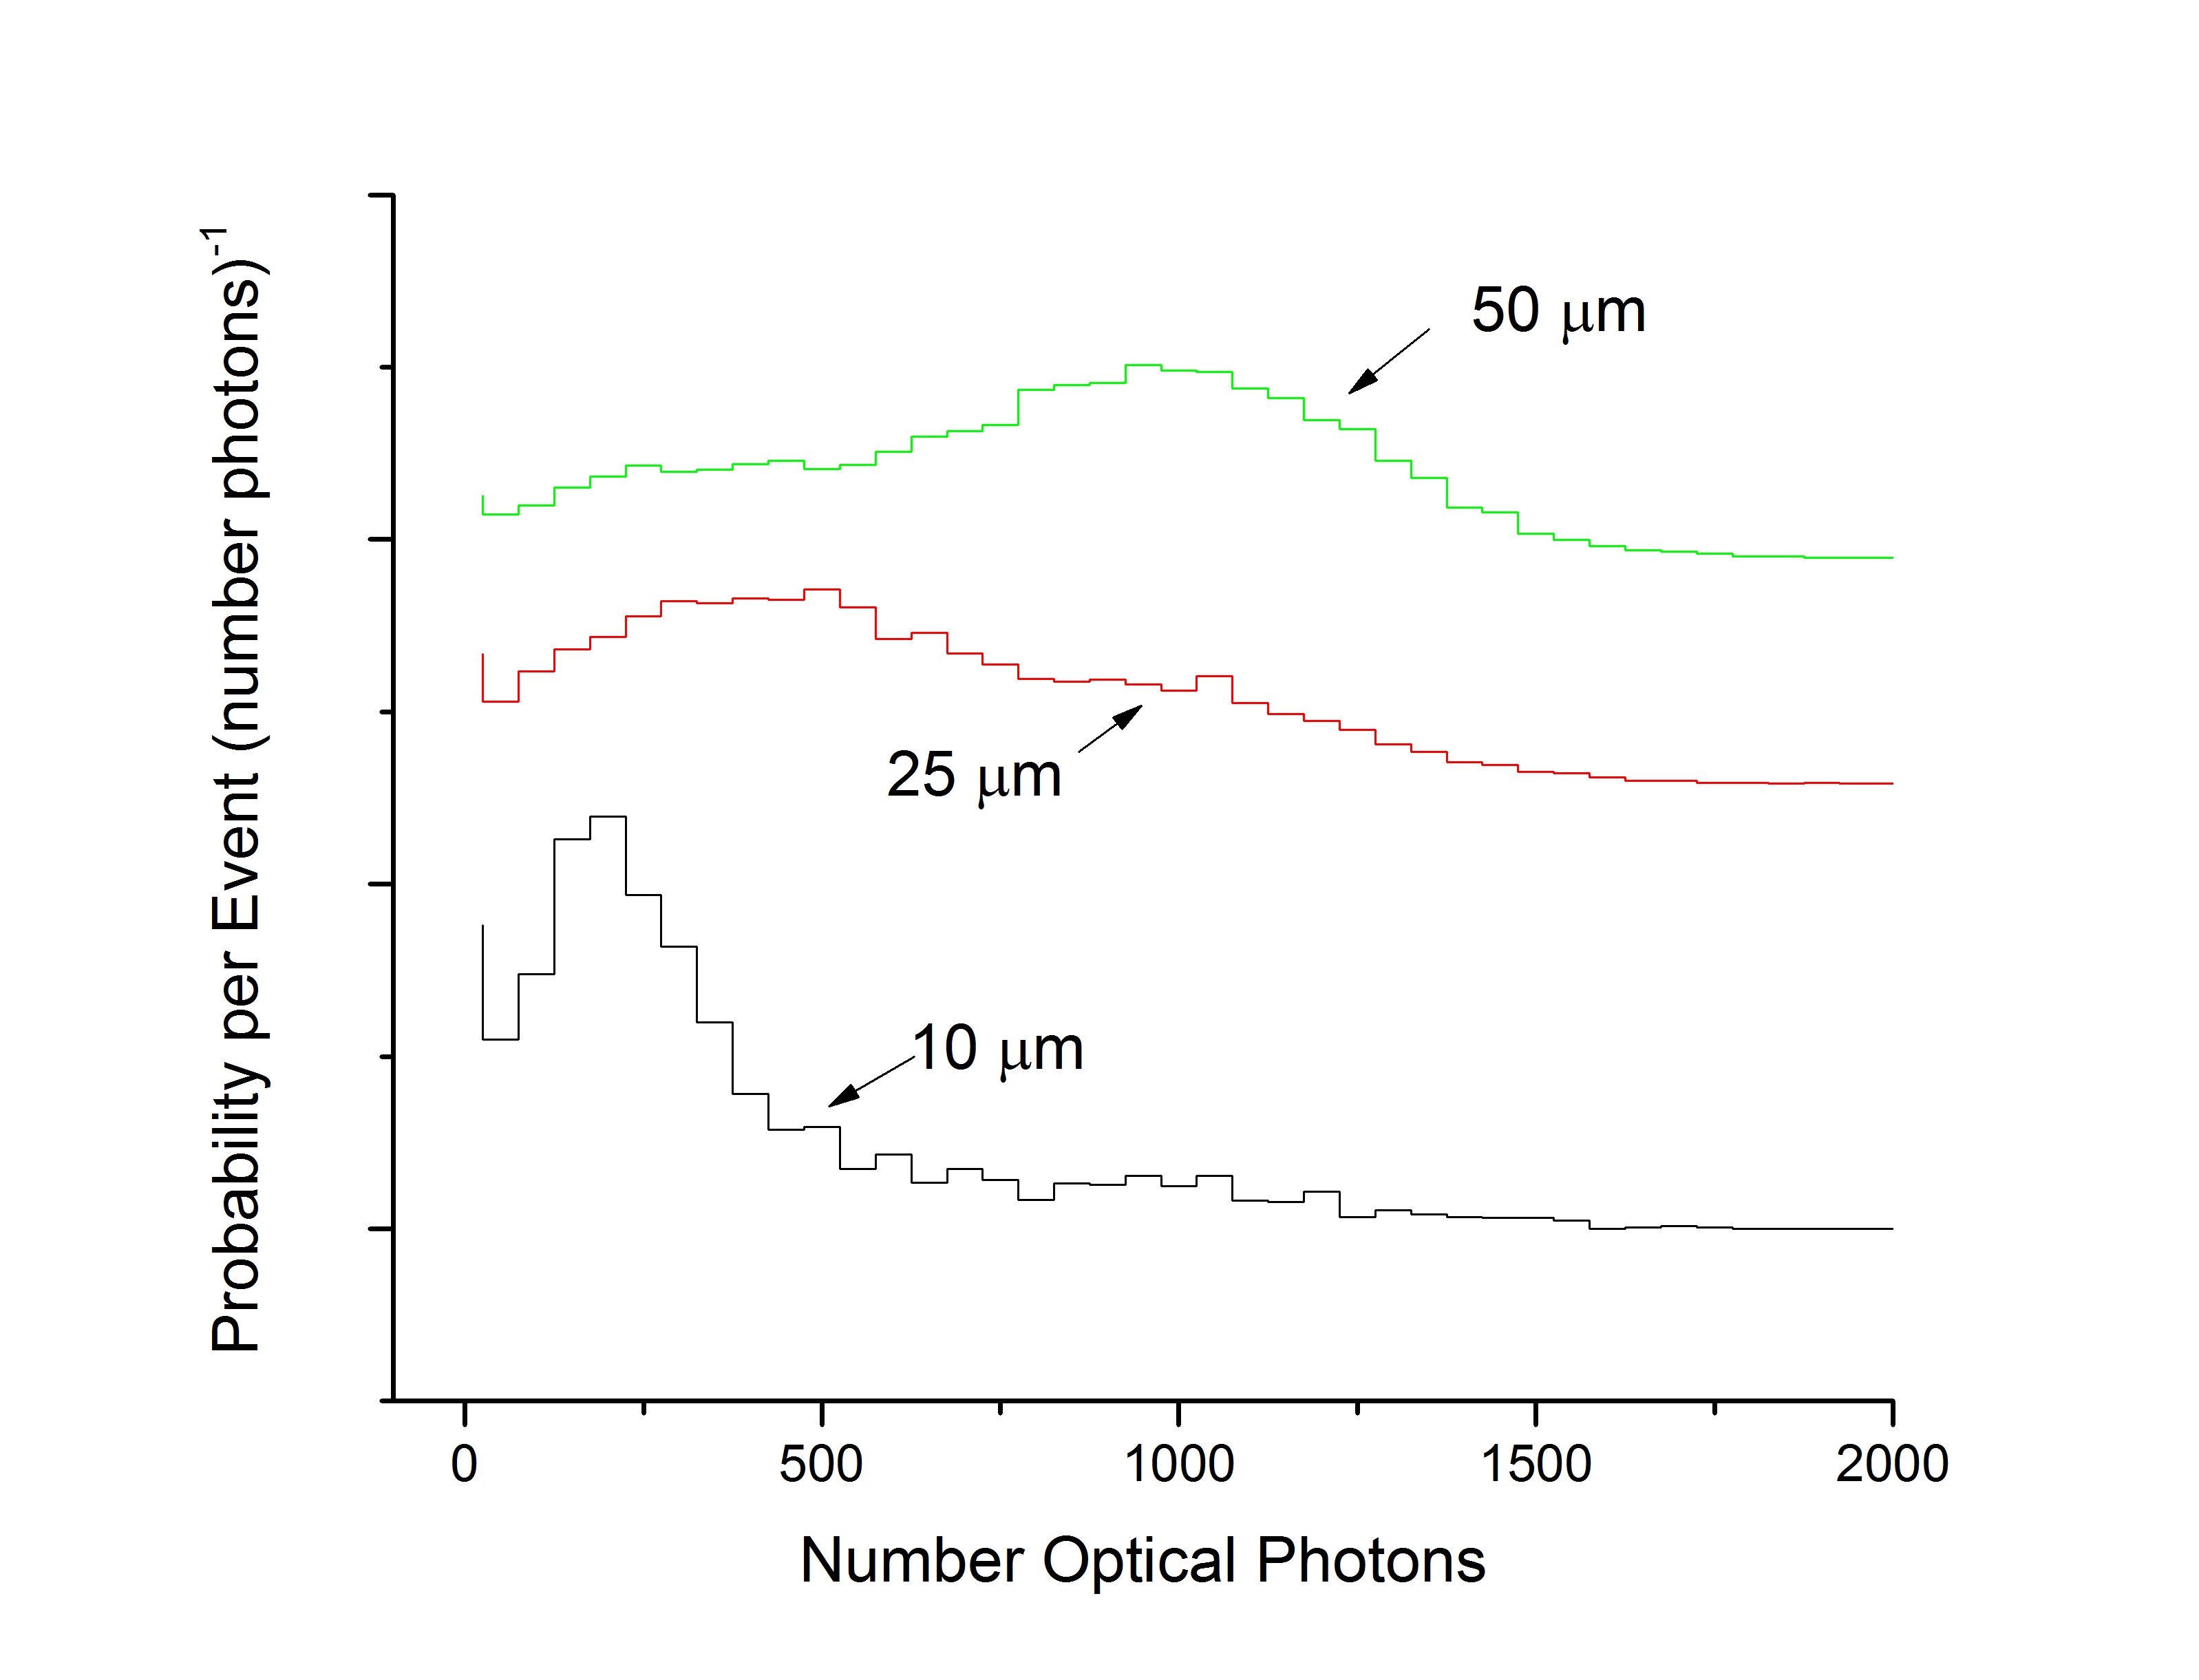
\includegraphics[width=\textwidth]{Neutron_PhotonsGenerated_Sim}
  \caption[Number of photons generated from neutron interactions]{Simulated number of photons generated from neturon interactions.  For the \SI{10}{\um} film it is observed that the majority of the photons are generated by a partial energy deposition corresponding to the alpha paricle, and this effect tappers off as the films get thicker}
  \label{fig:NeutronPhotonsGenSim}
\end{figure}

\begin{figure}
  \centering
  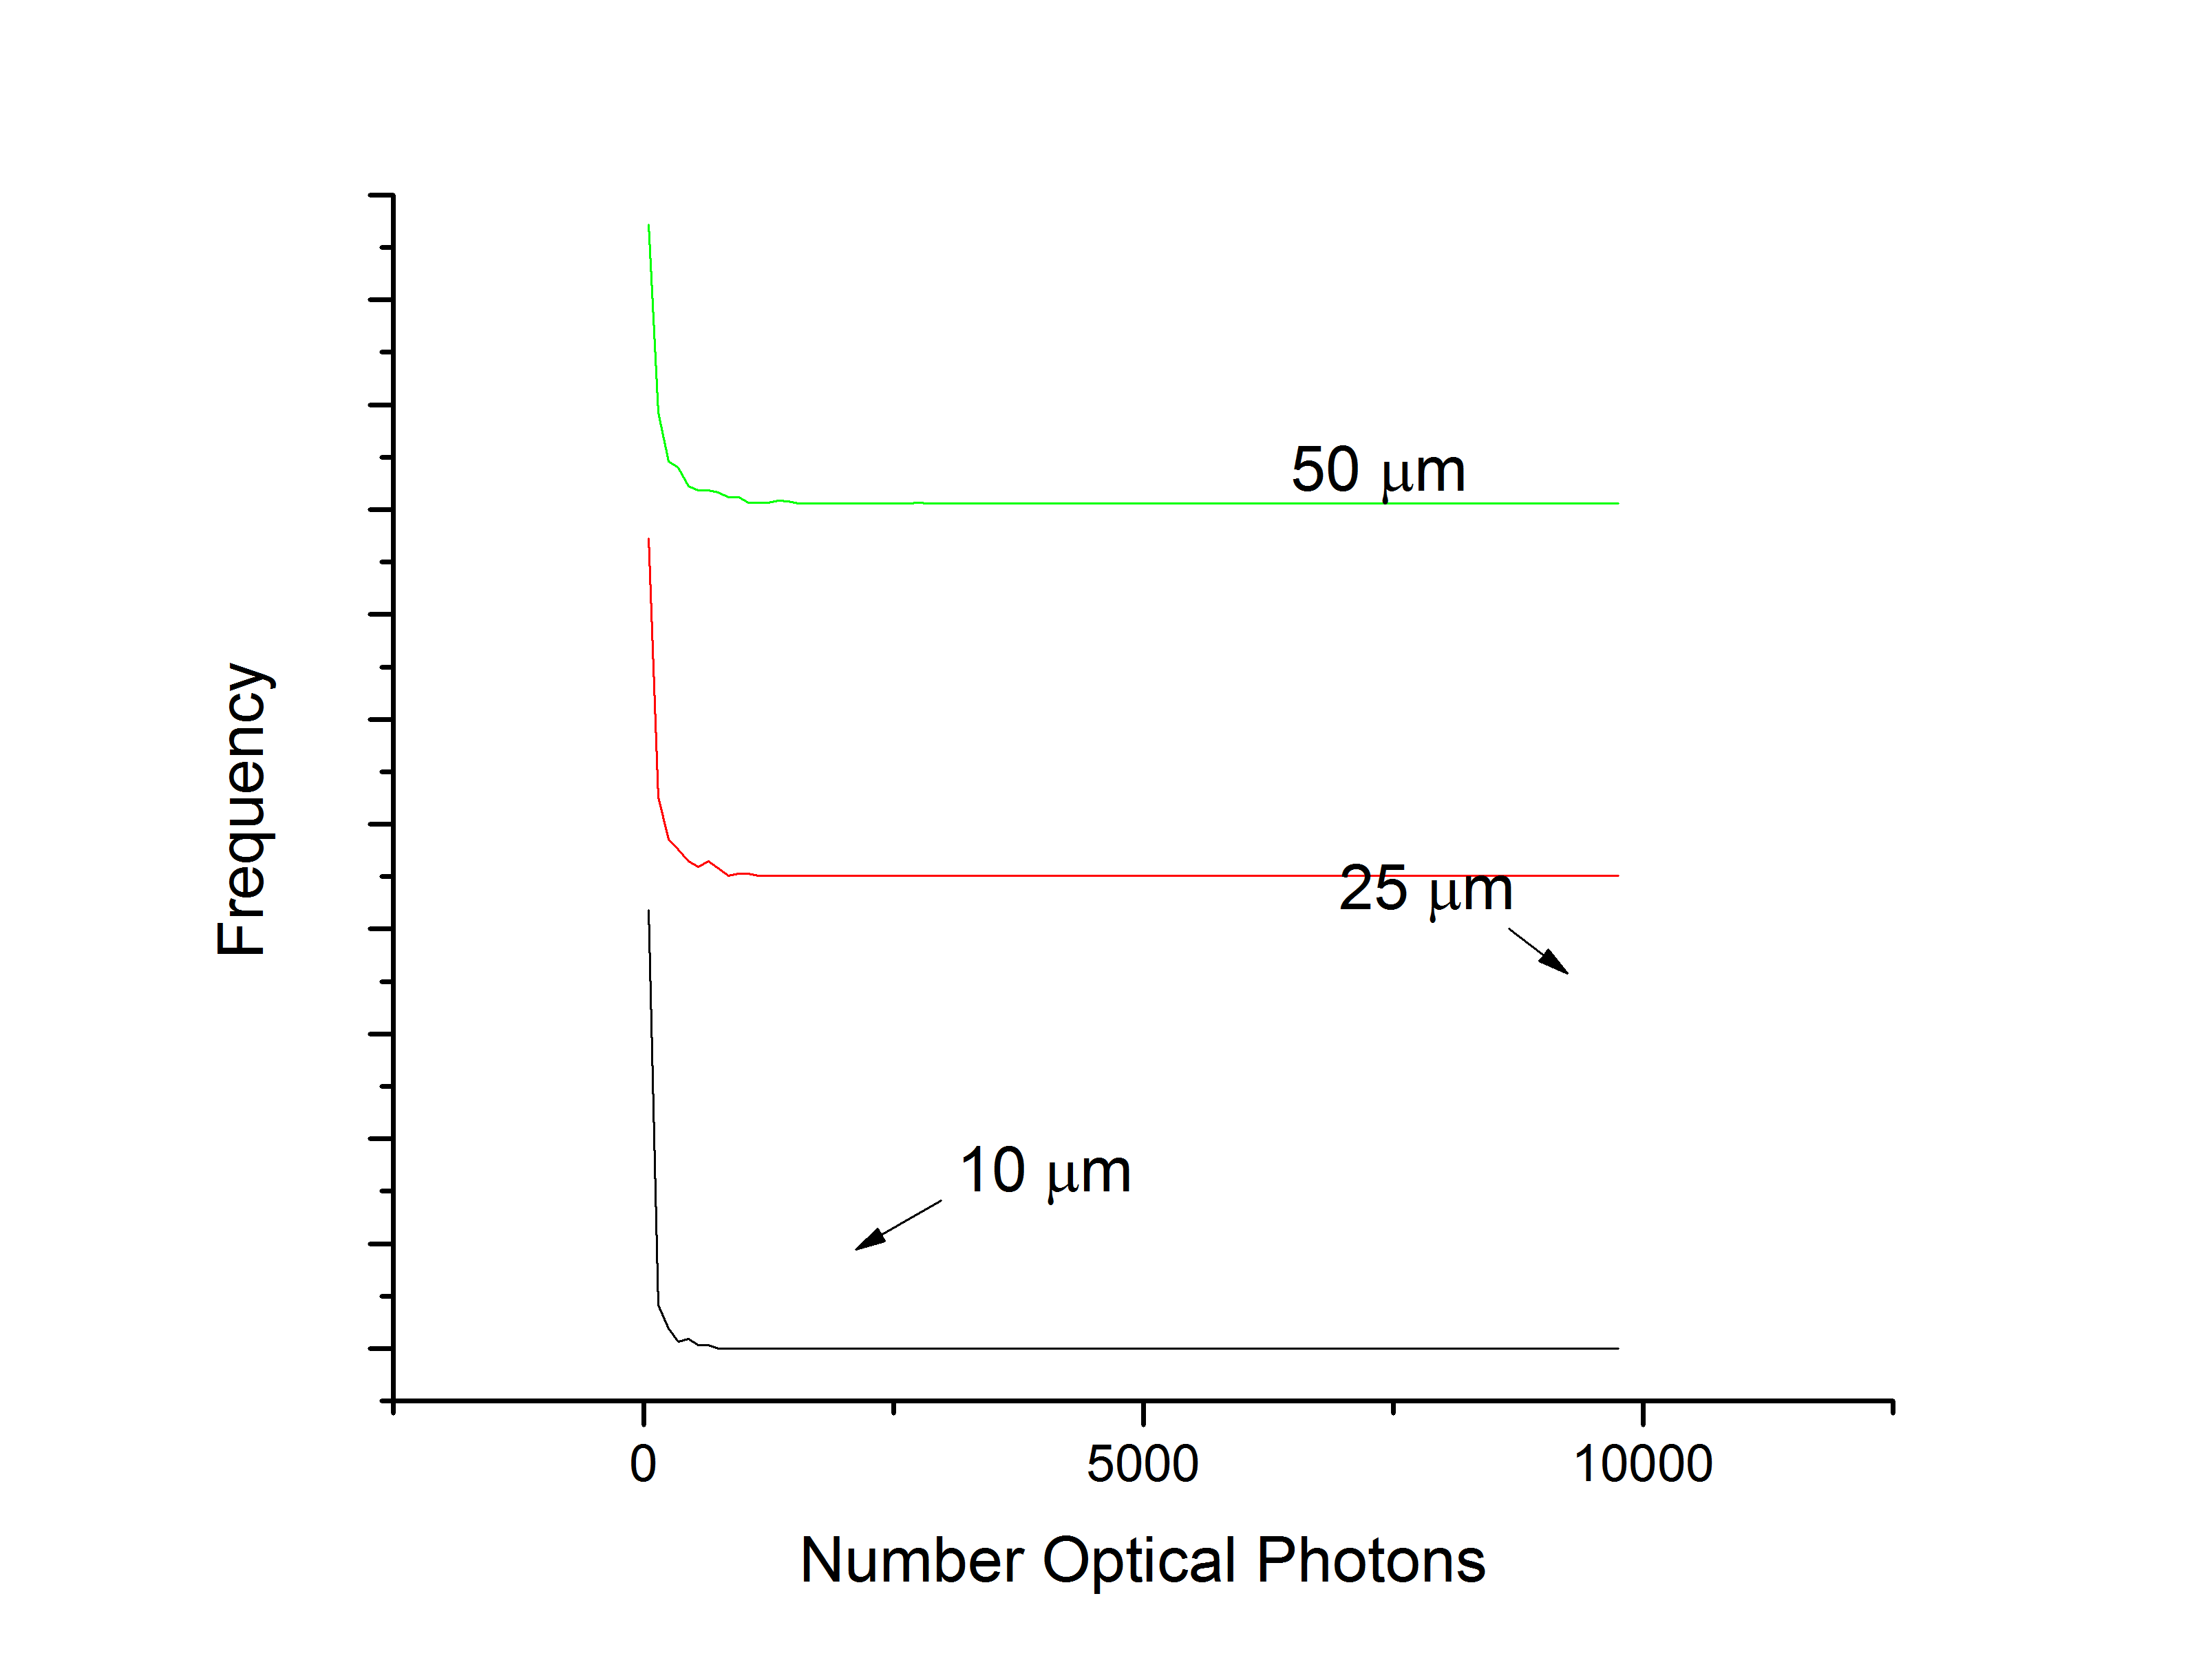
\includegraphics[width=\textwidth]{Gamma_PhotonsGenerated_Sim}
  \caption[Number of photons generated from gamma interactions]{Simulated number of photons generated from gamma interactions.}
  \label{fig:GammaPhotonsGenSim}
\end{figure}

The calculated gamma intrinsic efficiency for six polymeric films along with the neutron response of two of the films in Figure \ref{fig:GammaIntrNeutronCounts}, and the fraction of neutron counts above the MLLD necessary for a given gamma intrinsic efficiency is plotted in Figure \ref{fig:crVsIntEff}.
It is observed that if the films are thin enough (less than \SI{150}{\um}) it is possible to have a significant count rate above the mathematical lower level discriminator necessary for the pulse height discrimination of one in a million.
This is seen by the \SI{50}{\um} film and the \SI{150}{\um} film having the tail of their neutron spectra above the pulse height discriminator necessary for an intrinsic efficiency of \num{1E-6}.
Table \ref{tab:FractionCRGamma} shows the fraction of neutron count rate that is above the MLLD necessary for $\epsilon_{int,\gamma n} \le \si{1E-6}$.
Films less than \SI{50}{\um} have over 2\% of the counts above the necessary discriminator setting, while thicker films have have a factor of 10 less.
\begin{figure}[ht]
    \centering
    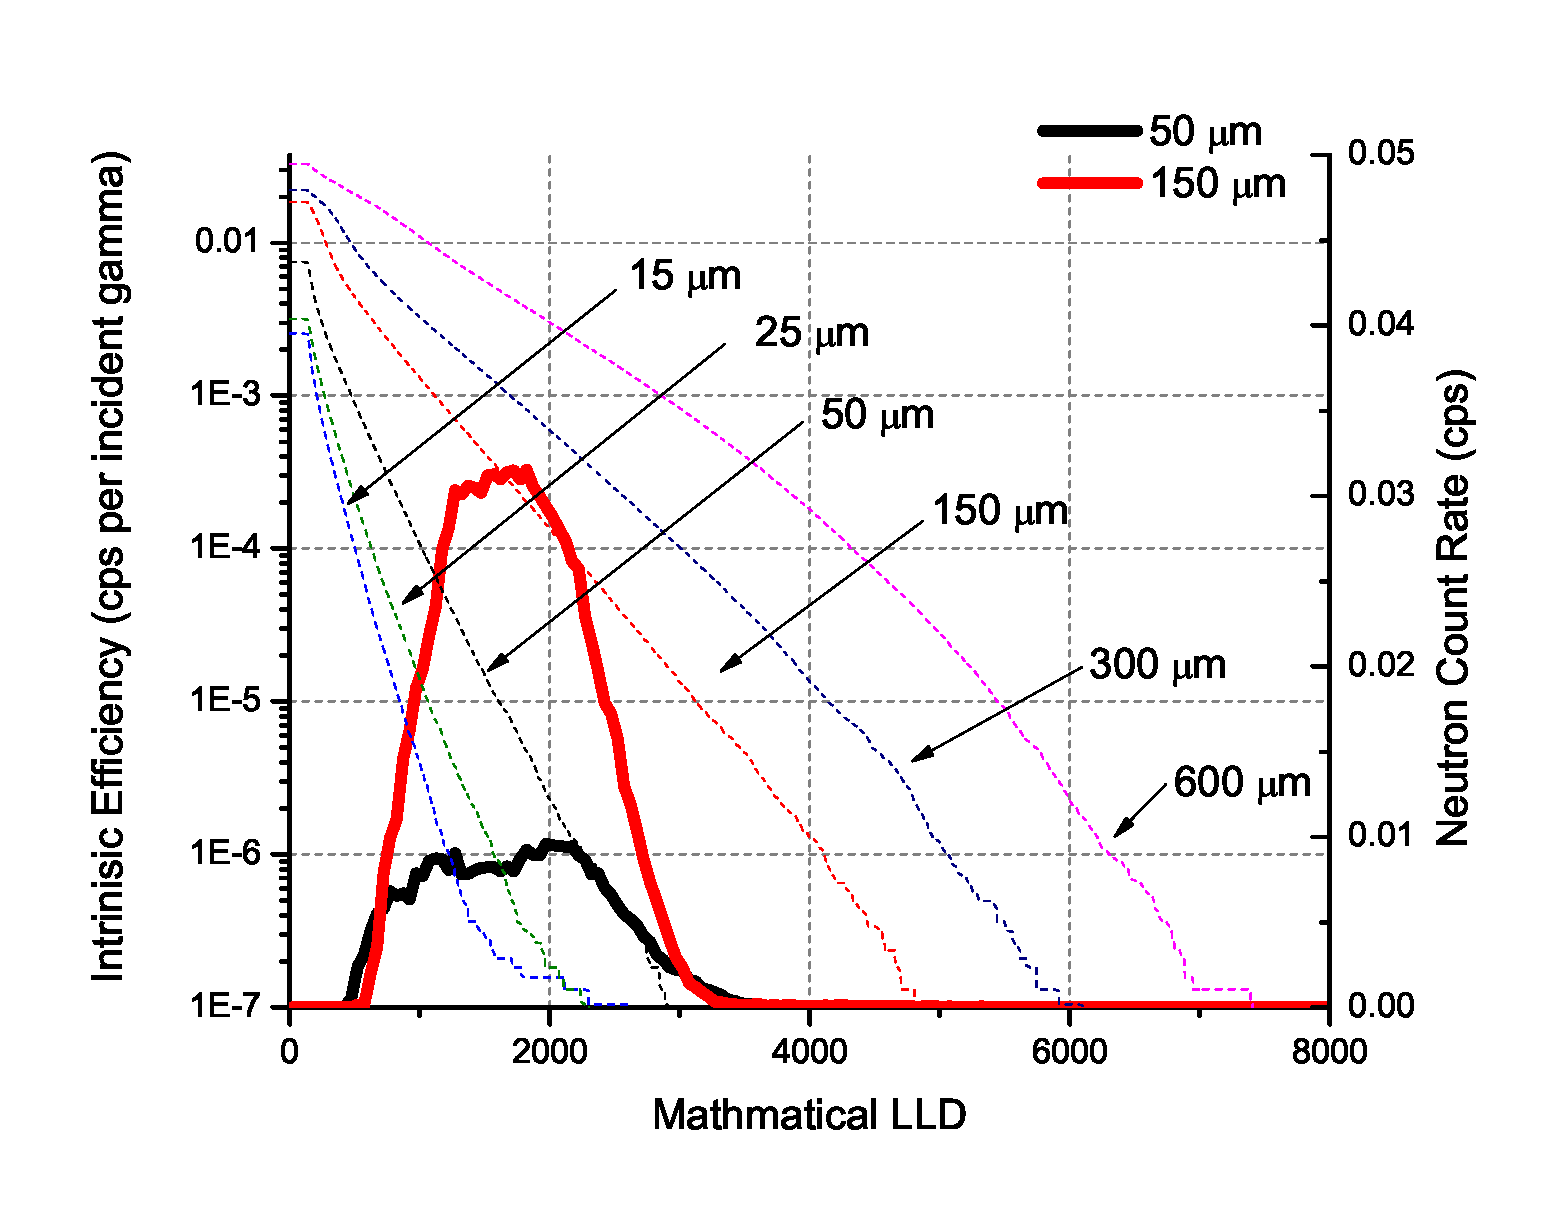
\includegraphics[width=\textwidth]{PS_IntEff_LiF20_PPO5}
    \caption[PS Gamma intrinsic efficiency and neutron count rate]{Gamma intrinsic efficiency (dashed lines) plotted against neutron counts (solid). The gamma spectra has been normalized by the number of incident photons upon the sample, while the neutron spectra has not.}
    \label{fig:GammaIntrNeutronCounts}
\end{figure}
\begin{figure}[ht]
    \centering
    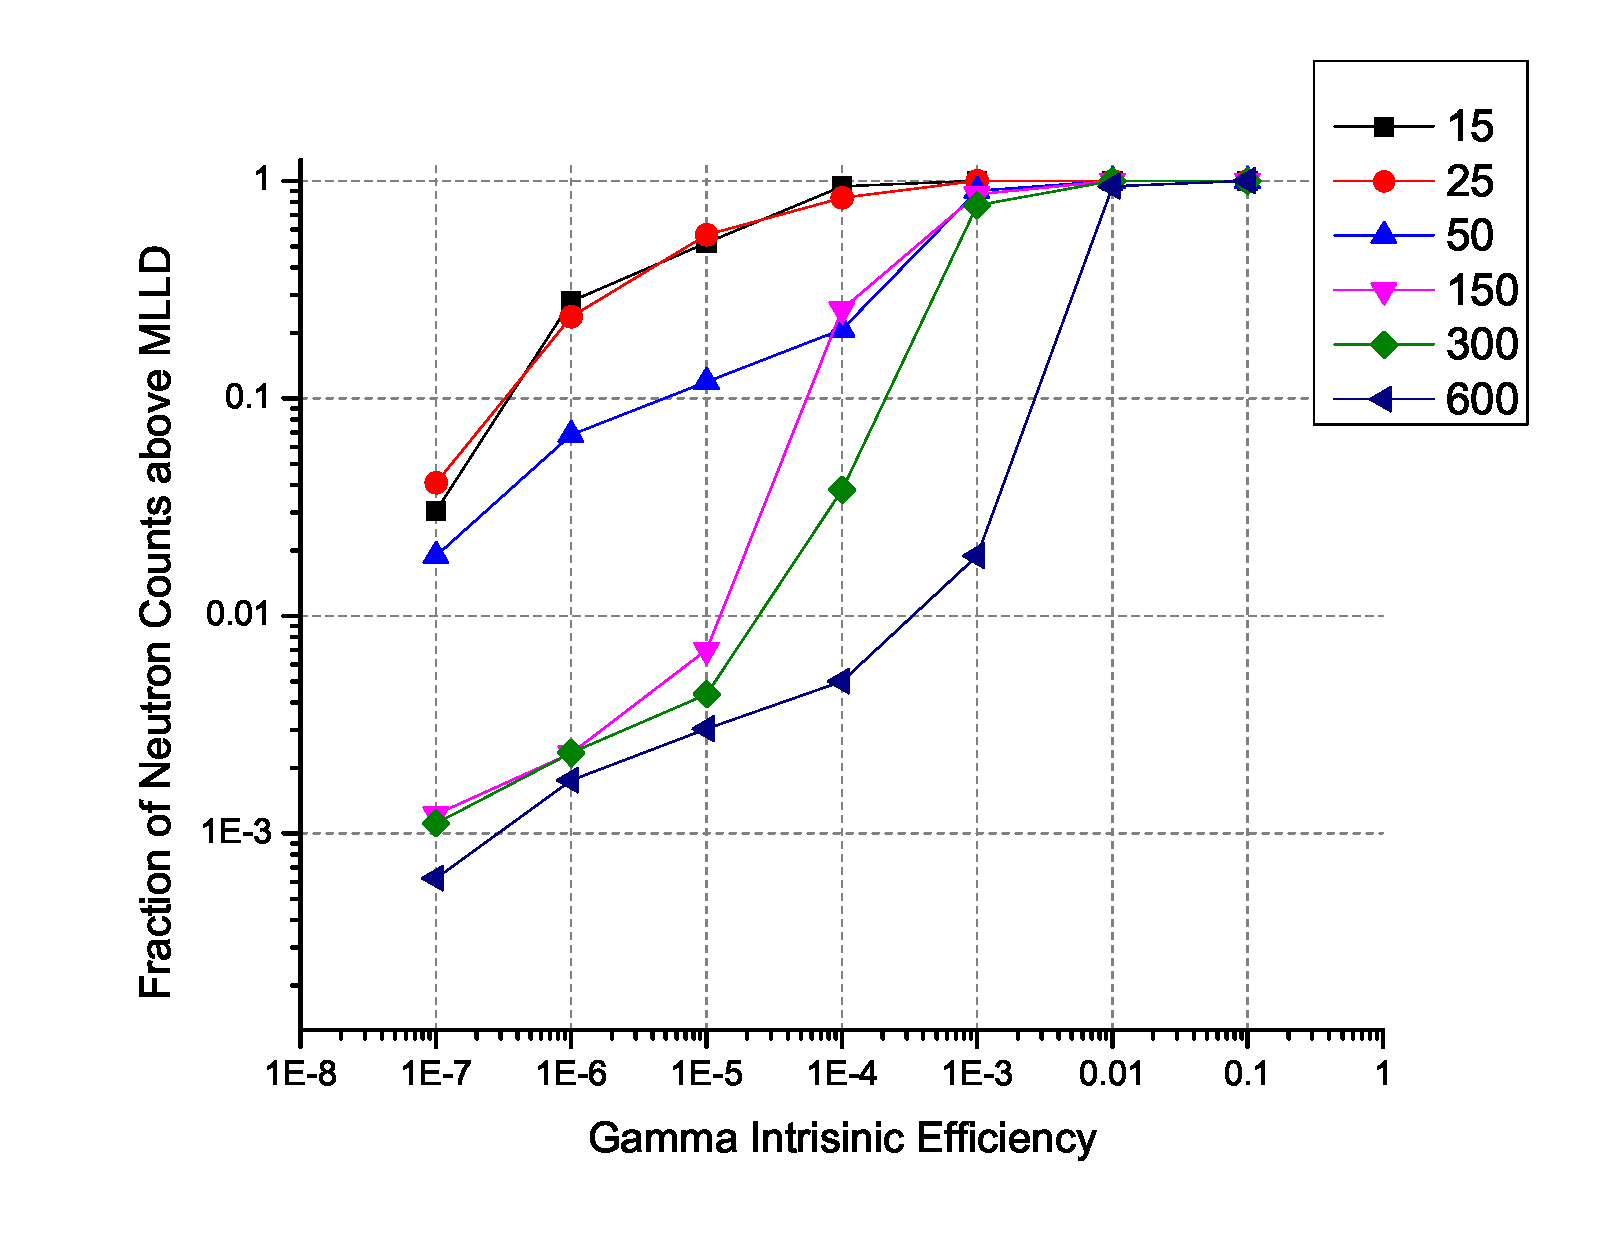
\includegraphics[width=\textwidth]{PS_IntFractionNCR_LiF}
    \caption{Intrinsic efficiency versus neutron count rate. }
    \label{fig:crVsIntEff}
\end{figure}
\begin{table}[]
    \caption{Fraction of Neutron Count Rate Above Discriminator Setting}
	\centering
	\begin{tabular}{c | c}
	Thickness & Neutron Fraction \\
	\hline
	\hline
	\SI{15}{\um} & 0.28 \\
	\SI{25}{\um} & 0.024 \\
	\SI{50}{\um}  & 0.067 \\
	\SI{150}{\um}  & 0.023 \\
	\SI{300}{\um}  & 0.023 \\
	\SI{600}{\um}  & 0.0017 \\
	\end{tabular}
  \label{tab:FractionCRGamma}
\end{table}
In addition it is observed in Figure \ref{fig:GammaIntrNeutronCounts} that for neutrons, thicker films only enhance the resolution of the film and do little to increase the light yield, as most of energy from a neutron event is captured in the film.
The average energy deposited was computed for each thickness and normalized by the incident energy for gammas by the Q-value of the reaction for neutrons, and is presented in Table ~\ref{tab:FractionEDep}.
For thickness greater than \SI{150}{\um} there is little benefit in increasing the thickness of the film in terms of energy deposition by neutrons, since over 90\% of the energy is being deposited in the film.
\begin{table}[ht]
    \caption{Fractional Energy Deposition for Various Thickness}
	\centering
	\begin{tabular}{c | c c}
	Thickness & Gamma Fraction & Neutron Fraction \\
	\hline
	\hline
	\SI{15}{\um} & 0.010 & 0.531 \\
	\SI{25}{\um} & 0.013 & 0.634 \\
	\SI{50}{\um} & 0.017 & 0.782 \\
	\SI{150}{\um} & 0.032 & 0.927 \\
	\SI{300}{\um} & 0.052 & 0.964 \\
	\SI{600}{\um} & 0.087 & 0.982 \\
	\SI{1}{\mm} & 0.130 & 0.989 \\
	\SI{1}{\cm} & 0.425 & 0.998 \\
	\end{tabular}
  \label{tab:FractionEDep}
\end{table}

Figure \ref{fig:simKinE} illustrates the simulated kinetic energy of secondary electrons from Compton scattering and from alpha and triton interactions.
It is observed that kinetic energy of the secondary electrons from the neutron reaction products have predominately energies in the kilo-volt range, while the Compton scattering electrons have energies in hundreds of kilo-volts range. 
However, it should be noted that there is only one secondary electron from a Compton scattering and multiple secondary electrons from the reaction products.
Figure \ref{fig:ReacProdDist} shows the distribution of the number of secondary electrons from the alpha and triton and their kinetic energy.
\begin{figure}[ht]
    \centering
    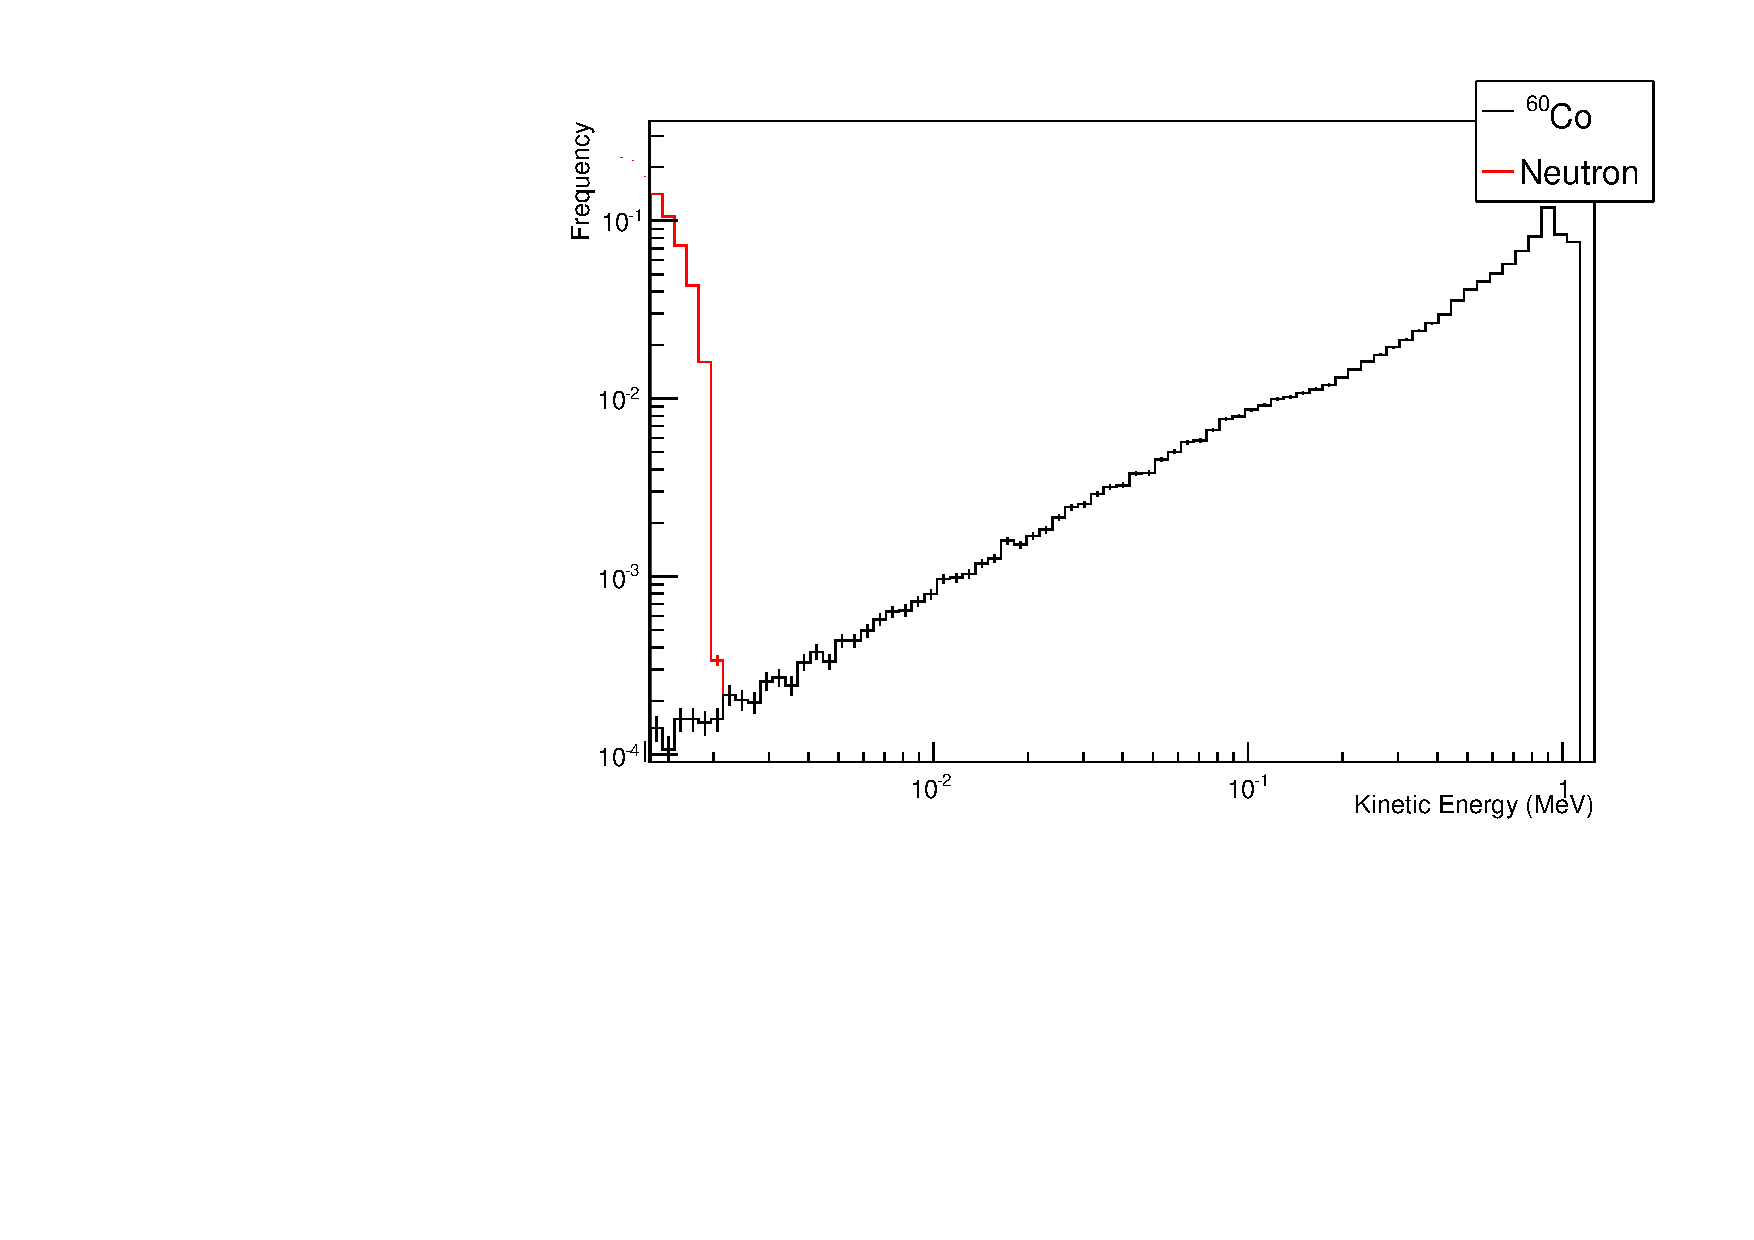
\includegraphics[width=\textwidth]{NGSecElecKinEDist}
    \caption{Simulated Kinetic Energy of Secondary Electrons from Compton Scattering and from \iso[6]{Li} reaction products}
    \label{fig:simKinE}
\end{figure}
\begin{figure*}[ht]
	\centering
	\begin{subfigure}[b]{0.45\textwidth}
    		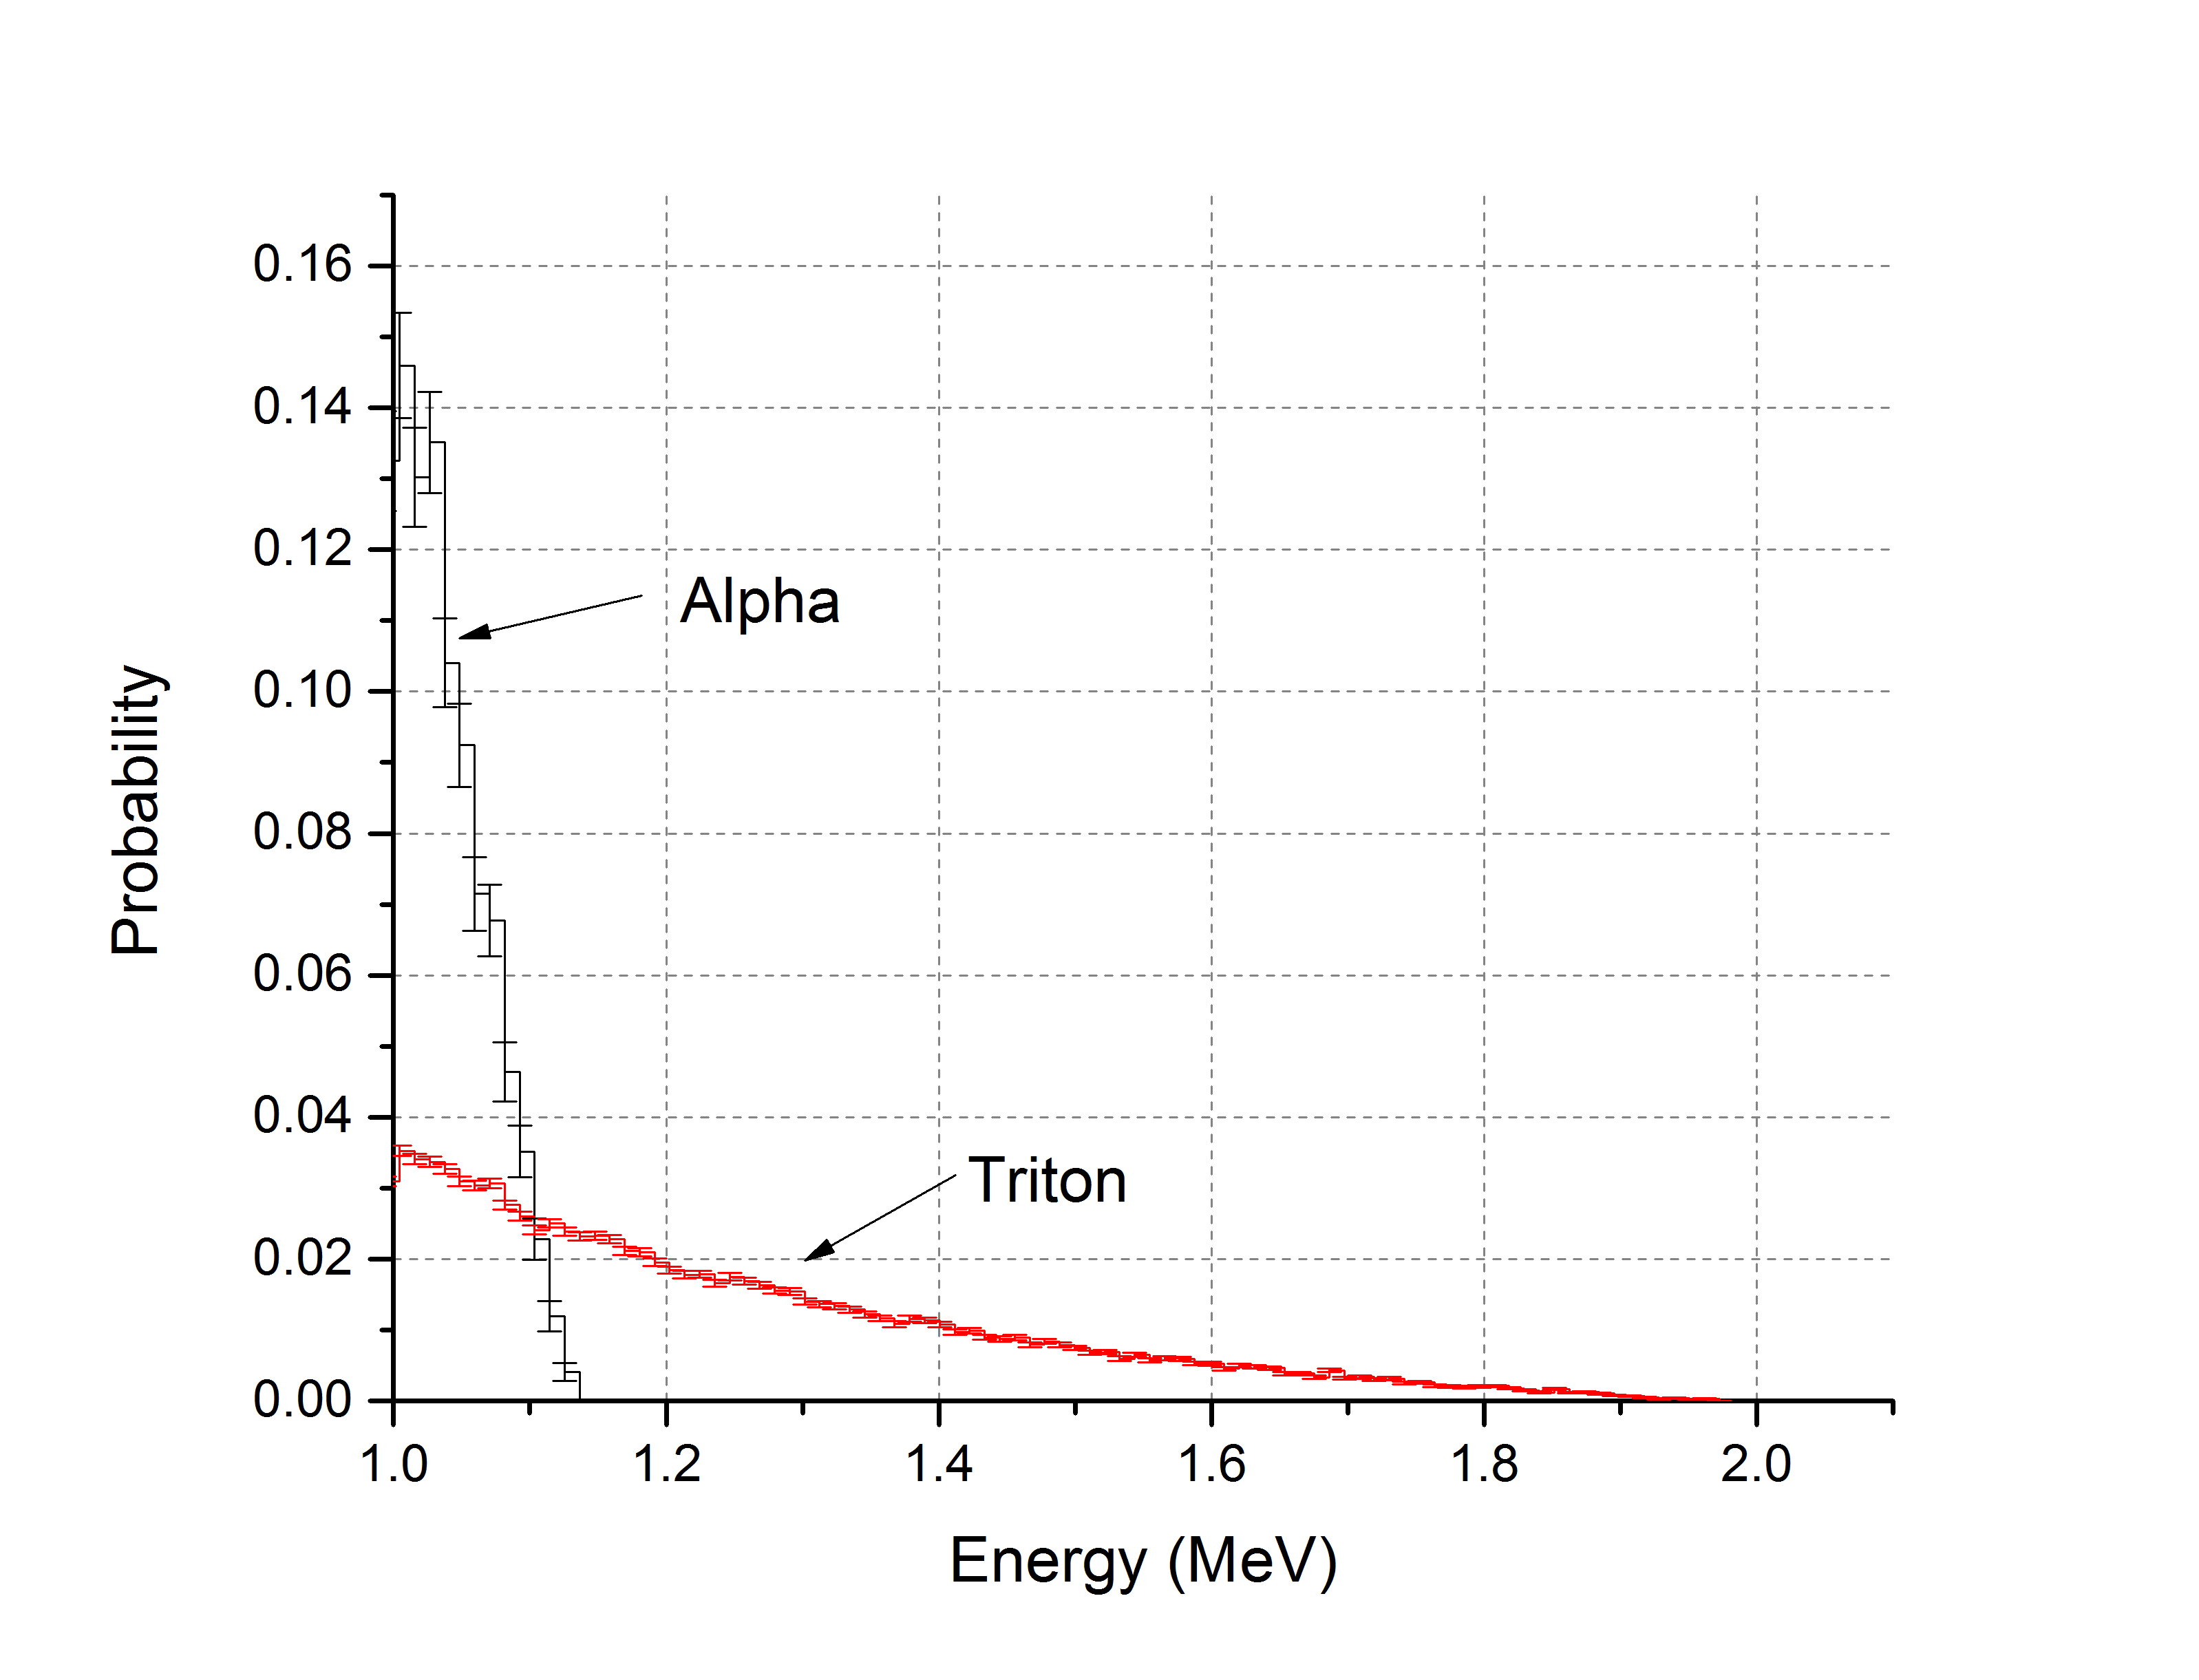
\includegraphics[width=\textwidth]{AlphaTritonSecElecKinEDist}
		\caption{Alpha and Triton Secondary Electron Kinetic Energy Distribution}
	\end{subfigure}%
	~
	\begin{subfigure}[b]{0.45\textwidth}
    		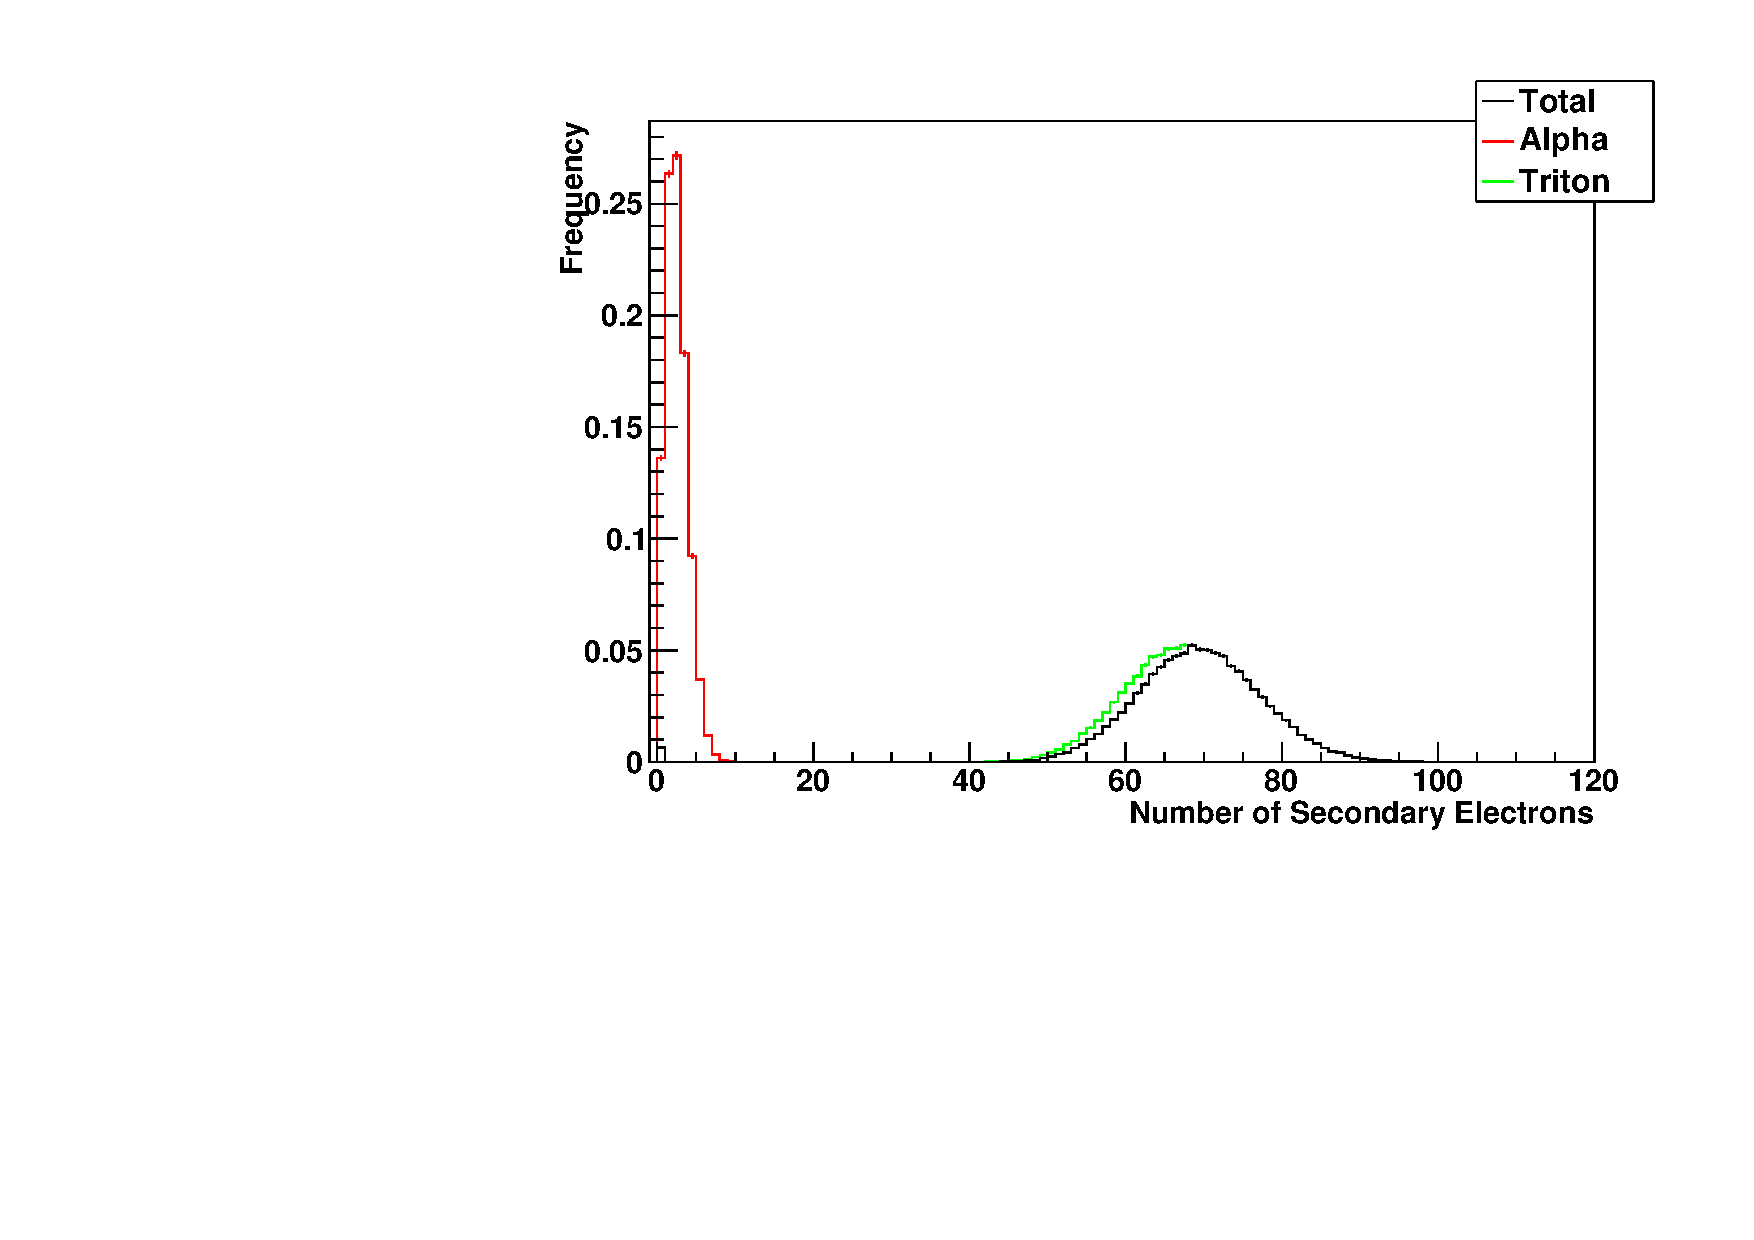
\includegraphics[width=\textwidth]{NeutronNumSecElec}
		\caption{Number of Secondary Electrons Produced Per Neutron Interaction}
	\end{subfigure}%
	\caption{Neutron Reaction Products Secondary Electrons Energies}
	\label{fig:ReacProdDist}
\end{figure*}
  
    \chapter{Neutronic Optimization}
\label{ch:GAOpt}
\section{Introduction}
Effective utilization of the neutron flux and is necessary for minimizing the amount of neutron absorber (\iso[6]{Li}) that is used in the detector.

Several possible geometries have been considered for the films. 
They are generally a vertical or horizontal layer of the films or a vertical or horizontal arrangement of the films arranged in concentric cylinders.
\section{Methods}

%%%
A fast simulation model (XSDRN) will be used to preform an initial parameter study and determine a subset of optimal geometries on which to preform more accurate Monte Carlo (MCNPX) modeling. 
A subset of the highest preforming geometries validated by the detailed model with then be used to test the sensitivity by adjusting the position of the films by fractional amounts.
%%%
\subsection{Genetic Algorithm Introduction}
Genetic algorthims provide a search technique analagous to biological evolution in which instead of searching from general to specific solutions, or from more simple to complex, genetic algorthims generate solutions by mutating and combining parts of the best previously known solutions.
At each step in the search for the best solution a collection of solutions called the current \textit{population} is refined by replacing members with solutions representing the offspring of the best individuals.
The goals is then to find the best solution to the problem as determined by some criteria, called the \textit{fitness function}.
The genetic algorithm typically consist of four tasks: creating an initial population, evaluating that populations fitness, selecting members of the current population to breed, and then applying genetic operators to the selected members to breed the new population. 
This is completed until either a maximum generation is reached or the desired fitness is achieved, as shown in \autoref{alg:GAOutline}.
\begin{algorithm}
  \caption{Genetic Program Outline}
  \label{alg:GAOutline}
  \begin{algorithmic}
    \WHILE{$error>goal$}
      \FORALL{$t\in F$}
        \STATE{Compute fitness}
      \ENDFOR
      \FORALL{$t\in F$
        \STATE{Choose individuals based on fitness}
      \ENDFOR
      \STATE{Select individuals for next population}
      \STATE{Crossover selected individuals}
      \STATE{Mutate selected individual}}}
    \ENDWHILE
  \end{algorithmic}
\end{algorithm}

First, however, it is necessary to become familar with the terms used in genetic programming.
\begin{itemize}
  \item \verb+genome+ The set of all genes of an individual, where a gene is a problem parameter.  The problem representation
  \item \verb+population+ All individuals that represent a solution to the problem at a given point in time
  \item \verb+selection+ Choosing which individuals go on to produce new offspring
\end{itemzie}
\subsubsection{Initial Population}

The inital population


\subsection{Population Selection}

Population selection was achieved using a hybrid approach of tournament
selection and rank selection. In rank selection the individuals were
selected based on their rank, where the rank was determined by their
fitness (lower SSE correspond to a higher fitness). Tournament selection
was used to generate the other component of the population for breeding.
\subsection{Genetic Operators}

Individuals selected for reproduction are subjected to genetic operators
to breed the next generation. Genetic programs generally contain two
genetic operators, crossover and mutation. Crossover serves to create
new members of the population by interchanging the genetic material
(tree structure) of two parents in which significant changes in the
tree solutions are achieved. Mutation serves to slightly modify an
existing solution. 


\subsubsection{Crossover}

Crossover is defined in genetic programming as the swapping of sub-trees
between individuals in the population, which is meant to mimic the
crossover of genes that occurs during evolution. As the solutions
are recursively defined, crossover was implemented by selecting randomly
selecting a two nodes from different trees and swapping their parents.


\subsubsection{Mutation}

Mutation, unlike crossover, does not involve changes to the structure
of the solution but rather operators within the solution. For example,
in symbolic regression mutation will randomly (defined by the mutation
rate) change the node function and leaf values, but it will not add
or prune branches to the tree structure. Mutation was implemented
as a recursive traversal of the tree, switching the function types
with other functions types according to a user supplied probability.
The terminals mutations were implemented in a similar fashion, but
if the node was a value leaf the leaf was randomly set to a new random
variable. An example of mutation is shown in Figure \ref{Mutation}.

\subsubsection{Selection Techniques}
Several differnet selection technqiues are available to select the individuals from one population to reproduce in the next.
Among the most common are fitness proportional selection (roulette selection) and tournament selection.

Fitness proporitional selection (or roulette selection) occurs when the individuals are ranked by their fitness, and individuals are chosen by their fitness rank.
Imagine a roulette wheel where the space a canidate occupies on the wheel is proporitonal to its fiteness.  
Higher fitness individuals will occupy more space, and will thus have a higher probability of being selected.

Roulette selection avoids some of the local minima by providing an opertunity for less fit individuals to be selected.

% MCNPX Model of the interaction rate
The performance of films is simulated in MCNPX, a Monte Carlo transport code\cite{pelowitz_mcnpx_????}.
The geometry is as in the PNNL reports, namely a nano-gram of \iso[252]{Cf}  encased in \SI{0.5}{\cm} of lead and \SI{2.5}{\cm} of HDPE. 
The size of the RPM8 is \SI{12.7}{\cm} deep, by \SI{30}{\cm} wide and \SI{2}{\m} tall.
The interaction rate, $I_{\text{sim}}$ provides the total number of simulated neutron interactions in the detector and is calculated using the a cell flux tally in MCNPX and a tally multiplier card.
The reaction rate $\iso[6]{Li}\left(\text{n},\text{t}\right)\alpha$ can be calculated by then applying the appropriate input for the FMn card and using an F4 card to calculate $\phi(E)$.
This is in accordance with the direct evaluation of the PNNL criteria, which require a absolute neutron count rate of \SI{2.5}{count\per\second\per\nano\gram\iso[252]{Cf}}.
Note that in this calculation the source strength is set to be \SI{1}{\nano\gram} \iso[252]{Cf}, which has a neutron emission rate of \SI{2.3E3}{neutron\per\second}.
\begin{align}
  \label{eqn:RPM8InteractionRate}
  I_{\text{sim}} &= S_0 I \\
  &= \SI{2.3E3}{neutron\per\second} I
\end{align}



However, not all of these interactions will lead to counts above the pulse height discriminator setting necessary for meeting the gamma intrinsic efficiency.
This is corrected for by scaling $I_{\text{sim}}$ by the fraction of counts, $\eta$, that occur above the gamma LLD \eqref{eqn:FractionOfCountsDefination}, \eqref{eqn:RPMCountRate}.
\begin{align}
  \label{eqn:FractionOfCountsDefination}
  \eta \equiv \frac{\int_{MLLD}^\infty p(x)dx}{\int_0^\infty p(x)dx}
\end{align}
\nomenclature{$p(x)$}{Measured spectra, as a function of channel number}
\begin{align}
 \label{eqn:RPMCountRate}
 \text{Count Rate} &= I_{\text{sim}} \eta
\end{align}

% XSDRN Model of the RPM
\subsection{XSDRN Detector Model}
The XSDRN model was a simplified model of the RPM along an axis through the midpoint of the RPM.
A $S_n$ of 16 was used for the quadrature, and convergence for the flux was set at \SI{1E-7} for the inner iterations.
Only two types of materials were simulated in the XSDRN calcualation; a detector material containing the \iso[6]{LiF} and a moderating material of polystyrene.
The 44 group neutron cross sections of each of these materials were processed using NITWAL (without any resonance regions) assuming an infinate, homogenous medium for simplicity.
The XSDRN model consisted of a multi-group isotropic boundary source on the left most boundary on the RPM, with the values for this flux coming from an MCNPX simulaiton.
A MCNPX calculation was used to determine the neutron flux incident upon the left most side of the RPM, and then this flux was input as the surface boundary flux condition in XSDRN.

%The XSDRN model was validated by comparing to the MCNPX simulations of a similar geometry.
%It was observed that geometries that started with a neutron absorber layer did not have good agreement with the MCNPX model; this is attributed to the breakdown of the diffusion equation in a strongly absorbing medium near a source.
%Some strification of the results were also observed, leading to the conclusion that the XSDRN calculations should only be used as a general guide.



Further refinement of the spacing could be completed in the MCNPX calculations by adjust the slices a millimeter to the left or right for each one.

\section{Conclusions}

A physical basis of the optimal solution found by the genetic algorthim can be found by observing the form of the optimal solutions.
These solutions involve an intial moderator layer in order to ensure that all of the neutrons are thermalized to (increasing the thermal fraction by \textbf{SOME PRECENT}).
After this moderator layer a film layer is placed to utilize this neutron spectra; however not all of the thermal neutrons are captured (as the mean free path of a neutron in polyethylene is about \si{0.37}{\cm} and thus some pass through the material) and another abosrber layer is needed to capture those neutrons.  
The neutron flux is then moderated again, and additional layers of detectors are needed to capture this neutron cross section.
However, it is desirably to have a large neutron reflector in the portal monitor to reflect neturons back into the detector slices. 
Theortically this reflector should be as large as possible, but the limited space of the RPM provides a constraint.
A parameter study with a single detector slice between a moderator and reflector constrained by the radiaiton portal monitor design showed that it is desriable to have around \textbf{So much} moderator leaving the majority of the RPM to be left for the reflector.
Thus it is demonstrated that a large reflector is desired.

    

\chapter{RPM Light Collection}
\label{chap:LightTransport}
\section{RPM Light Collection Performance}
\label{sec:RPMLCP}



\subsection{Proposed Work}
It is proposed to simulate the neutronics, energy deposition, and light transport and collection of the optical photons with the GEANT4 toolkit to ensure that the proposed detector designs will be feasible. 
This will then have two parts:
\begin{enumerate}
  \item the fabrication and simulation of detectors whose performance can be measured in the laboratory, and
  \item the simulation of a RPM in the geometry specified by the neutronics calculations.
\end{enumerate}
It is also proposed to explore the design space of the light collection instrumentation, where such design options include
\begin{itemize}
  \item the use of a wavelength shifter (WLS) to increase the detected optical photons by decrease the optical photons absorbed in the light guide,
  \item the design of a light guide to enhance the photons reflected towards the PMT,
  \item the application of different light reflection techniques (air gap, Teflon tape, aluminized mylar) to enhance the light collection, and
  \item the placement of PMT's for their effective utilization.
\end{itemize}
The developed GEANT4 application will then have the ability to fully simulate the performance of a replacement RPM.

\subsection{Methodology}
The full simulation of the light transport of the RPM will be completed in with the GEANT4 toolkit.
GEANT4 offers three example simulations for generation and tracking of optical photons (\verb+ExampleN06+, \verb+extended/LXe+, and \verb+extended/WLS+).
These examples will be adapted for the purposes of this simulation.
However, it should be noted that the \verb+LXe+ and \verb+WLS+ utilize a sensitive detector which kills tracks, and for the purposes of the simulation of the RPM this will not be implemented.

The validation of the GEANT4 simulations will be completed with the fabrication of a 4 inches by 6 inches layered detector to allow the toolset to be benchmarked against measurements.
Detectors of various materials (boron loaded plastic, lithium loaded polymers, and LiF/ZnS(Ag)) will be tested to avoid a basis in the simulation parameters.
Where possible, the optical parameters of the materials will be taken from the literature.
However, it they cannot be found a similar material for which the property is know will be substituted.
In addition, rather than providing reflectivity parameters for each material, a model of optical surface will be used according to the work of Janecek\cite{5485130}. 

The GEANT4 light transport simulation code base will be written such that bit-string geometries from genetic algorithm optimization can be directly implemented.
With this formulation it will be possible to reuse the genetic algorithm optimization code base, while additionally providing a validation of the GEANT4 neutronic calculations against the MCNPX.

    \chapter{Conclusions}
\label{chap:Conclusions}
Defense against nuclear terrorism relies upon the ability to accurately detect and identify Special Nuclear Material (SNM).
The current standard for neutron detection in portal monitors is \iso[3]{He}, which is a diminishing resource. 
A significant amount of research is then focused on developing new (or optimizing an existing) neutron detection system to serve as a replacement RPMs.

Thin (less than approximately \SI{150}{\um}) polymeric films loaded with \iso[6]{Li} films or \iso[6]{Li} loaded ZnS:Ag scintillators show promise in meeting the criteria for replacement detectors; namely a 1) neutron interaction rate greater than 2.5 per nanogram \iso[252]{Cf} (in a specified test configuration) 2) an intrinsic gamma ray detection efficiency of less than one in a million in a 10 mR/hr field, and 3) the neutron and gamma efficiencies should not change by more than 10\% in a 10 mR/hr gamma field.
Design of a replacement detector technology capable of meeting these criteria needs to account for neutron interaction used for detection, the subsequent energy deposition  of the reaction products into the material, the scintillation that results from the energy deposition, and the transport of photons from the interaction site to the photomultiplier tube.
Understanding these complex reactions involve understanding the mechanisms of scintillation, light transport, and energy deposition while developing techniques to confirm simulations and confirm the light yield,intrinsic efficiency and count rate for the different detector materials.

\section{Neutron - Gamma Discrimination}
This work presented in this thesis outlines an approach in which a detector material is first characterized for it's ability to meet a gamma ray detection efficiency of less than one in a million. 
A pulse height discriminator is implemented as a mathematical lower level discriminator (MLLD) in which counts that are above a given channel number are counted as neutron counts, and counts below are discarded.
MCNPX simulations where used to establish the photon fluence over samples mounted on a PMT exposed to a 10 mR/hr field, allowing for the count rate per particle crossing to be established.
The MLLD is then determined as the discriminator setting in which for every million photons that cross the detector only one is counted.

The origination of the neutron - gamma discrimination in primary in film thickness as the scintillators tested for replacement detector criteria are low - z materials.
The thickness of the film impacts the discrimination firstly through the interaction rate, but a far greater impact on the neutron - gamma discrimination comes from the range of the secondary electrons produced by Compton scattering in gamma-photon events and their energy deposition.
The electrons from the gamma interactions generally have energies on the order of 100 keV, while energies from the charged particle reactions of the neutrons have energies or the order to 10 keV.
Thus, the neutron reaction product energies tend to deposit more energy in the film than their gamma produced counterparts.
It is the poor energy deposition by electrons generated from photon events that allow for films to be much thicker than the thickness predicted based on the interaction rate.

Effective design must account for the energy deposition in the material, including the pulse height deficit of the impingement particle.
For example, the range of the alpha created in a \iso[6]{Li} neutron absorption is six times less than that of the triton, but the triton creates almost six times more photons than the alpha.
Simulations were completed using the GEANT4 toolkit to simulate the energy deposition of \iso[6]{LiF} loaded polystyrene
For thickness greater than \SI{150}{\um} there is little benefit in increasing the thickness of the film in terms of energy deposition by neutrons, since over 90\% of the energy is being deposited in the film, thus there is little reason to fabricate films thicker than \SI{150}{\um} because it allows for a greater percentage of energy to be deposited from gammas, resulting in a higher MLLD setting.

\section{Film Placement}
A single film does not have an adequate neutron count rate to satisfy the neutron detector requirements of 2.5 cps per nanogram \iso[252]{Cf} in a source that is \SI{2}{\m} from the detector midpoint, shielded by \SI{0.5}{\cm} of lead and moderated by \SI{2.5}{\cm} of high density polyethylene.
Layering the detectors, however, has been shown to improve the neutron count rate while maintaing the necessary gamma intrinsic detection efficiency.
A simple repeated layer design was first proposed as a solution to this problem, but due to the changing neutron flux through the detector is was quickly discarded as non-ideal.
The repeated layered detector design caused the neutron flux to never thermalize appreciably after being depleted by the first few detector slices; as neutrons became thermalized they would be captured by \iso[6]{Li}.
However, in the interior of the repeated layered detector design did not allow for any buildup, leading to waste of the absorber.
A more efficient use of the neutron detector material would be to separate the detector layers with moderator such that the neutron flux could be thermalized before the next detector layer.

Genetic algorithms were employed to optimize a binary model of the detector for the optimal geometry that had the highest count rate while using the least amount of absorber and still meeting the detection efficiency criteria.
This model consisted of using a binary representation of the layered detector geometry (where each layer is either a detector slice or moderator slice).
The model was then evaluated using MCNPX and XSDRN to simulate the expected neutron interaction rate performance.

The position of the slices necessary for having the best usage of the absorber material while still maintaining the neutron count rate necessary for the criteria are then determined by the genetic algorithm.
These layered detector designs consist of 100 micron, \iso[6]{Li} fluoride loaded polymers that are encased in four millimeters of a wavelength shifter.
Three such layers (30 precent loaded with enriched LiF) can achieve an interaction rate of 3.82 interactions per second per nanogram of Cf-252 (using 12.6 grams of \iso[6]{Li}), while five layer can achieve an interaction rate of 5.31 interactions per second per nanogram of Cf-252 (using 21.0 grams of \iso[6]{Li})  and ten layers an achieve an interaction rate of 7.56 interactions per second per nanogram of Cf-252 (using 41.2 grams of \iso[6]{Li}).
Annotated MCNPX renderings of these geometries are shown in \autoref{fig:RPMLayeredRendering25} and \autoref{fig:RPMLayeredRendering5}, and \autoref{fig:RPMLayeredRendering75}.

A physical basis of the optimal solution found by the genetic algorithm can be found by observing the form of the optimal solutions.
These solutions involve an initial moderator layer in order to ensure that all of the neutrons are thermalized.
After this moderator layer a film layer is placed to utilize this neutron spectra; however not all of the thermal neutrons are captured (as the mean free path of a neutron in polyethylene is about \SI{0.37}{\cm} and thus some pass through the material) and another absorber layer is needed to capture those neutrons.  
The neutron flux is then moderated again, and additional layers of detectors are needed to capture this neutron cross section.
However, it is desirably to have a large neutron reflector in the portal monitor to reflect neutrons back into the detector slices. 
Theoretically this reflector should be as large as possible, but the limited space of the RPM provides a constraint.

A wrapped detector design in which the detector layers are wrapped around a cylinder in concentric circles was also simulated for a variety of absorber loadings in polystyrene and polyethylene naphthalene.
It is observed that the neuronic performance does not depend greatly on the polymer in which the absorber in placed, although the PEN films contain a slightly lower mass fraction of \iso[6]{Li} for the same mass fraction of \iso[6]{LiF} as polystyrene due to PEN having a higher atomic weight than polystyrene.
Four cylinders (each \SI{2}{\cm} in outer diameter) placed equidistant in the RPM8 loaded with 30\% \iso[6]{LiF} would have an interaction rate above 3.2 interactions per second per nanogram \iso[252]{Cf}, thus meeting the neutron count rate criteria. These assemblies use \SI{28}{\gram} of \iso[6]{Li}, compared to the \SI{12.6}{\gram} of \iso[6]{Li} used in a layered design of a similar count rate.
This is a poor utilization of the absorber mass, but is attractive due to the ease of collecting the photons with a single PMT on the top and bottom of each cylinder.
The \iso[6]{Li} utilization of the four cylinder design can be improved by adding a fifth cylindrical detector assembly and increasing the spacing between the detector, which is leading to an approximation of planar sheet geometry.


\section{Light Collection}
There is no assurance that the detectors designed based on interaction rate would be feasible to construct; due to their low light output and opaqueness collecting the light from scintillation events would be extremely difficult.  
Additional simulation work then needs to be completed to ensure that a RPM in the layered detector design has a realistic method of collecting the light emitted from the scintillation events.
Light transport modeling provides a way to calculate the performance of such a design while providing insights for the improvement of a detector design.
GEANT4 was used to simulate the neutron interactions, energy deposition, scintillation (with quenching) and the light transport to a PMT for a radiation portal monitor design (shown in \autoref{fig:G4RPM8Geo}).
This design has the \SI{100}{\um}, 10\% loaded \iso[6]{LiF} films sandwiched between wavelength shifting (each \SI{5}{\mm} thick) with a single PMT at the top and bottom.
This design collects 8\% of the optical photons emitted; for a polystyrene film with an average light yield of 2,000 photons per neutron 160 would then hit the photocathode.
It is expected that this is enough photons to create a signal above the noise for a good PMT.

\section{Design Improvements}
It is known that the scintillation events that occur near the center of the detector have a low probability of their photons reaching the PMT.
Thus, the light collection efficiency could be improved by eliminating that material or by dedicating another PMT to cover the detector mid region.
Different light collection strategies could also be employed in which more PMT's are added at different locations to improve the light collection, or using different wavelength shifters, coupling materials, and light guides.
Another improvement in the light collection could be to fabricate films that have less internal optical photon absorption.
In addition, the large mass of \iso[6]{Li} required could be reduced by examining methods in which an alternative to pulse height discrimination is employed, thus allowing for more of the neutron spectra to be utilized.
There still exists the need to couple the optimization of the light transport with the material usage.
For instance, it might be beneficial to have smaller subunits of (each optically independent) detector materials rather than monolithic slabs.
Another design might exploit the trade-off in the neutron fraction above the discrimination criteria by employing different film thickness in different locations within the radiation portal monitor.

    %%%%%%%%%%%%%%%%%%%%%%%%%%%%%%%%%%%%%%%%%%%%%%%%%%%%%%%%%%%%%%%%%%%%%%%%%%
    % BIBLIOGRAPHY
    %%%%%%%%%%%%%%%%%%%%%%%%%%%%%%%%%%%%%%%%%%%%%%%%%%%%%%%%%%%%%%%%%%%%%%%%%%
    \bibliographystyle{apalike} % bibliography style - recommend using apalike-doi as it hyperlinks DOIs
    \bibliography{Bib} % Bib.bib included in the references directory
    %%%%%%%%%%%%%%%%%%%%%%%%%%%%%%%%%%%%%%%%%%%%%%%%%%%%%%%%%%%%%%%%%%%%%%%%%%%
    % APPENDIX - OPTIONAL - COMMENT IF NOT NEEDED
    %%%%%%%%%%%%%%%%%%%%%%%%%%%%%%%%%%%%%%%%%%%%%%%%%%%%%%%%%%%%%%%%%%%%%%%%%%%
    \makeAppendixPage   % make the appendix title page - can be edited in ut-thesis-template.tex
    \appendix
    % ComptonScatteringSpectra
\chapter{Compton Scattering}
\label{chap:ComptonScatter}

Compton scattering is the inelastic scattering of a photon off a free charged particle, usually an electron.
The incident photon undergoes a decrease in energy, transferring the energy to the kinetic energy of the electron while also having a scattered photon.
Figure \ref{fig:ComptonScattering} is a representation of the phenomena, in which the incident photon has a wavelength $\lambda$ which after scattering angle $\theta$ has a final energy of $\lambda'$.
\begin{figure}
  \centering
  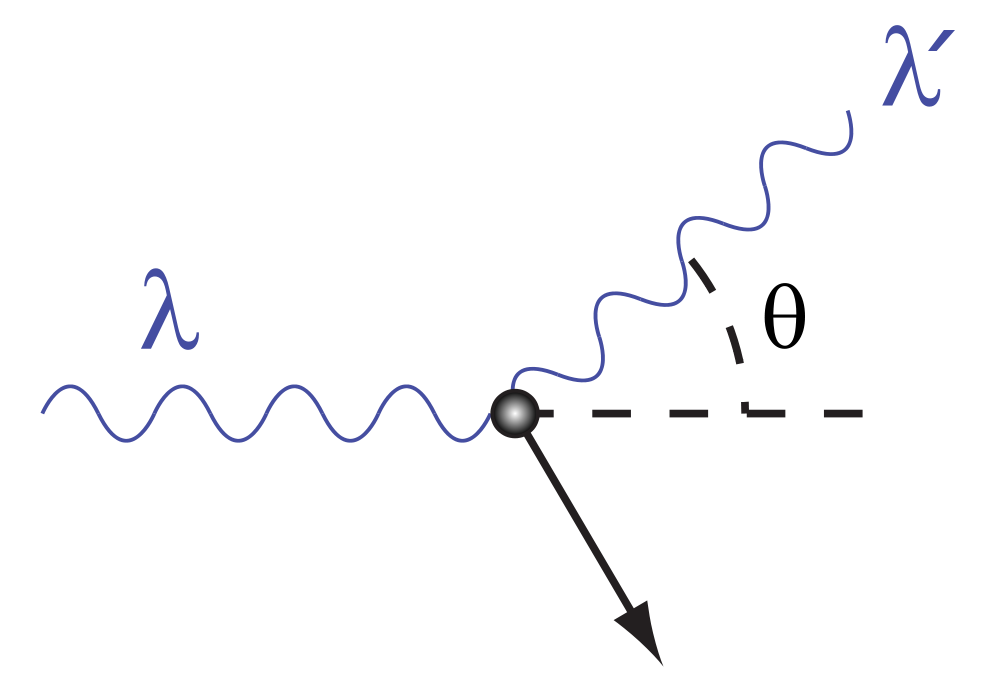
\includegraphics[width=0.45\textwidth]{ComptonScattering}
  \caption{Compton Scattering of a Photon off an Electron}
  \label{fig:ComptonScattering}
\end{figure}
\begin{align}
  \label{eqn:AFinalPhotonEnergy}
  \frac{1}{E'} -\frac{1}{E} = \frac{1}{m_e c^2}\left(1-\cos\theta\right) 
\end{align}
Using the conservation of energy, the energy given to the electron, $E_e$ must be equal to the difference in the initial and final photon energies \eqref{eqn:AEnergyElectron}
\begin{align}
  \label{eqn:AEnergyElectron}
  E_e &= E - E' \\ \notag
   &= E - \frac{E m_e c^2}{m_e c^2 + E (1-\cos\theta)}
\end{align}

\section{Differential Scattering Cross Section}
The probability of scattering and imparting energy is provided by the Klein-Nishina formula \eqref{eqn:AKleinNishina}.
\begin{align}
  \label{eqn:AKleinNishina}
  d\sigma = \frac{1}{2} r_0^2 \left(\frac{E'}{E}\right)^2 \left(\frac{E'}{E} + \frac{E}{E'}-\sin^2\theta\right)d\Omega
\end{align}
If $f(\theta)$ is defined as $f(\theta) = \frac{1}{2}\left(\frac{E'}{E}\right)^2 \left(\frac{E'}{E} + \frac{E}{E'}-\sin^2\theta\right)$ and assuming the scattering is isotropic leading to $d\Omega = \sin\theta d\theta d\phi$ it is then possible to express \eqref{eqn:AKleinNishina} as \eqref{eqn:AKleinNishinaShort}.
\begin{align}
  \label{eqn:AKleinNishinaShort}
    d\sigma = r_0^2 f(\theta)\sin\theta d\theta d\phi
\end{align}
It is then possible to integrate over $\phi$, and then divide by the differential scattering angle to arrive at \eqref{eqn:ADiffKleinNishina}.
\begin{align}
  \label{eqn:ADiffKleinNishina}
  d\sigma &=\int_{\phi=0}^{2\pi} r_0^2 f(\theta)\sin\theta d\theta d\phi\\
  \frac{d\sigma}{d\theta} &=2\pi r_0^2 f(\theta)\sin\theta
\end{align}
However the probability of scattering at a given kinetic energy of the electron is desired, $d\sigma/dE_e$.
With the chain rule and a few algebraic manipulations it is possible to arrive at \eqref{eqn:ADiffE}, and if the derivative of \eqref{eqn:AEnergyElectron} is taken with respect to $\theta$ the differential energy scattering can be expressed as \eqref{eqn:AdSdEKleinNishina}.
\begin{align}
  \label{eqn:ADiffE}
  \frac{d\sigma}{dE_e} & = \frac{d\sigma}{d\theta} \frac{d\theta}{dE_e} \\
   & = \frac{d\sigma}{d\theta} \left[\frac{dE_e}{d\theta}\right]^{-1} 
\end{align}
\begin{align}
  \label{eqn:AdSdEKleinNishina}
\frac{d\sigma}{dE_e} = 2\pi r_e^2 \sin \theta f(\theta)\left [ \frac{1+\frac{E}{m_e c^2}\left(1-\cos\theta \right)^2}{E^2 \sin \theta} \right ]
\end{align}

\section{Computational Spectra}
The probability of a Compton scattered electron having an energy $E$ was calculated by sampling (using a rejection method) for the scattering distribution derived in \autoref{eqn:AdSdEKleinNishina}.
This probability was then normalized into a probability density function and the cumulative density function was then calculated to yield the probability that an electron would be born at an energy.
% Something about the code is avialable . . .


    % MCNPX Model of the interaction rate
\chapter{MCNPX Tally Interactions}
The performance of films is simulated in MCNPX, a Monte Carlo transport code\cite{pelowitz_mcnpx_????}.

The interaction rate is calculated using the a cell flux tally in MCNPX and a tally multiplier card.
The tally multiplier card (FMn) is used to calculated any quantity of the form \eqref{eqn:FMCardForm} \cite{pelowitz_mcnpx_2006}
\begin{align}
  \label{eqn:FMCardForm}
  I &= C\int\phi(E)\Re_m(E)dE
\end{align}
where \definevar{$I$}{Interaction rate}, \definevar{$\phi(E)$}{Energy dependent fluence} , \definevar{$\Re_m(E)$}{Response function operator} and $C$ is an arbitrary scalar for normalization.
An general example of the use of the FM card is shown in Listing \ref{lst:GeneralFMExample}, which is taken from the MCNPX manual \cite{pelowitz_mcnpx_????}.
% See pg. 4-41 of the MCNP manual
\begin{lstlisting}[caption={[Example usage of the FM card]Example usage of the FM card to calculate the number of reactions per \si{\cm\cubed} of type R in cell 8 of material M. The normalization is by atomic density, signified by the -1},label={lst:GeneralFMExample}]
F104: N 8
FM104 -1 M R
\end{lstlisting}

The reaction rate $\iso[6]{Li}\left(\text{n},\text{t}\right)\alpha$ can be calculated by then applying the appropriate input for the FMn card and using an F4 card to calculate $\phi(E)$.
It should be noted that depending on the form of the cell flux card it may be necessary to normalize by the volume of the cell, $\forall$.
\nomenclature{$\forall$}{Volume of the cell}

This is shown in Listing \ref{lst:InteractionRateRPM}, where the reaction number is 105 and the material number of the detector is 3.
The interaction rate in a simulated RPM8 replacement detector is calculated in a similar manner as the simulation of the measured detectors; the interaction rate as computed by the \verb+FMn+ is multiplied by the source strength and volume if necessary.
An example of the MCNPX input cards is shown in Listing \ref{lst:InteractionRateRPM}.
Given that there the thermal response is not desired, there is no need to subtract out the differences between the spectra, and the interaction rate is simply \eqref{eqn:RPM8InteractionRate}.
Note that in this calculation the source strength is set to be \SI{1}{\nano\gram} \iso[252]{Cf}, which has a neutron emission rate of \SI{2.3E3}{neutron\per\second}.
This is in accordance with the direct evaluation of the PNNL criteria, which require a absolute neutron count rate of \SI{2.5}{count\per\second\per\nano\gram\iso[252]{Cf}}.
\begin{lstlisting}[caption={[RPM8 ${}^{6}\text{Li}\left(\text{n},\text{t}\right)\alpha$ Reaction Rate]RPM8 ${}^{6}\text{Li}\left(\text{n},\text{t}\right)\alpha$ Reaction Rate. The detector is all of the layers of cell 500 inside universe 610. This tally is multiplied by an SD card to normalize by the volume},label={lst:InteractionRateRPM}]
FC4 (n,t) Reactions in Thin Film (Neutron Detector)
F4:n (500<610)
SD4 1
FM4 -1 3 105
\end{lstlisting}
\begin{align}
  \label{eqn:RPM8InteractionRate}
  I_{\text{sim}} &= S_0 I \\
  &= \SI{2.3E3}{neutron\per\second} I
\end{align}

$I_{\text{sim}}$ provides the total number of simulated neutron interactions in the detector.

\section{Example of Layered Detector Geometry}
The following tables provide examples of the positions of the layered geometry used for the genetic algorithm. 
These geometries correspond to \autoref{fig:RPMLayeredRendering25} and \autoref{fig:RPMLayeredRendering5}, and \autoref{fig:RPMLayeredRendering75}.
% Optimal geometry tables.  All are PS Films
\begin{table}
	\caption[Optimal Layered Film Geometry for 7.5 interaction per second per nanogram Cf-252]{Optimal layered film geometry for an interaction rate of 7.5 interactions per second per nano-gram \iso[252]{Cf} in a 10\% \iso[6]{Li} loaded PS film. The positions shown in the table are the right boundary, where the detector starts at \SI{0.0}{\cm}. The genome representing this geoemtry is \texttt{01111101110100001000}.}
	\begin{tabular}{m{3cm} m{4cm}}
	\toprule
	Edge Position (\si{\cm}) & Material \\
	\midrule
0.635&Moderator\\
0.645&Detector\\
1.270&LightGuide\\
1.280&Detector\\
1.905&LightGuide\\
1.915&Detector\\
2.540&LightGuide\\
2.550&Detector\\
3.175&LightGuide\\
3.185&Detector\\
3.810&LightGuide\\
4.445&Moderator\\
4.455&Detector\\
5.080&LightGuide\\
5.090&Detector\\
5.715&LightGuide\\
5.725&Detector\\
6.350&LightGuide\\
6.985&Moderator\\
6.995&Detector\\
7.620&LightGuide\\
8.255&Moderator\\
8.890&Moderator\\
9.525&Moderator\\
10.160&Moderator\\
10.170&Detector\\
10.795&LightGuide\\
11.430&Moderator\\
12.065&Moderator\\
12.700&Moderator\\
	\bottomrule
	\end{tabular}
\end{table}
\begin{table}
	\caption[Optimal Layered Film Geometry for 5.0 interaction per second per nanogram Cf-252]{Optimal layered film geometry for an interaction rate of 5.0 interactions per second per nano-gram \iso[252]{Cf}  in a 10\% \iso[6]{Li} loaded PS film. The positions shown in the table are the right boundary, where the detector starts at \SI{0.0}{\cm}. The genome representing this geoemtry is \texttt{011101001000000}.}
	\begin{tabular}{m{3cm} m{4cm}}
	\toprule
	Edge Position (\si{\cm}) & Material \\
	\midrule
0.847&Moderator\\
0.857&Detector\\
1.693&LightGuide\\
1.703&Detector\\
2.540&LightGuide\\
2.550&Detector\\
3.387&LightGuide\\
4.233&Moderator\\
4.243&Detector\\
5.080&LightGuide\\
5.927&Moderator\\
6.773&Moderator\\
6.783&Detector\\
7.620&LightGuide\\
8.467&Moderator\\
9.313&Moderator\\
10.160&Moderator\\
11.007&Moderator\\
11.853&Moderator\\
12.700&Moderator\\
	\bottomrule
	\end{tabular}
\end{table}
\begin{table}
	\caption[Optimal Layered Film Geometry for 2.5 interaction per second per nanogram Cf-252]{Optimal layered film geometry for an interaction rate of 2.5 interactions per second per nano-gram \iso[252]{Cf} in a 10\% \iso[6]{Li} loaded PS film. The positions shown in the table are the right boundary, where the detector starts at \SI{0.0}{\cm}. The genome representing this geoemtry is \texttt{0011010000}.}
	\begin{tabular}{m{3cm} m{4cm}}
	\toprule
	Edge Position (\si{\cm}) & Material \\
	\midrule
1.270&Moderator\\
2.540&Moderator\\
2.550&Detector\\
3.810&LightGuide\\
3.820&Detector\\
5.080&LightGuide\\
6.350&Moderator\\
6.360&Detector\\
7.620&LightGuide\\
8.890&Moderator\\
10.160&Moderator\\
11.430&Moderator\\
12.700&Moderator\\
	\bottomrule
	\end{tabular}
\end{table}

    \chapter{Detector Characterization}
\label{chap:DetChar}
Repeated characterization techniques of the detector materials are necessary to ensure a fair comparison between different detector materials.
As the focus of this work was on effective scintillators the characterizations were designed to measure scintillation properties; namely the light yield of the detector and the count rate when exposed to different radiation sources.

\begin{itemize}
  \item Total Neutron Counts – provides a measure of how responsive the detector is to neutrons
  \item  Total Neutron Count Rate Per mg Absorber – provides a measure of how well the fabricated detector utilizes the neutron absorber in it. Indirectly this can be a measure of the amount of absorber in the detector
  \item  Gamma LLD – The position (in channel number) of where an LLD would have to be set in order to meet the criteria of \si{1E-6}
  \item  Fraction of Total Neutron Count Rate Above the Gamma LLD – this is a measure of how effective the film would be with an LLD set in order to meet the This is calculated by summing the counts above the gamma LLD and dividing by the total counts.
  \item  Alpha Peak – provides a clear indication of the light yield of the film from an alpha particle, which is one of the reaction products of the 6Li neutron interaction. The alpha peak is visible in thin films when other features may be lost (due to the range of the secondary electrons exceeding the thickness of the detector) because the range of the alpha is on the order of 30 microns.
  \item  Beta Average – characterizes the response of the film to electrons, account for the possibility that a film may not have a clearly defined feature due to energy escaping. Electrons are generated in the film from scattering events of photon interactions.
  \item  Alpha / Beta – characterizes the relative light yield of the detector from heavy charged particles to electrons.
  \item  Pulse Height Deficit – a measure the apparent energy loss (as seen from the pulse height) of a heavy charged ion compared to an electron. This is measured as the difference between the energy of the heavy ion and its apparent energy from the pulse height. It should be noted that this term closely resembles the phenomena described by pulse height defect as seen in semiconductors.
  \item  Photons per Neutron – a measure of the light yield of the film, or how many photons are produced per energy absorbed.
\end{itemize}

\subsection{Characterization Electronics and Sources}
Solid samples are characterized by mounting them with a thin layer of silicone optical grease (BC-630, index of refraction 2.465) onto a Philips XP2202B 10 Stage PMT most sensitive in the \SI{350}{\nm} to \SI{500}{\nm} region.
The PMT is then connected to a Canberra 2007P base, which also functions as a preamplifier.
The Canberra 2007P feeds into an Ortec 572A amplifier, and the amplified signal is inputted to an Ortec 926 MCB-ADC.
MAESTRO-32 is the used to read the signals from the MCB.
\autoref{fig:ElectronicsSetup} provides an overview of this setup.
\begin{figure}
  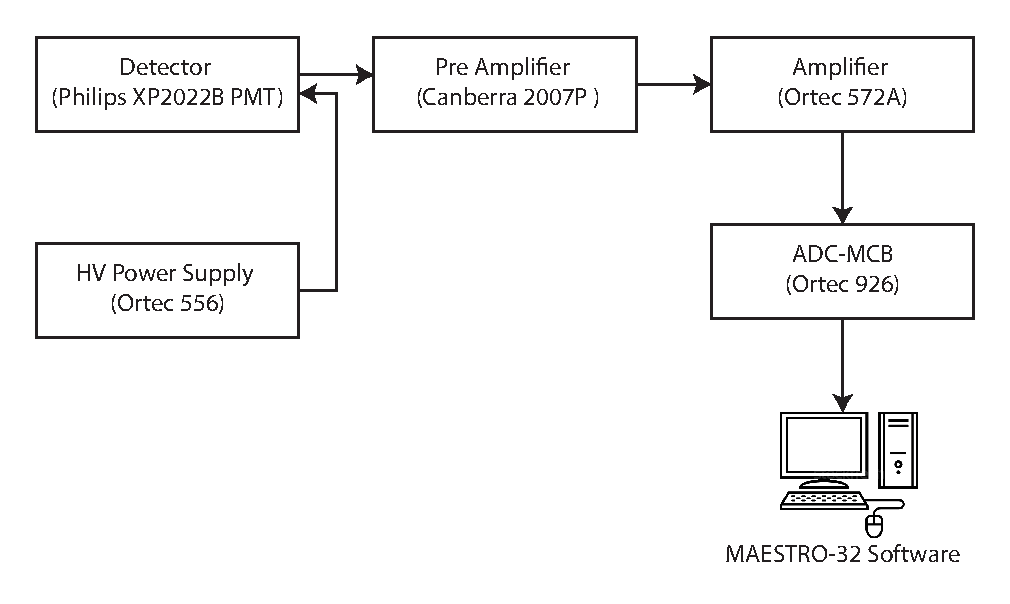
\includegraphics[width=0.5\textwidth]{ElectronicsSpectra}
  \caption[Optical Characterization Experiment Setup]{Electronic figure for measuring the spectra of materials in response to various radiation sources.}
  \label{fig:ElectronicsSetup}
\end{figure}
A general protocol has been developed in order to ensure that the measurements are made in a repeatable manner and verified with a reference.
\begin{enumerate}
  \item Verify that the instrumentation gains are stable by confirming that the reference neutron peak is in the same channel as for previous measurements. This is completed by setting the voltage and coarse gain to previously determined values, and then adjusting the fine gain until the peak of the lead spectra measurement occurs in the specified location,
  \item obtain a spectrum from an Am-241 alpha source,
  \item obtain a spectrum from a Cl-36 beta source,
  \item obtain a neutron spectrum from the Pb-shielded tube neutron irradiator,
  \item obtain a neutron spectrum from the Cd-shielded tube in the neutron irradiator,
  \item obtain a gamma spectrum in the gamma irradiator.
\end{enumerate}

\subsubsection{Neutron and Gamma Irridiators}
The neutron irradiator is a custom built \SI{0.59}{\ug} \iso[252]{Cf} source encased in 2” blocks of high density polyethylene (HDPE). 
The HDPE box is approximately 20” long, 12” wide, and 14” tall (\autoref{fig:NeutronIrridiator}). 
There are two detector 1/16” thick acrylic detectors wells, one surrounded by a 1/16” cadmium to shield out thermal neutrons, and the other surrounded by 1/16” of lead to shield out a similar amount of gammas as the cadmium well.
The \iso[252]{Cf} source is surrounded by stainless steel, which in turn is contained within a 2” diameter, 1/2” thick, 5 and 1/4” tall lead vessel.
\begin{figure}
  \centering
  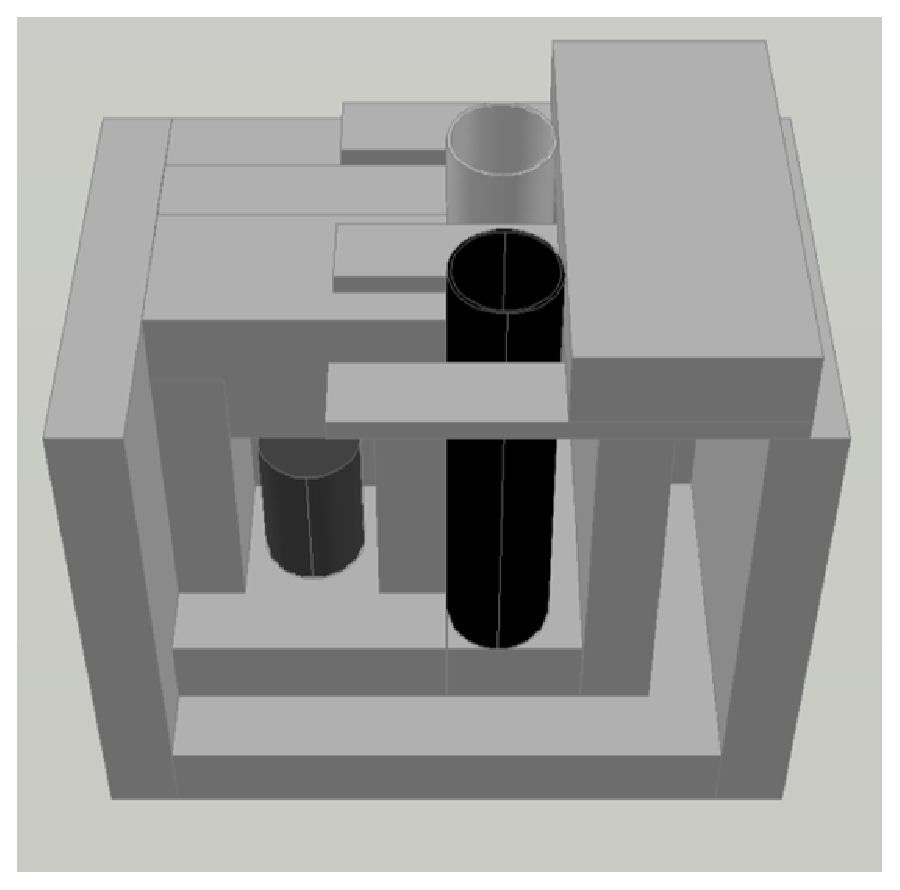
\includegraphics[width=0.5\textwidth]{NeutronIrridiator_CAD}
  \caption[CAD Rendering of Neutron Irridiator]{Schematic of the neturon irridiator.}
  \label{fig:NeutronIrridiator}
\end{figure}
The gamma sources consist of button sources (\iso[137]{Cs} up to \SI{10}{\u Ci} and \iso[60]{CO} up to \SI{1}{\u Ci}) as well as a gamma irradiator that produces a 10 mR/hr gamma field across the detector face. 
The irradiator consist of four 4”x8”x 2” lead bricks on the bottom with and additional four 4”x4”x2” lead bricks encased in an 1/8” metal box. 
The top four inches is HDPE. 
The overall dimensions of the detector are 14” by 12” by 12”. 

\section{Light Yeild}
The light yield of a spectrum describes how many photons are generated (and subsequently detected on a PMT) for a given material for a scintillation event from a radiation source.
In general, a feature, such as the Compton edge or neutron peak,  provides a unambiguous measure of light yield of a film. 
However, the thinner films do not always have such a clearly defined feature, and thus an alternative measure needs to be formulated.
The spectral average is then defined as \eqref{eqn:spectralAverage} where $p(x)$ is the measured spectrum as a function of channel number $x$ which describes the count rate average channel number, normalized by the total count rate.
\begin{align}
	<\mu> = \frac{\int_0^\infty x p(x) dx}{\int_0^\infty p(x) dx}
	\label{eqn:spectralAverage}
\end{align}
The limits of integration in \eqref{eqn:spectralAverage} are from the lowest to the highest channel number.
While the spectral average does provide a clear representation of a spectra, it fails to capture the shape of the spectra and tends to underestimate the spectra, as most spectra a skewed having the majority of their counts in the low channel region.

The light yield of fabricated samples that were characterized was completed by comparing the spectrum average of a sample to that a sample of a known light yield.
This is shown for neutrons in \eqref{eqn:neutronLY}, and for gammas in \eqref{eqn:gammaLY}.
GS20 is normally used as the reference sample, having a reported light yield of \SI{3,800}{photons \per\MeV} and \SI{6,200}{photons \per neutron} \cite{carel_w.e_inorganic-scintillator_2001,knoll_radiation_2009}.
\begin{align}
	LY_{n,\text{sample}} &= LY_{n,\text{ref}} \left( \frac{<n>_\text{sample}}{<n>_\text{ref} } \right )\\
	&= \SI{6,200}{photons\per neutron} \left( \frac{<n>_\text{sample}}{<n>_\text{ref} } \right )
	\label{eqn:neutronLY}
\end{align}
\begin{align}
	LY_{\gamma,\text{sample}} &= LY_{\gamma,\text{ref}} \left( \frac{<\gamma>_\text{sample}}{<\gamma>_\text{ref} } \right )\\
	&= \SI{3,800}{photons\per\MeV} \left( \frac{<\gamma>_\text{sample}}{<\gamma>_\text{ref} } \right )
	\label{eqn:gammaLY}
\end{align}

\section{Intrisinic Efficiency}
\label{sec:IntEff}

Often times it is necessary to relate the performance of a detector to number of particles that cross the detector, this is completed using the intrinsic efficiency.
Thus the intrinsic efficiency it is a measure at how efficient the detector is at detecting radiation, normalized to the amount of radiation that crosses the detector.
The intrinsic efficiency is defined as the ratio between the counts recorded in the detector and the number of impingement radiation on the detector\cite{knoll_radiation_2009}, expressed as \eqref{eqn:intEffDef},
\begin{align}
  \label{eqn:intEffDef}
  \epsilon_{int} = \frac{N_c}{N_i}
\end{align}
where:
\begin{itemize}
  \item[] \definevar{$\epsilon_{int}$}{intrinsic efficiency},
  \item[] \definevar{$N_c$}{number of counts recorded by the detector}, and
  \item[] \definevar{$N_i$}{quanta of radiation incident upon the detector}.
\end{itemize}
In order to determine the intrinsic efficiency of a detector it is then necessary to determine the performance of the detector (easily completed by measuring the detector) and the number of radiation impingement upon the detector (usually accomplished through calculation on simulation).

The quanta of radiation incident upon the detector can be expressed as the product of two components: the source strength and the solid angle, \eqref{eqn:QuantaIncidentDef},
\begin{align}
  \label{eqn:QuantaIncidentDef}
  N_i = \Omega S_0
\end{align}
where:
\begin{itemize}
  \item[] \definevar{$S$}{source strength}, and 
  \item[] \definevar{$\Omega$}{fraction of solid angle detector subtends}.
\end{itemize}
Radiation sources generally decay from their initial source strength according to the half-life of the source.
The time dependent source strength, $S(t)$ can then be expressed as \eqref{eqn:HalfLife}, where \definevar{$S_0$}{initial source strength}, \definevar{$t_{1/2}$}{half life} and \definevar{$t$}{age of source}.
\begin{align}
  \label{eqn:HalfLife}
  S(t) = S_0 e^{-\frac{\ln{2}}{t_{1/2}} t}
\end{align}

The fraction of the source solid angle the detector subtends, $\Omega$, is computed using MCNPX. 
A F1 tally, defined in \eqref{eqn:F1Def}, is employed over the detector surface with two cosine bins, $-1<\cos\theta<0$ and $0<\cos\theta<1$, which divide the tally into particles that enter the surface and particles that leave the surface, respectively.
\begin{align}
  \label{eqn:F1Def}
  F1 &= \int_A dA \int_E dE \int_{4\pi} d\Omega ;;\vec{n}\cdot\vec{J}(\vec{r},E,\vec{\Omega}) \\
 %  &= \int_A dA \int_E dE \int_{4\pi} d\Omega \vec{n}\cdot\vec{\Omega}\Phi(\vec{r},E,\vec{\Omega}) \notag
\end{align}
In \eqref{eqn:F1Def} the position $\vec{r}$\nom{$\vec{r}$}{position}, direction $\vec{\Omega}$\nom{$\vec{\Omega}$}{direction} and energy $E$ \nom{$E$}{energy} dependent particle current $\vec{J}$ \nom{$\vec{J}$}{particle current} is integrated over the entire area, energy and direction normal to the surface of the area.
As macro-bodies are used for the surfaces of the detector, $-1<\cos\theta<0$ represents the particles that cross into the surface and $0<\cos\theta<1$ the particles that leave the surface.
In the case where macrobodies are not used to create the cell, the reader is referred to the MCNPX manual for more details.

The count rate of a detector is found by integrating the measured spectra, $p(x)$, over some bounds of integration.
It is then possible to express the intrinsic efficiency as a function of a mathematical lower level discriminator (MLLD) of the measured spectra \footnote{The MLLD behaves essentially as a physical lower level discriminator in that all counts below this value are discarded.} in order to determine at what MLLD the intrinsic efficiency is less then a value.
Equation \eqref{eqn:MLLDDef} shows such a formulation of the intrinsic efficiency as a function of a MLLD, where the upper bond is assumed to be the end of the spectra or highest recorded channel of the analog to digital converter.
\begin{align}
	\label{eqn:MLLDDef}
	\epsilon_{int}(MLLD) &= \frac{\int_{MLLD}^\infty p(x)dx}{N_i}
\end{align}

\subsection{Neutron Intrinsic Efficiency}
The number of counts upon a detector is measured by irradiating the detector in a lead and cadmium well of the neutron irridiator to determine $N_i$, and then simulating that geometry in bench-marked MCNPX in order to determine the number of neutrons incident on the detector\footnote{MCNPX simulations were benched-marked against GS20 and against polymer films, having 4\% and 15\% agreement to measured count rate, respectively.}.
The determination of $N_i$ consists of two parts: 1) determining the number of neutrons crossing the detector surface in the lead and cadmium wells and, 2) determining the source strength.
The \iso[252]{Cf} source was \SI{0.59}{\ug} on July 2, 2009.
Given that the half-life of \iso[252]{Cf} is 2.64 years and \iso[252]{Cf} has a spontaneous neutron emission rate of \SI{2.3E6}{neutron\per\second\per\micro\gram} the time dependent source strength can be calculated as \eqref{eqn:Cf252SourceStrength}.
\begin{align}
  \label{eqn:Cf252SourceStrength}
  S(t) &= S_0 e^{-\frac{\ln{2}}{t_{1/2}} t} \\ \notag 
    &= \SI{0.59}{\ug} \iso[252]{Cf} \;\frac{\SI{2.3E6}{neutron\per\second}}{\si{\ug} \iso[252]{Cf}}\; e^{-\frac{ \ln{2}}{\SI{2.64}{year}}t}  \\ \notag
    &= \SI{1.357E6}{neutron\per\second}\; e^{-\frac{ \ln{2}}{\SI{2.64}{year}}t} 
\end{align}

Table \ref{tab:NeutronSolidAngle} summarizes the incident flux for a number of different detector sizes and heights.
The fraction of solid angle subtended by other geometries can be computed by interpolation on the values of this table, as shown in the examples calculations.
It should be noted that there is considerable variation in the neutron flux in the detector wells, as shown in Figure \ref{fig:NeutronFluxProfiles}.
Thus, even though the calculations are accurate to less than a percent, the physical error on the intrinsic efficiency will be much higher due to uncertainty in where the detector was placed in the well.

\begin{table}
	\centering
	\caption[Simulated Thermal Neutron Solid Angle for Various Film Radii]{Simulated Neutron Solid Angle for Various Film Radii in the net spectra. The film radii are shown in seperate columns, with the thickness in rows. The thermal spectra (shown) is the subtraction of the lead and cadmium wells.}
	\label{tab:NeutronSolidAngle}
	\begin{tabular}{c | c c c c c c}
Thickness (\si{\cm})	&	\SI{1}{\cm}	&	\SI{1.27}{\cm}	&	\SI{1.905}{\cm}	&	\SI{2}{\cm}	&	\SI{2.5}{\cm}	&	\SI{2.54}{\cm} \\ \hline
0.0025	&	0.00055	&	0.00089	&	0.00204	&	0.00225	&	0.00351	&	0.00362	\\
0.005	&	0.00055	&	0.00090	&	0.00204	&	0.00224	&	0.00350	&	0.00361	\\
0.01	&	0.00055	&	0.00089	&	0.00204	&	0.00223	&	0.00348	&	0.00359	\\
0.015	&	0.00055	&	0.00089	&	0.00202	&	0.00222	&	0.00346	&	0.00357	\\
0.03	&	0.00056	&	0.00090	&	0.00201	&	0.00221	&	0.00341	&	0.00353	\\
0.1	&	0.00058	&	0.00093	&	0.00202	&	0.00220	&	0.00334	&	0.00347	\\
0.2	&	0.00063	&	0.00099	&	0.00208	&	0.00225	&	0.00338	&	0.00349	\\
0.5	&	0.00080	&	0.00119	&	0.00234	&	0.00251	&	0.00365	&	0.00375	\\
1	&	0.00109	&	0.00159	&	0.00286	&	0.00306	&	0.00427	&	0.00437	\\
2	&	0.00170	&	0.00233	&	0.00389	&	0.00412	&	0.00544	&	0.00555	\\
	\end{tabular}
\end{table}
\begin{figure}
	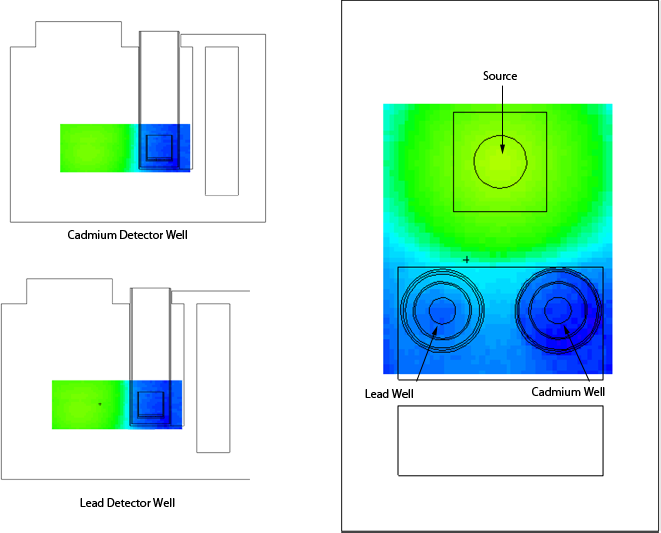
\includegraphics[width=\textwidth]{SpatialNeutronFlux}
  \caption[Neutron Flux Profiles of the Lead and Cadmium Wells]{Neutron Flux Profiles of the Lead and Cadmium Wells. Lighter colors correspond to a higher neutron population. The effect of the cadmium shielding is observed in the depression of the flux in the lower right by the cadmium well.}
  \label{fig:NeutronFluxProfiles}
\end{figure}

\subsection{Gamma Intrinsic Efficiency}
The gamma irridiator consists of a \SI{97}{\micro Ci} \iso[60]{Co} (January 1st, 2012) inside of a steel pipe encased in lead bricks.
The gamma intrinsic efficiency is calculated by simulating the fraction of solid angle the detector subtends and then using radioactive decay to model the \iso[60]{Co} source.
The \iso[60]{Co} source strength is calculated according to \eqref{eqn:Co60SourceStrength}. 
As there are two photons emitted from each \iso[60]{60} decay, in order to normalize the MCNPX source strength it is necessary to multiply the single photon activity by two.
Tabulated solid angle fractions are in Table \ref{tab:GammaSolidAngle}, and once again interpolation can be used for geometries not enumerated.
These values were extracted from an MCNPX simulation using an F1 tally as described above.
\begin{align}
  \label{eqn:Co60SourceStrength}
  S &= S_0 e^{-\frac{\ln{2}}{t_{1/2}} t} \\ \notag 
    &= \SI{97}{\micro Ci} \iso[60]{Co}\; \frac{\SI{3.7E10}{decay\per\second}}{\si{Ci}} \;\frac{2\text{photon}}{decay}\;e^{-\frac{ \ln{2}}{\SI{5.27}{year}}t}  \\ \notag
    &= \SI{7.178E6}{photon\per\second}\;e^{-\frac{ \ln{2}}{\SI{5.27}{year}}t} 
\end{align}
\begin{table}
	\centering
	\caption{Simulated Gamma Solid Angle for Various Film Radii}
	\label{tab:GammaSolidAngle}
	\begin{tabular}{c | c c c c c c}
Thickness (\si{\cm})	&	\SI{1}{\cm}	&	\SI{1.27}{\cm}	&	\SI{1.905}{\cm}	&	\SI{2}{\cm}	&	\SI{2.5}{\cm}	&	\SI{2.54}{\cm} \\ \hline
0.0025	&	0.0060	&	0.0095	&	0.0206	&	0.0226	&	0.0347	&	0.0357\\
0.005	&	0.0060	&	0.0095	&	0.0206	&	0.0226	&	0.0347	&	0.0357\\
0.01	&	0.0060	&	0.0095	&	0.0206	&	0.0226	&	0.0347	&	0.0357\\
0.015	&	0.0060	&	0.0095	&	0.0206	&	0.0226	&	0.0347	&	0.0357\\
0.03	&	0.0060	&	0.0095	&	0.0206	&	0.0227	&	0.0347	&	0.0357\\
0.1	&	0.0060	&	0.0096	&	0.0207	&	0.0227	&	0.0348	&	0.0358\\
0.2	&	0.0061	&	0.0097	&	0.0209	&	0.0229	&	0.0349	&	0.0360\\
0.5	&	0.0063	&	0.0099	&	0.0212	&	0.0232	&	0.0353	&	0.0364\\
1	&	0.0066	&	0.0103	&	0.0217	&	0.0237	&	0.0359	&	0.0379\\
2	&	0.0071	&	0.0109	&	0.0225	&	0.0247	&	0.0371	&	0.0382\\
3	&	0.0075	&	0.0114	&	0.0233	&	0.0255	&	0.0381	&	0.0392\\
4	&	0.0079	&	0.0119	&	0.0240	&	0.0262	&	0.0390	&	0.0401\\
	\end{tabular}
\end{table}
It should be noted that the gamma irradiator detector well is encased in a 1/2 inch steel pipe which is surrounded by lead, providing a beam like geometry while also introducing lower energy photons. 
The contribution of these lower energy photons is shown in Figure \ref{fig:PhotonFluxAllEnergies}, and it is evident that these contributions are a magnitude less than the contributions from the primary photons of the \iso[60]{Co} decay.
\begin{figure}
  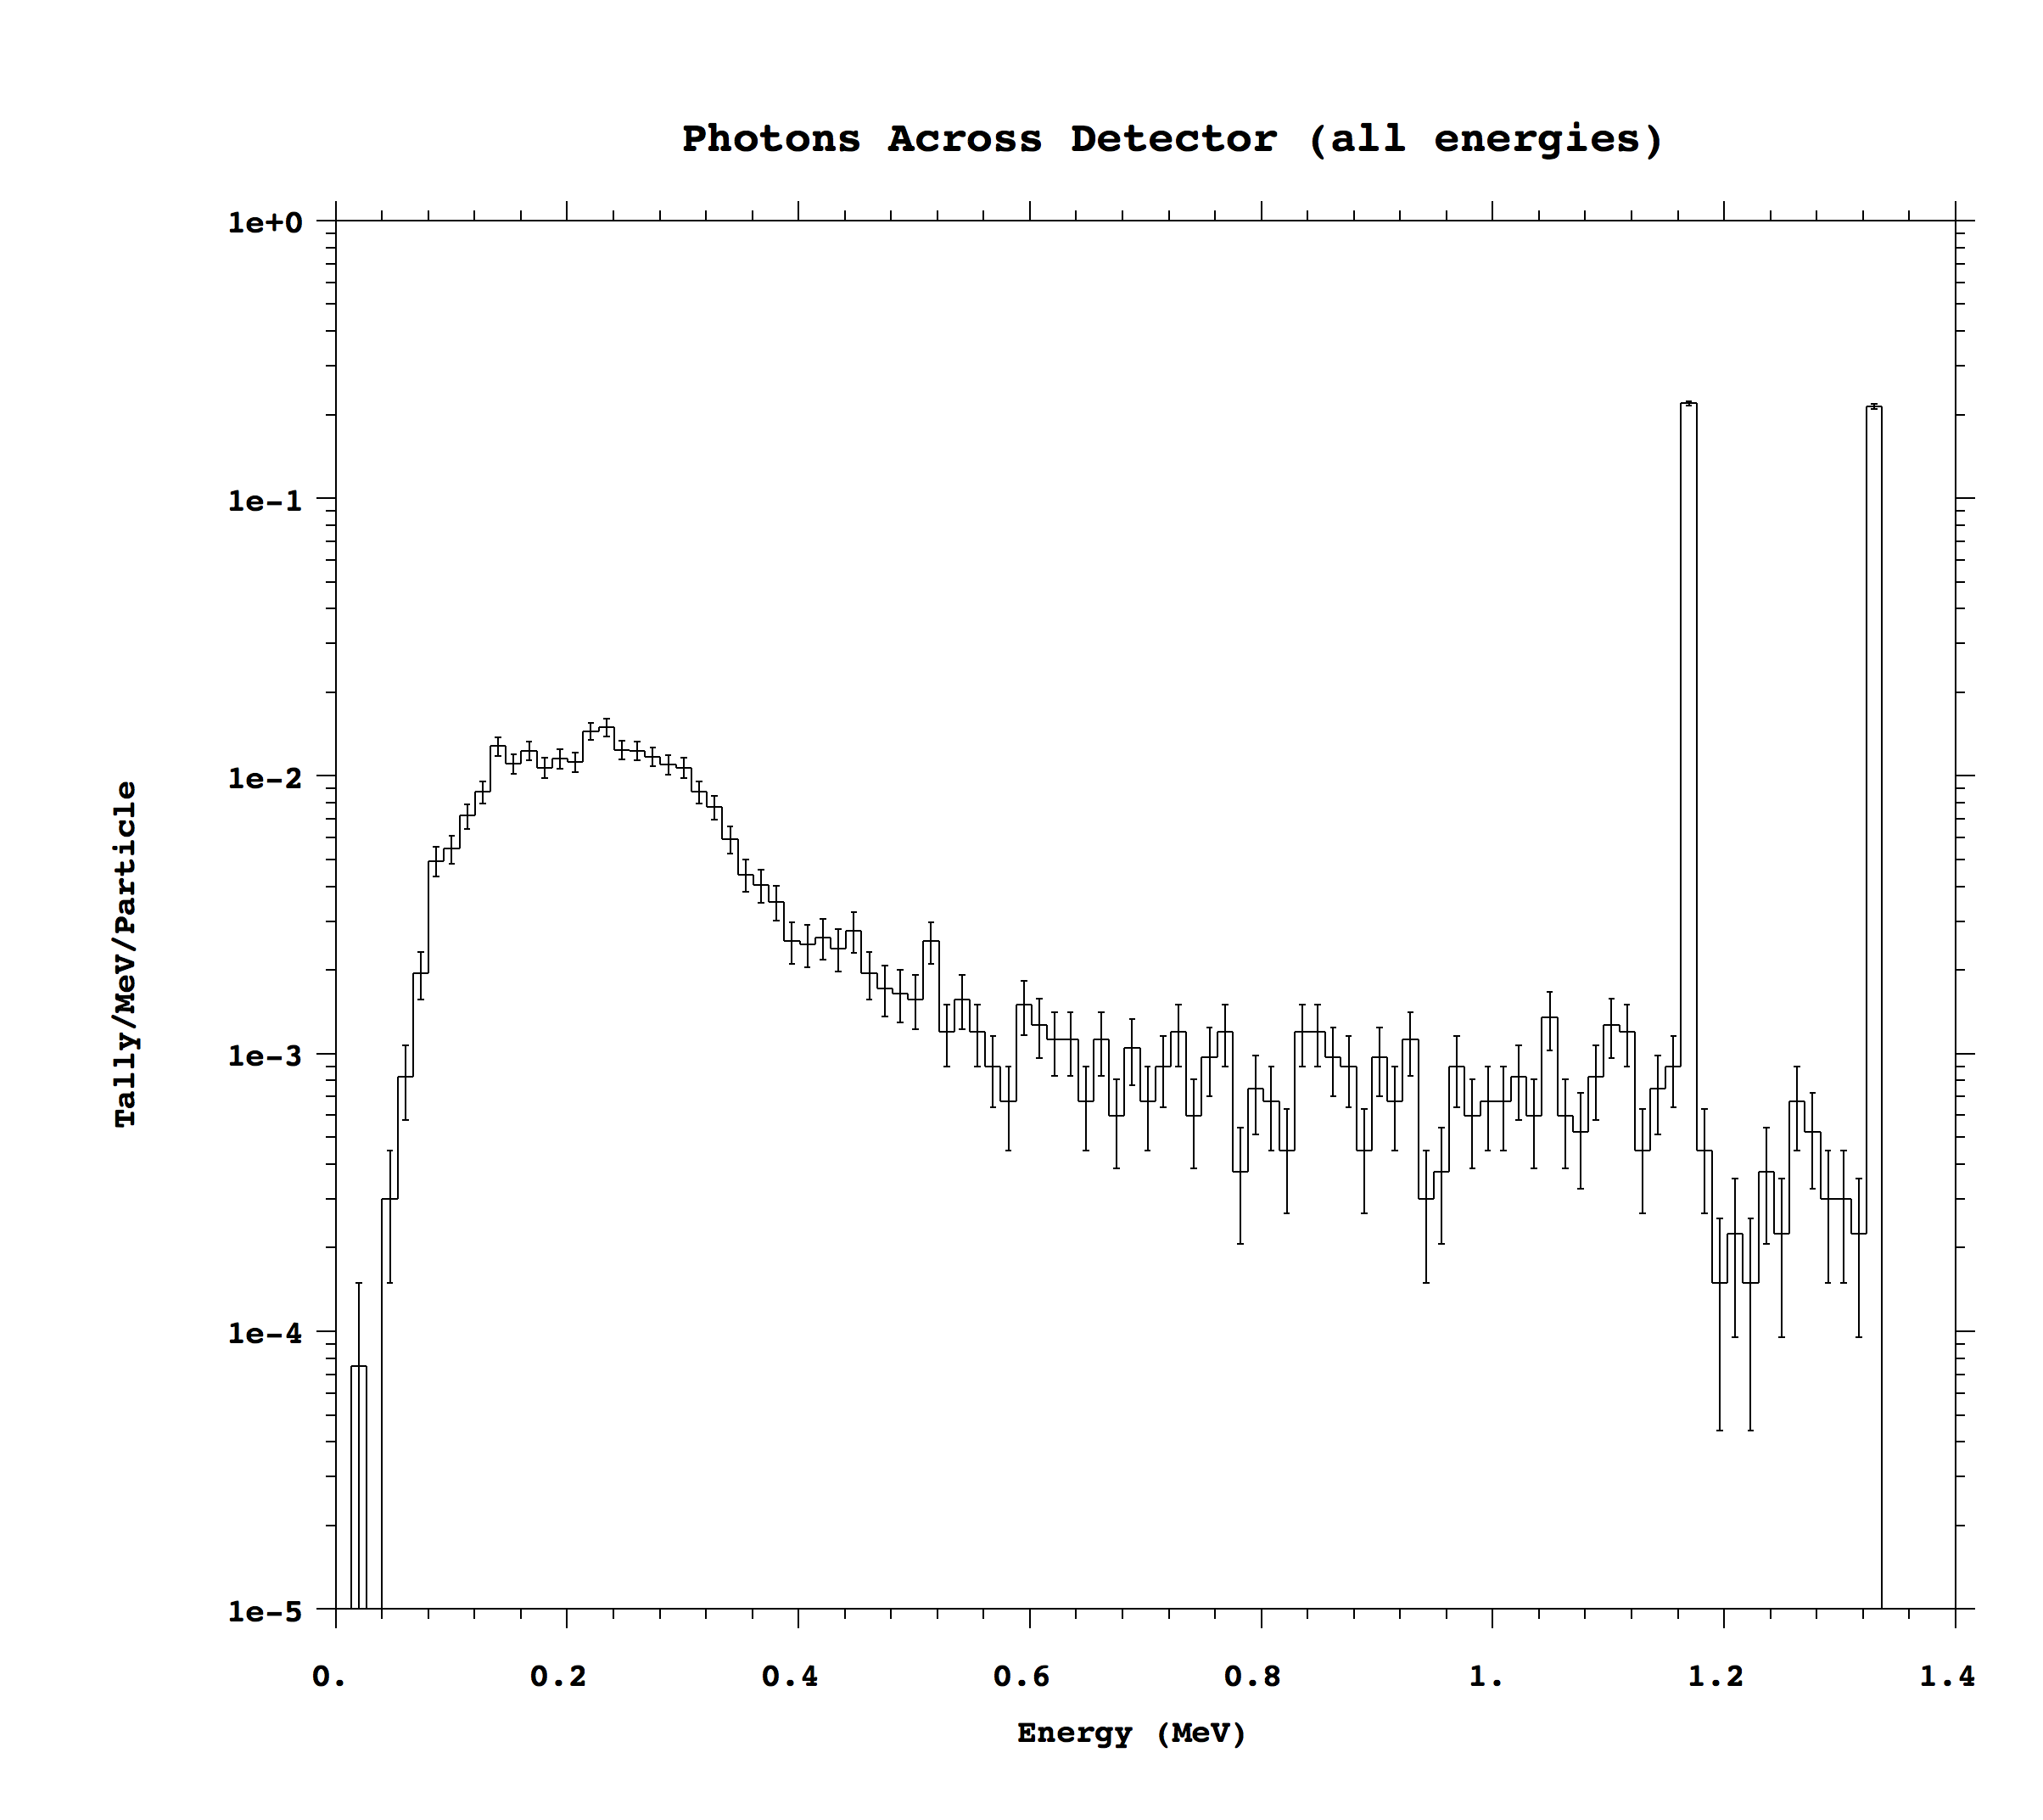
\includegraphics[width=\textwidth]{PhotonEnergyDist}
	\caption[Photons Incident upon Detector]{Photons incident upon a detector from an \iso[60]{Co} source.  The two \iso[60]{Co} photons (\SI{1.17}{\MeV} and \SI{1.33}{\MeV}) make up the majority of the incident photons.}
  \label{fig:PhotonFluxAllEnergies}
\end{figure}
Table \ref{tab:GammaSolidAngle} considers the contributions from all sides, but it is evident that the contributions from the side scattering is not large as 100 times increase in the thickness (\SI{50}{\um} to \SI{5}{\mm}) results in only a 4\% increase in the number of particles crossing the detector.


    %%%%%%%%%%%%%%%%%%%%%%%%%%%%%%%%%%%%%%%%%%%%%%%%%%%%%%%%%%%%%%%%%%%%%%%%%%%
%                                                                         %
%                              Start of Content                           %
%  This material was stolen from DetectorComparions located in:           %
% MillerResearch/documentation/ExperimentWriteUps                         %
%%%%%%%%%%%%%%%%%%%%%%%%%%%%%%%%%%%%%%%%%%%%%%%%%%%%%%%%%%%%%%%%%%%%%%%%%%%
\chapter{Measured Polymeric Film Detectors}
\label{chap:MeasuredFilmPerfomance}
\section{Introduction}

The potential application  of a material for use in a Radiation Portal Monitor (RPM) can be evaluated by measurements of the detector's sensitivity to gammas and the detector's response to neutrons.
A detector material might be a possible replacement if the there exists a neutron response that can be differentiated from photons for given sensitivity of gammas, namely \num{1E-6}.
A simple way to discriminate between gammas and neutrons is to use a pulse height discriminator, above which the detector detector will only record one photon out a million as a neutron.
Under this framework it is then possible to develop a mathematical lower level discriminator (MLLD) of the pulse height spectrum to function as this pulse height discriminator, and to then formulate the sensitivity requirement as the gamma intrinsic efficiency as a function of MLLD.
Six detectors (three boron loaded plastic scintillators, one LiF:ZnS(Ag) doped screen, GS20, a post processed composite PEN film, and a polystyrene) were then evaluated for their ability to perform in a RPM. 
The thickness of these detectors and mass of the absorber are shown in \autoref{tab:PhysicalProperties}.
\begin{table}
\centering
\caption[Detector Physical Characteristics]{Physical characteristics of the detector.}
\label{tab:PhysicalProperties}
  \begin{tabular}{p{6cm}| m{2cm} m{2cm} p{2.5cm}}
  \toprule
    & Absorber & Thickness &  Mass Absorber (mg) \\
    \midrule
    EJ 254 2.5\% & \iso[10]{B} & 1/4" & 59.5 \\
    EJ 254 1\% & \iso[10]{B} & 1/4" & 23.8 \\
    EJ 254 5\% & \iso[10]{B} & 3/4 & 356.1 \\
    EJ 425 HD2-PE & \iso[6]{Li} & \SI{0.1}{\mm} & 17.5 \\
    GS20 & \iso[6]{LI} & \SI{2}{\mm} & 155 \\
    Post Processed Composite PEN Film & \iso[6]{Li} & $\approx$ \SI{212}{\um} & 42.42 \\
    PS Film & \iso[6]{Li} & \SI{50}{\um} & 2.71 \\
    \bottomrule
  \end{tabular}
\end{table}

\section{Methods}
The neutron performance was determined by the \iso[252]{Cf} irridiator previously described, and the gamma source was the \iso[60]{Co} irridiator.
Due to the wide range of light output of these films it was necessary to use a two voltages (\SI{1000}{\volt} and \SI{1180}{\volt}) in order to capture the entire spectra on an ADC with a zero to \SI{10}{\volt} range with repeatable resolution.
However, a measurement of the GS20 peak in the lead well was always recorded which then allowed the spectra to be tied together based on this feature, as shown in \autoref{eqn:SettingScale}.
\begin{align}
  \label{eqn:SettingScale}
  \text{Feature at Setting A} &= \frac{\text{GS20 Peak at Setting A}}{\text{GS20 Peak at Setting B}} \;\; \left( \text{Feature at Setting B}\right)
\end{align}
The count rates are not scaled for gain and voltage settings as they should remain constant as long as counts are not pushed below the lower level discriminator or cause roll-off.
\subsection{Neutron Performance above Gamma Discriminator}
An accurate measure of the neutron performance above the pulse height discriminator is essential for the comparison between detector materials.
In \autoref{fig:GammaMLLDIntEff} it is shown that the location of the MLLD is a pretty stable measurement for PS films of a different thickness.
\begin{figure}
  \centering
  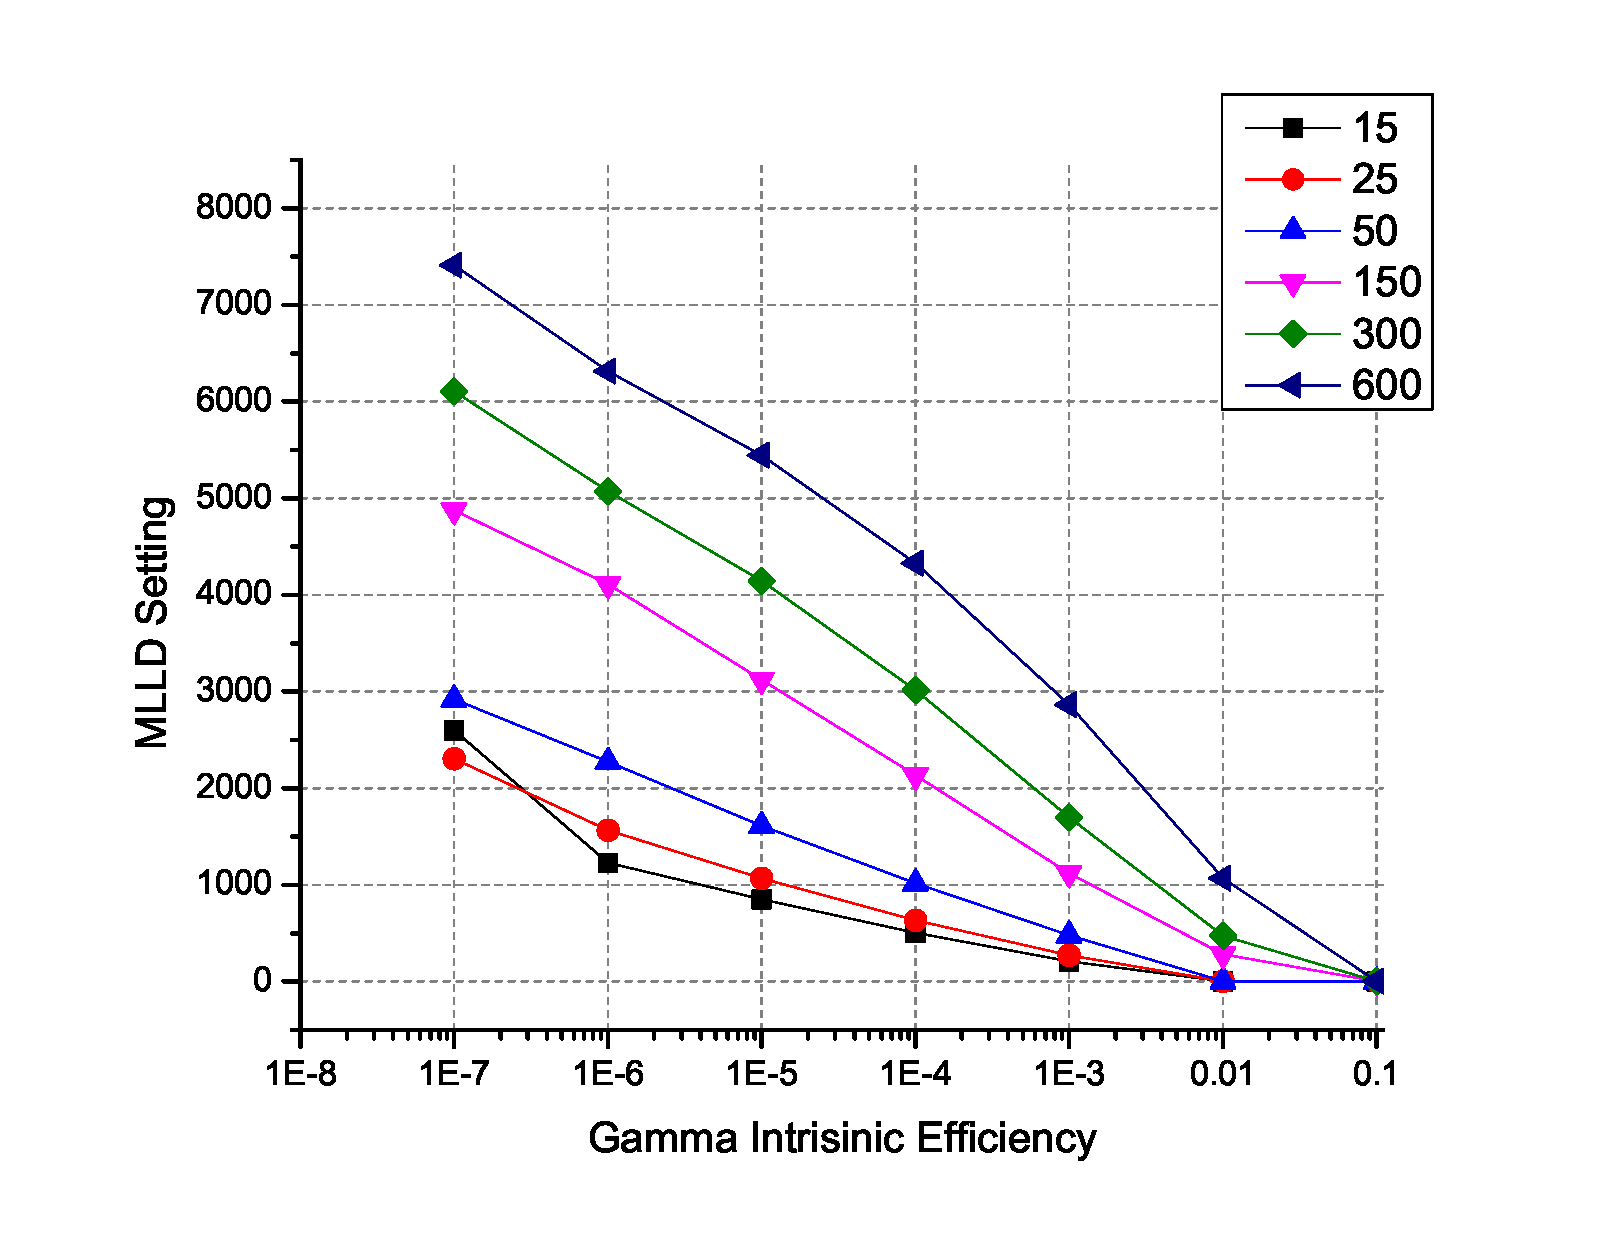
\includegraphics[width=\textwidth]{PS_IntEffMLLD_LiF}
  \caption[Stability of Lower Level Discriminator]{The mathematical lower level discriminator (MLLD) as a function of intrinsic effigies for 10\% PS films of various thickness. The linear nature suggest that the determination of the MLLD is repeatable.}
  \label{fig:GammaMLLDIntEff}
\end{figure}
However, in previous work which focused on using the fraction of neutron counts above the MLLD it was observed that the fraction (as it is normalized by the entire count rate) is very susceptible to sample to sample variations in the low energy channels.
Therefore, after extensive studies using the polystyrene matrix a more stable measure was found by simply integrating the counts in the neutron spectra above the MLLD and then normalizing by the mass of neutron absorber in the samples (\autoref{eqn:CountRateAbovePerMass}).
While this method does not have the errors associated with summing over the low channels, it does require an accurate measure of the mass of \iso[6]{Li} in the sample.
Alternative methods would also probably be stable, but they are not discussed here.
\begin{align}
\label{eqn:CountRateAbovePerMass}
\eta = \frac{\int_{\text{MLLD}}^\infty p(x)dx}{\text{Neutron Absorber Mass}}
\end{align}

\section{Results}
The following figures, \autoref{fig:Co60Spectra} and \autoref{fig:PbWellSpectra}, show the measured spectra of the detectors for neutrons and gammas.
It is clear that the EJ-254 (boron loaded plastic) detectors will have poor performance because of their large gamma response.
The EJ-426 (LiF:ZnS(Ag)) has the lowest response, and it is not clear if the tail of the spectra is due to actual counts or background.
In the neutron spectra it was decided to only plot the performance of the best EJ-254 (though \autoref{fig:EJ254Perf} display the performance of all EJ-254 films).
It is observed that the LiF:ZnS(Ag) is much brighter than the other films, and it is noted that the post processed composite PEN has a higher light output than the commercial EJ-254 (based on the peak location).
\begin{figure}
  \centering
  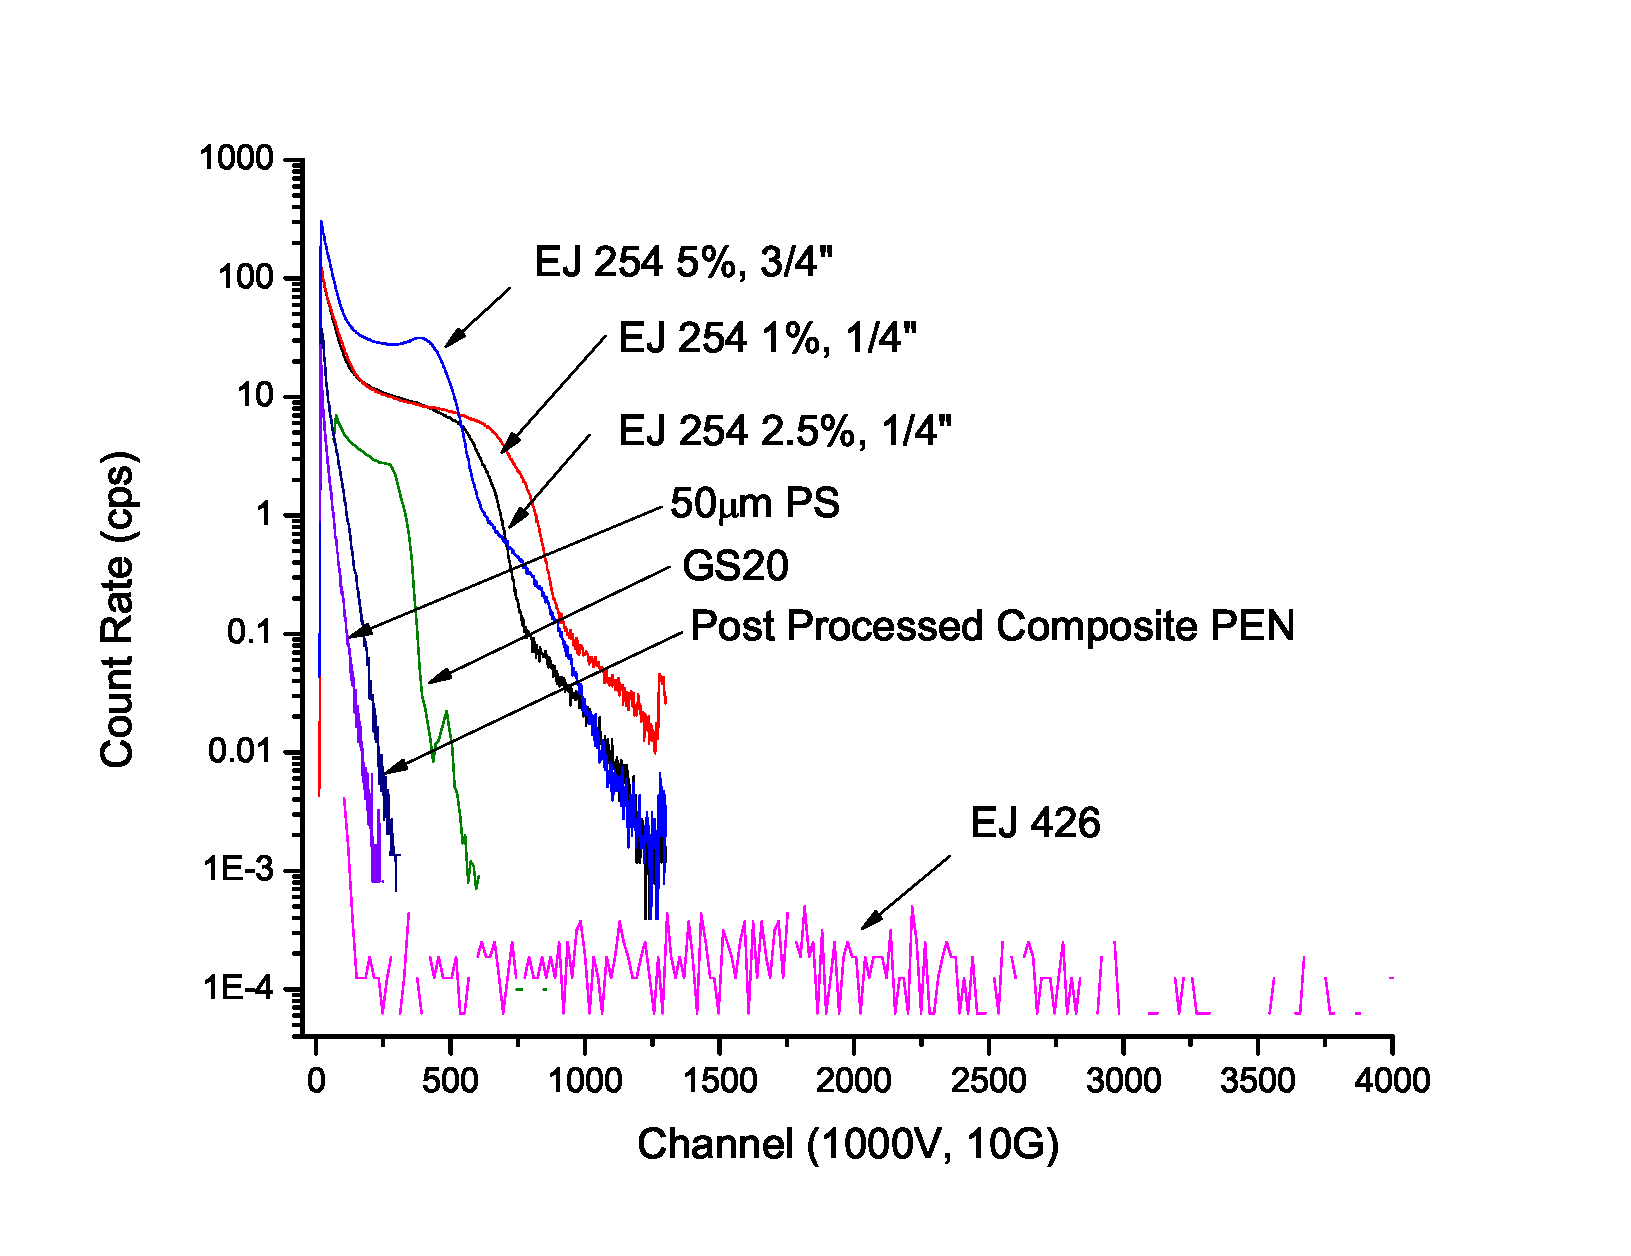
\includegraphics[width=\textwidth]{SampleComparions_Co60Spectra}
  \caption[Gamma Response of Measured Detectors]{Gamma Response from \iso[60]{Co} source of measured detectors.}
  \label{fig:Co60Spectra}
\end{figure}
\begin{figure}
  \centering
  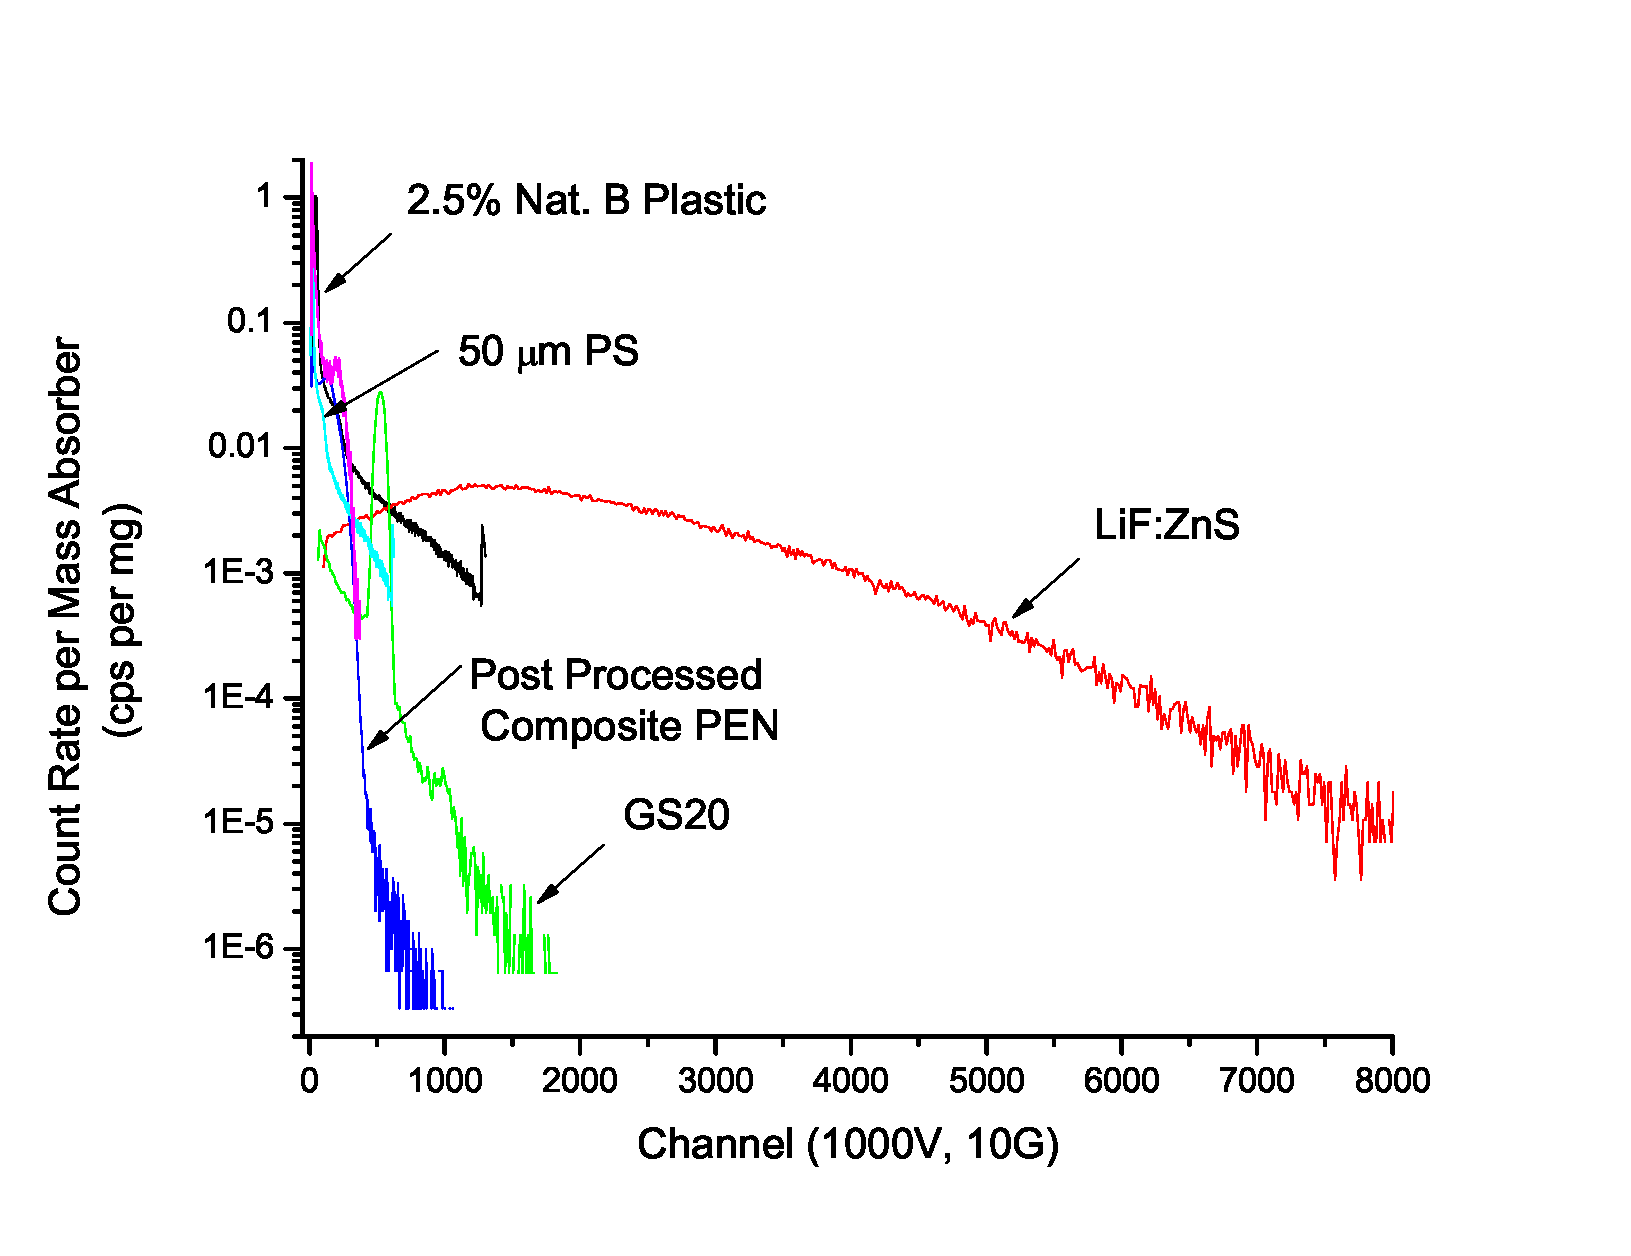
\includegraphics[width=\textwidth]{SampleComparison_PbCRperMg}
  \caption[Neutron Response of Measured Detectors]{Neutron Response (lead well) of the measured detectors. The count rate has been normalized by the mass of neutron absorber in the detector.}
  \label{fig:PbWellSpectra}
\end{figure}
The average channel number of the neutron and gamma spectra of each detector was calculated and are presented in \autoref{tab:AvgChNG}.
The average was computed for the neutrons in the thermal well to avoid the low energy channels from shifting the spectra away from any peak location.
It should be noted that for EJ-254 the low channel number average is correct; this feature was identified as the neutron peak.
Eljen publishes the light yield for the 1\% boron as 9,200 photons per MeVee, 8,600 photons per MeVee for the 2.5\% boron, and 7,500 photons per MeVee for the 5\% boron, and \autoref{tab:AvgChNG} shows agreement to these values.
C.W.E van Eijk has published the light yield of LiF:ZnS as 75,000 photons per MeVee, which is close to our measured value of 72,000 photons per MeVee.
\begin{table}
  \centering
  \caption[Average Channel Number of Gamma and Neutron Spectra]{Average channel number of gamma and the thermal neutron spectra.  The channel averages are scaled to 1,000V, 10G. The light yields are scaled to GS20 having 3,800 photons per MeV, and 6,250 photons per Neutron.}
  \label{tab:AvgChNG}
  \begin{tabular}{m{4cm}| m{2cm} m{2cm} |m{2cm} m{2cm}}
    \toprule
        &\multicolumn{2}{|c|}{Gamma}&\multicolumn{2}{|c}{Neutron}\\
        & Average Channel& Photons per MeVee & Average Neutron Channel & Photons per Neutron\\
    \midrule
    EJ 254 2.5\%, 1/4"&	183.41	&	8,100	&	54.06	&	640	\\
    EJ 254 1\%, 1/4"&	216.25	&	9,500	&	65.04	&	780	\\
    EJ 254 5\%, 3/4"&	176.49	&	7,800	&	39.56	&	479	\\
    EJ 426 HD2&	1636.53	&	72,000	&	2018.	& 	24,000	\\
    GS20 &	172.76	&	3800.00	&	524.10	&	6,250	\\
    Post processed Composite PEN & 41.11 & 1,800 & 142.01 & 1,700\\
    PS Film & 32.18 & 1,400 & 169.34 & 2,000 \\
    \bottomrule
  \end{tabular}
\end{table}
The count rates of the detectors are presented in \autoref{tab:CountRate} for both the thermal component as well as only in the lead well spectra.
\begin{table}
\centering
  \caption[Detector Count Rate]{Count rate of the detectors in the thermal spectra as well as the lead well spectra.  The final two columns are normalize by the mass of the absorber in the material. Significant self-shielding may exists in the the 5\% boron, 3/4" EJ-254.}
  \label{tab:CountRate}
  \begin{tabular}{m{4cm}| m{2cm} m{2cm} |m{2cm} m{2cm}}
  \toprule
    &\multicolumn{2}{|c|}{Count Rate}&\multicolumn{2}{|c}{Count Rate per Mass Absorber} \\
    &\multicolumn{2}{|c|}{(cps)}&\multicolumn{2}{|c}{(cps per mg)} \\
    & Thermal Neutrons &Lead Well & Thermal Neutrons & Lead Well\\
  \midrule
  EJ 254 2.5\%, 1/4"&	1104	&	1869	&	18.5	&	31.4	\\
  EJ 254 1\%, 1/4"&	447	&	1130	&	18.8	&	47.5	\\
  EJ 254 5\%, 3/4"&	1417	&	3415	&	3.98	&	9.59	\\
  EJ 42 6 HD2 \SI{0.1}{\mm}&	224	&	234	&	12.8	&	13.4	\\
  GS20 \SI{2}{\mm}&	328	&	412	&	2.12	&	2.66	\\
  Post processed Composite PEN $\approx$ \SI{212}{\um}&	322	& 227	&	5.35 &	7.60	\\
  PS, \SI{50}{\um}, 10\% LiF & 90.6 & 20.7 & 7.63& 33.4 \\
  \bottomrule
  \end{tabular}
\end{table}
\autoref{tab:DiscrimPreformance} shows the discrimination performance of the tested detectors, while \autoref{fig:DiscrimPerformance} plots the intrinsic efficiency (sensitivity) along with the neutron count rate, normalized by the absorber mass.
\begin{table}
  \centering
  \caption[Discrimination Performance]{Discriminator setting and count rate above the gamma intrinsic efficiency of \num{1E-6} for various detectors.}
  \label{tab:DiscrimPreformance}
  \begin{tabular}{m{5cm} | m{2cm} m{6cm}}
    \toprule
    &	MLLD Location	&	Count Rate above the intrinsic discriminator setting of \num{1E-6} per Absorber Mass (cps per mg)	\\
    \midrule
    EJ 254, 2.5\% B, 1/4"	&	1280	&	0.20	\\
    EJ 254, 1\% B, 1/4"	&	1300	&	0.05	\\
    EJ 254, 5\% B, 3/4"	&	1290		&	0.03	\\
    EJ 426 HD2, \SI{0.1}{\mm}&	3308		&	1.97	\\
    GS20, \SI{2}{\mm}	&	557		&	0.56	\\
    Post processed Composite PEN,\SI{212}{\um}, 25\% LiF	&	284	&	0.73	\\
    PS, \SI{50}{\um}, 10\% LiF & 223 & 2.15\\
    \bottomrule
\end{tabular}
\end{table}
\begin{figure}
  \centering
  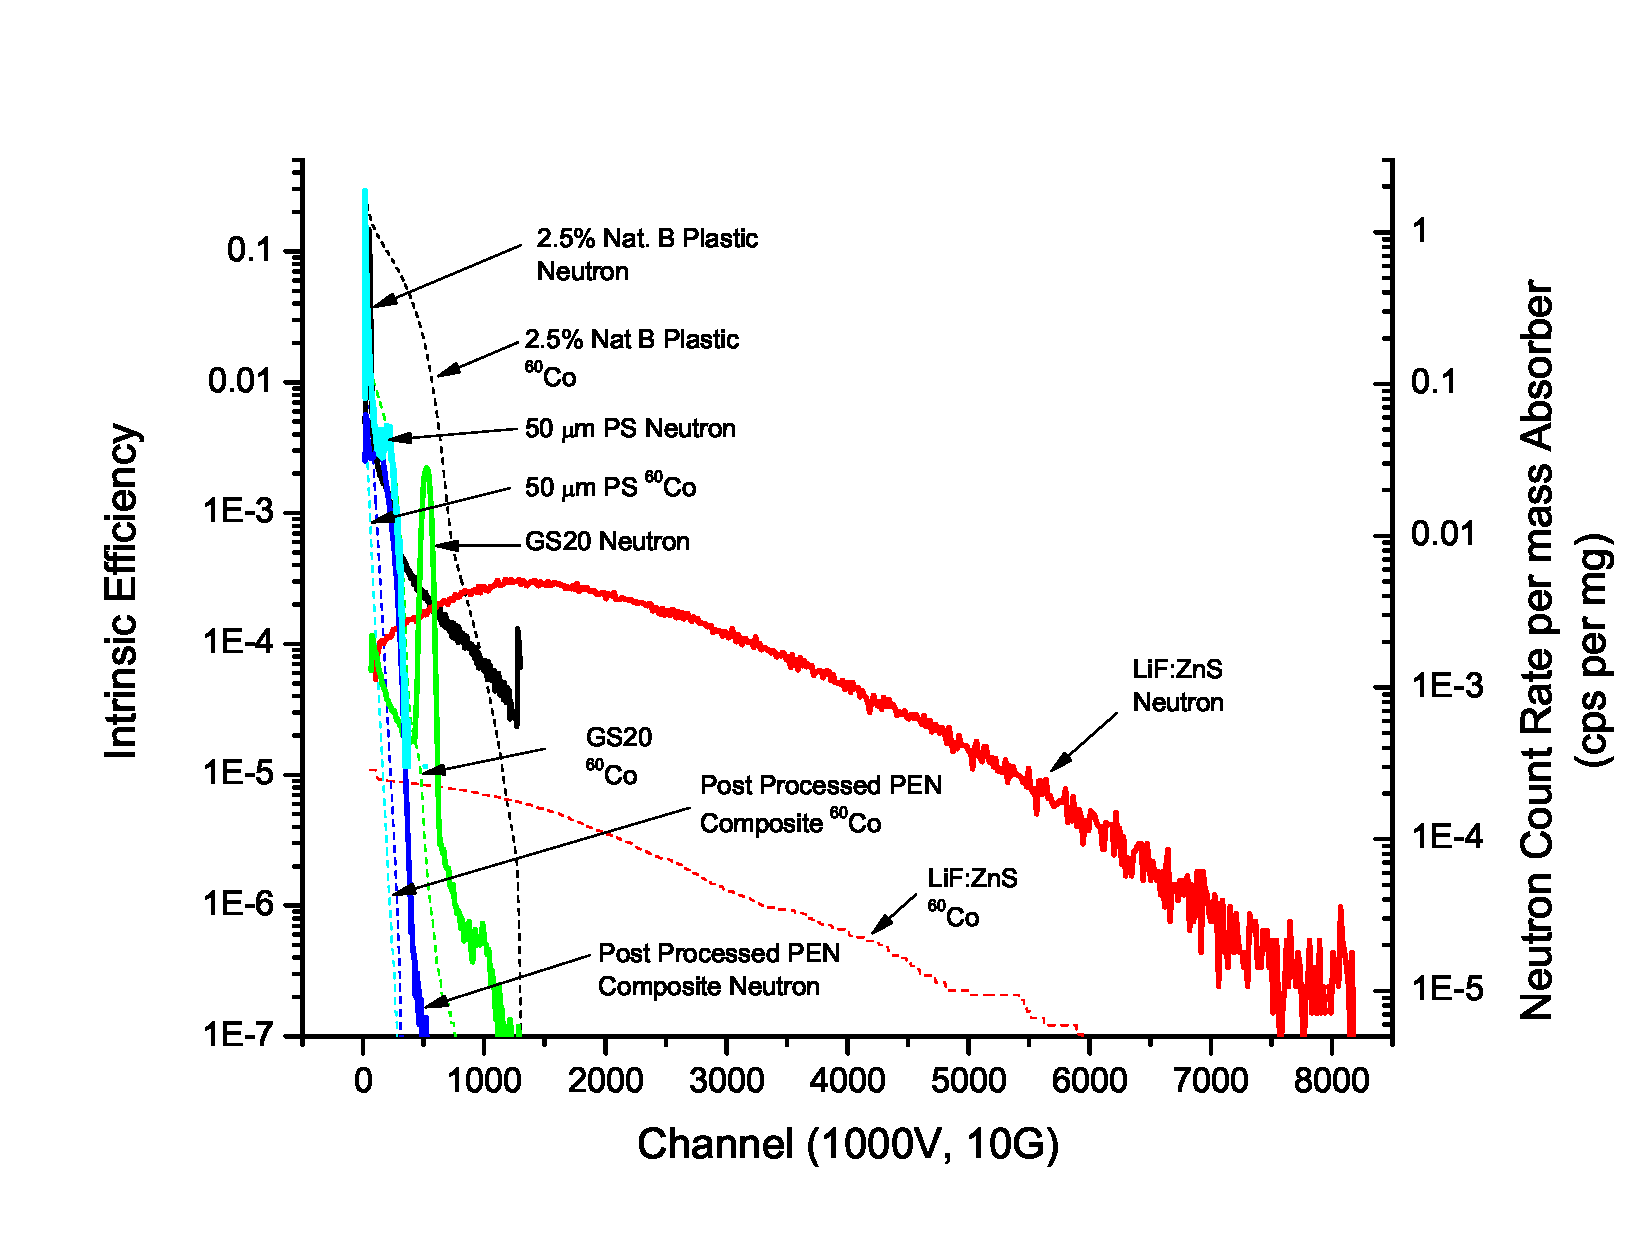
\includegraphics[width=\textwidth]{SampleComparison_IntEff_CR}
  \caption[Gamma Sensitivity and Neutron Response of Measured Detectors]{Gamma sensitivity (left axis, dashed lines) and neutron performance (right axis, solid lines) of measured detectors.  The neutron count rate above the gamma pulse height discriminator may be found by noting where the intrinsic efficiency crosses \num{1E-6} and then integrating the neutron spectra above it. The neutron spectra are from the lead well, and are normalized by the mass of absorber.}
  \label{fig:DiscrimPerformance}
\end{figure}
\autoref{fig:UTDetectorPreformance} demonstrates the performance of two detectors fabricated at UT (the PEN by Rohit Uppal and the PS by Andrew Mabe).
\begin{figure}
  \centering
  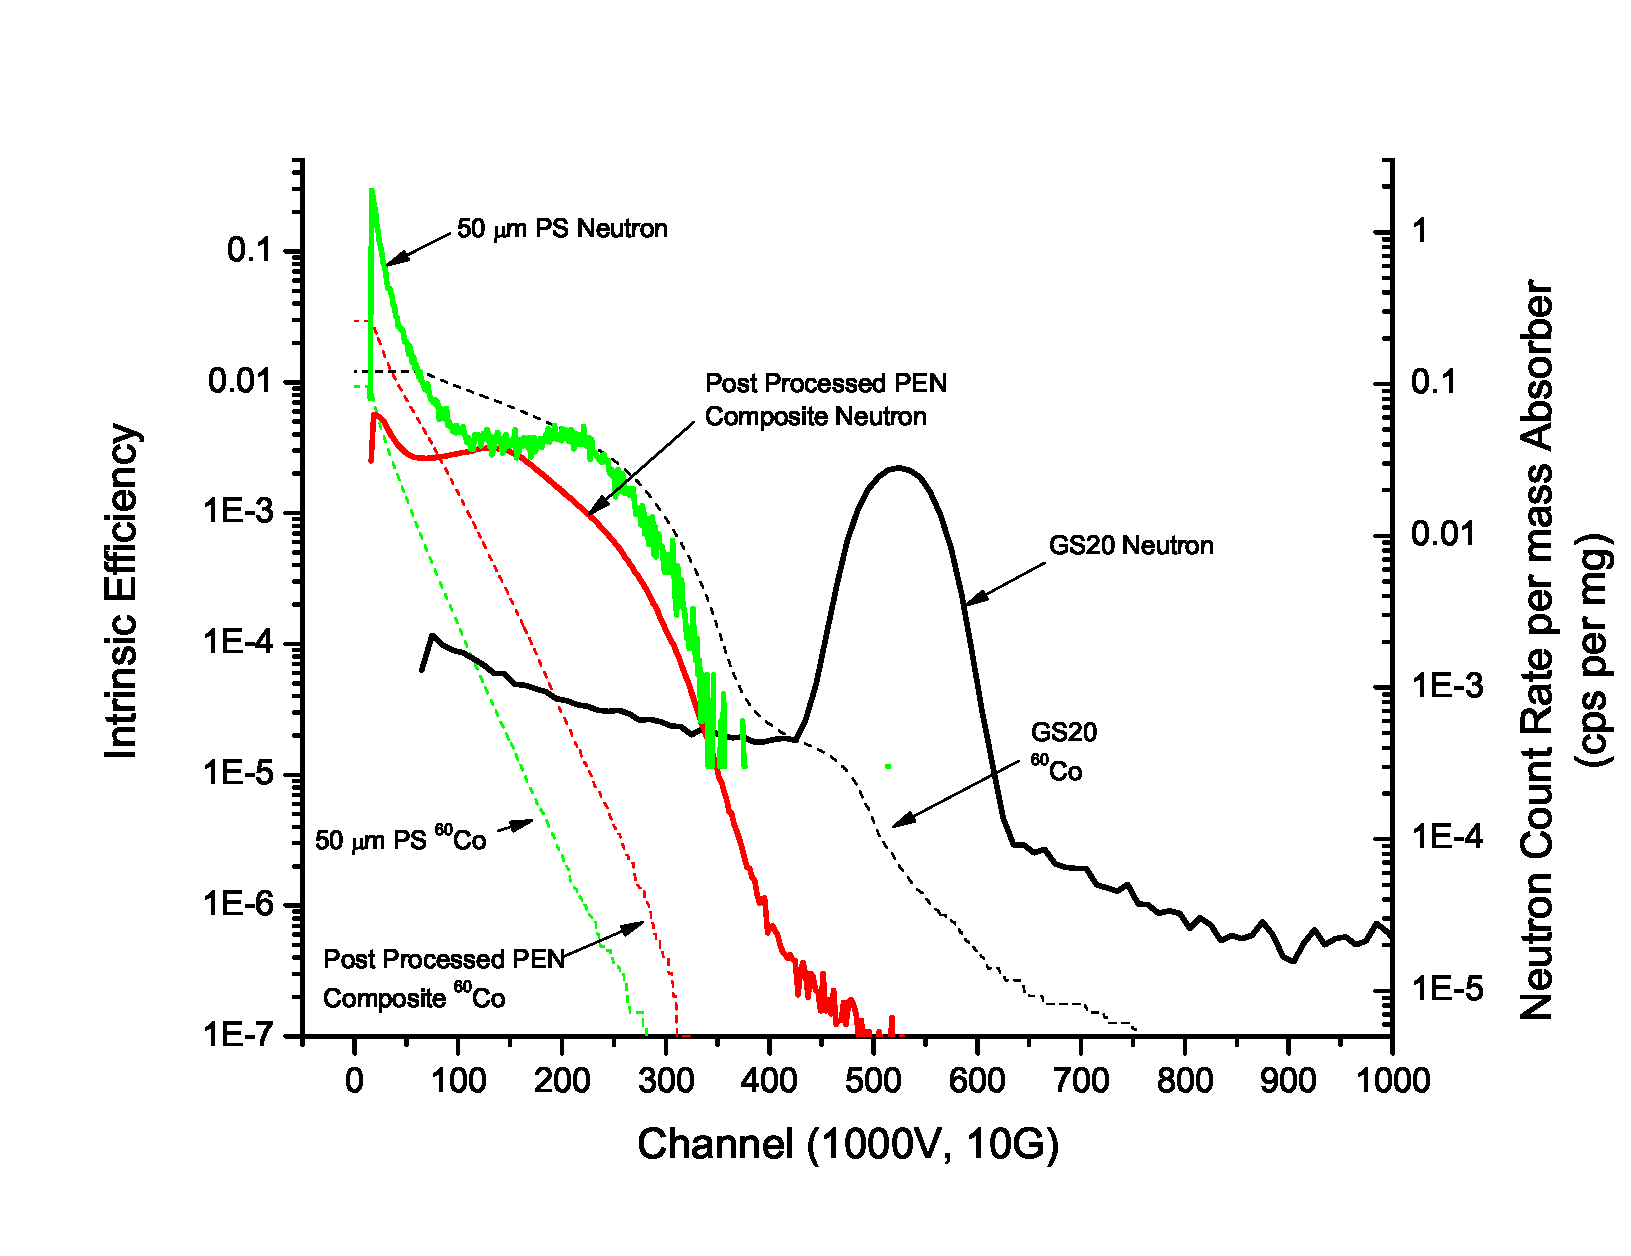
\includegraphics[width=\textwidth]{SC_UTDetectors_IntEff_CR}
  \caption[UT Fabricated Detector Performance]{Performance of a polystyrene and PEN film fabricated at UT compared to GS20.}
  \label{fig:UTDetectorPreformance}
\end{figure}

\subsection{Individual Detector Performance}
The performance of the individual detectors are shown in the separate figures to clearly illustrate important features.
\begin{figure}
  \centering
  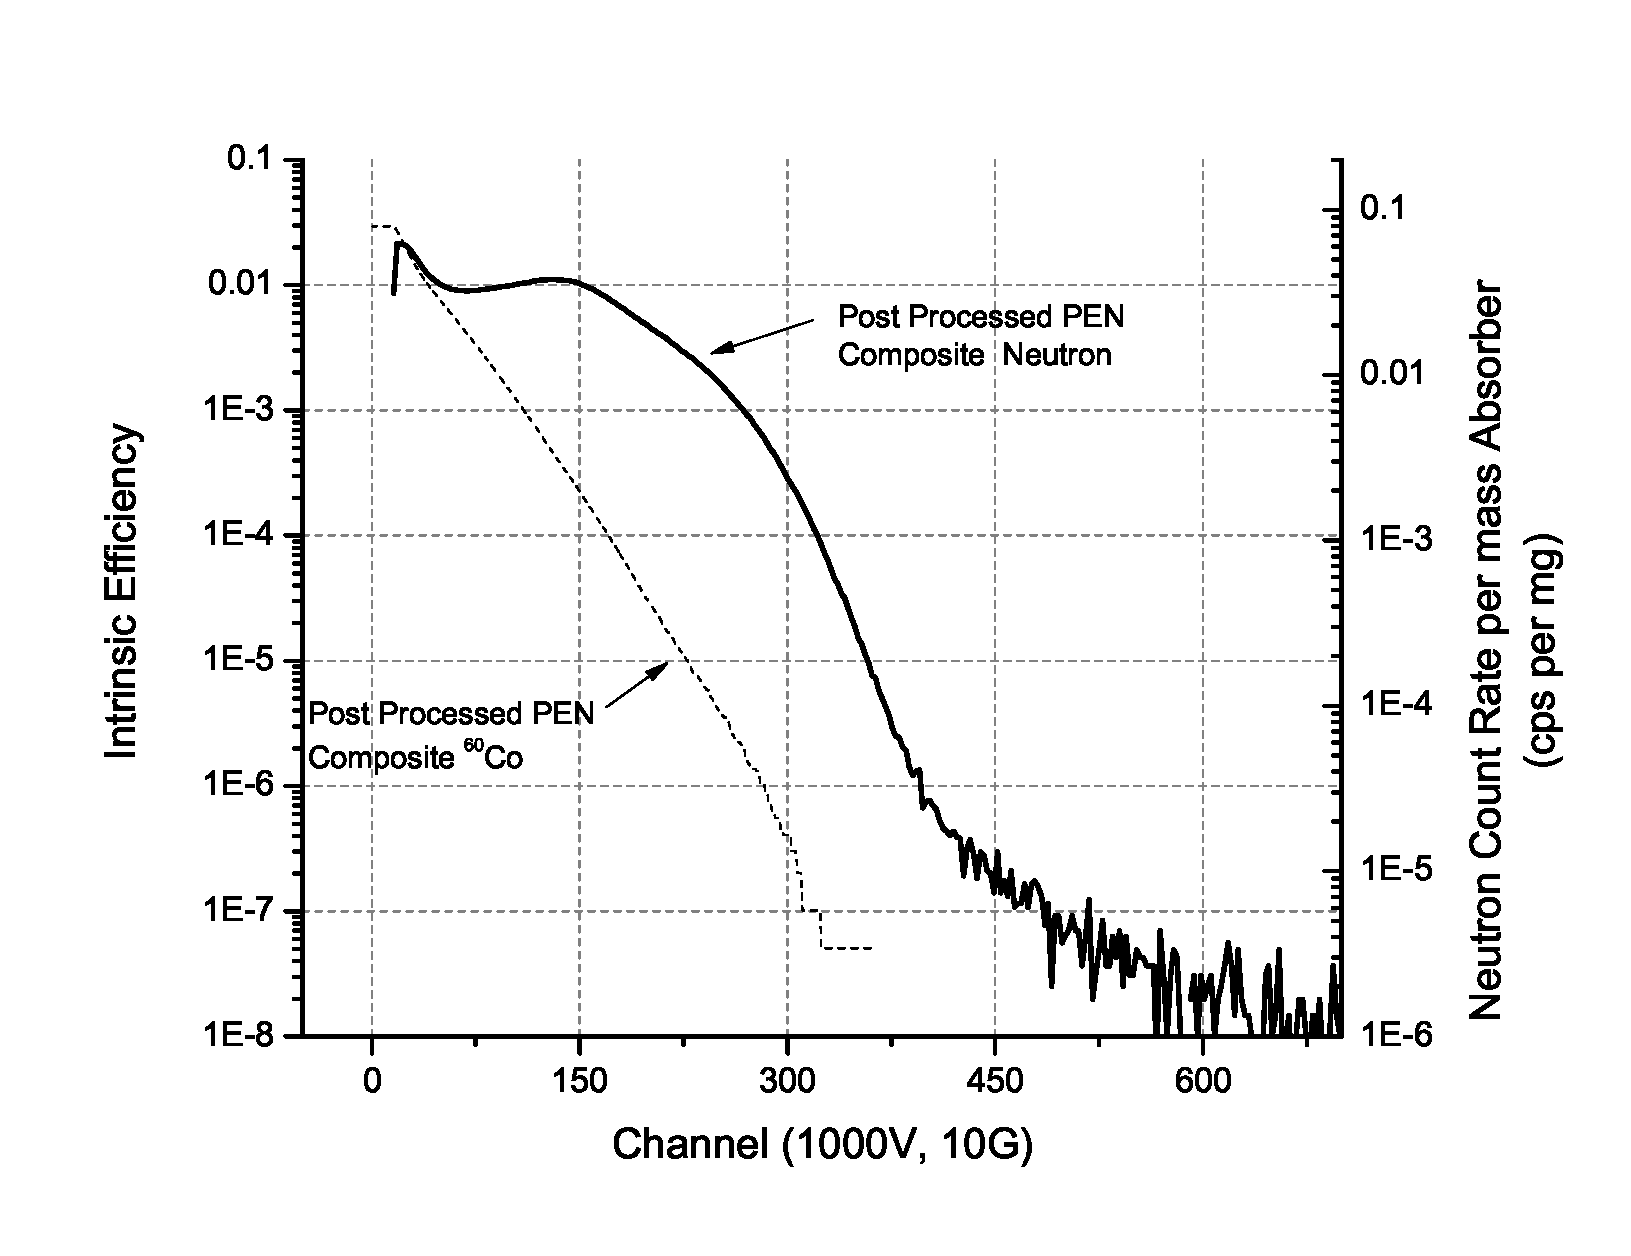
\includegraphics[width=\textwidth]{SC_ACPEN_IntEff_CR}
  \caption[Post processed Composite PEN Performance]{Performance of an Post processed Composite PEN Film (22 March Sample).}
  \label{fig:ACPENPreformance}
\end{figure}
\begin{figure}
  \centering
  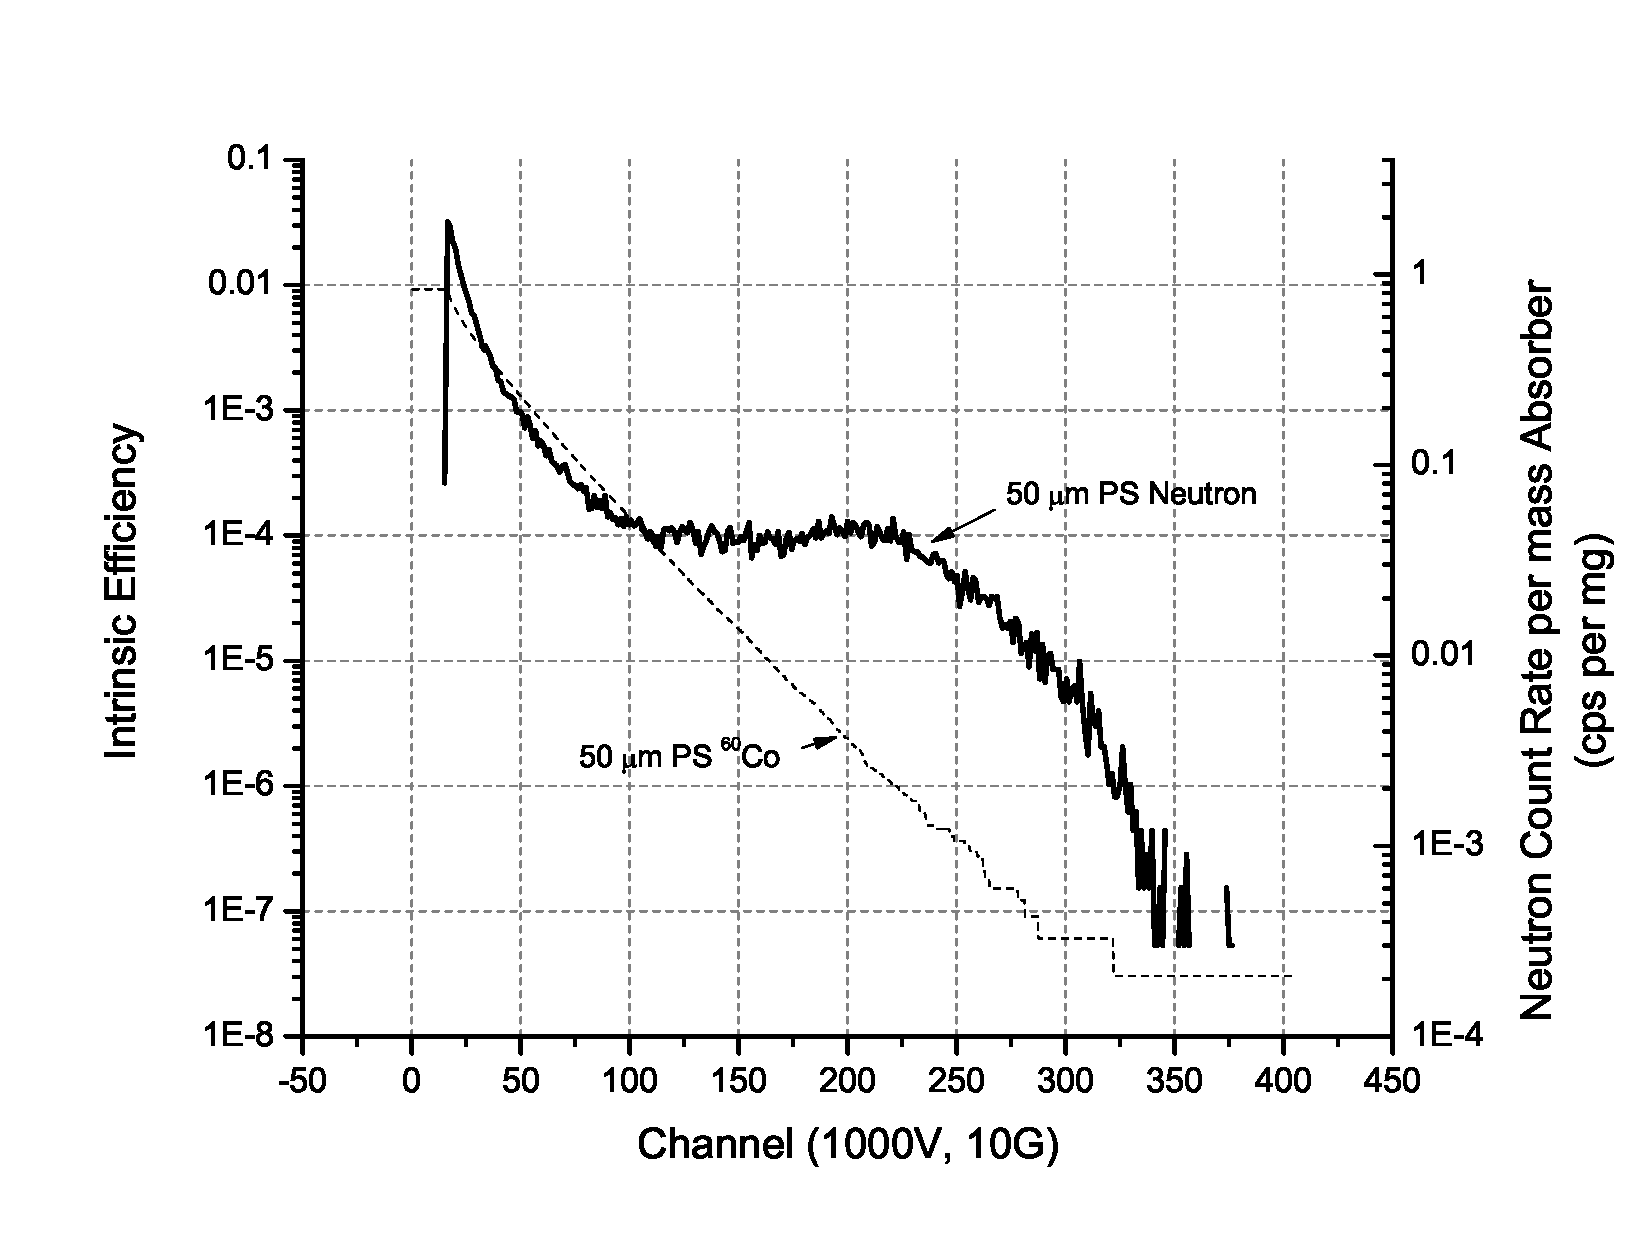
\includegraphics[width=\textwidth]{SC_PS_IntEff_CR}
  \caption[Cast Polystyrene Performance]{Performance of an \SI{50}{\um}, 10\% \iso[6]{LiF} PS Film (24 Jan 2012 Sample).}
  \label{fig:PSPreformance}
\end{figure}
\begin{figure}
  \centering
  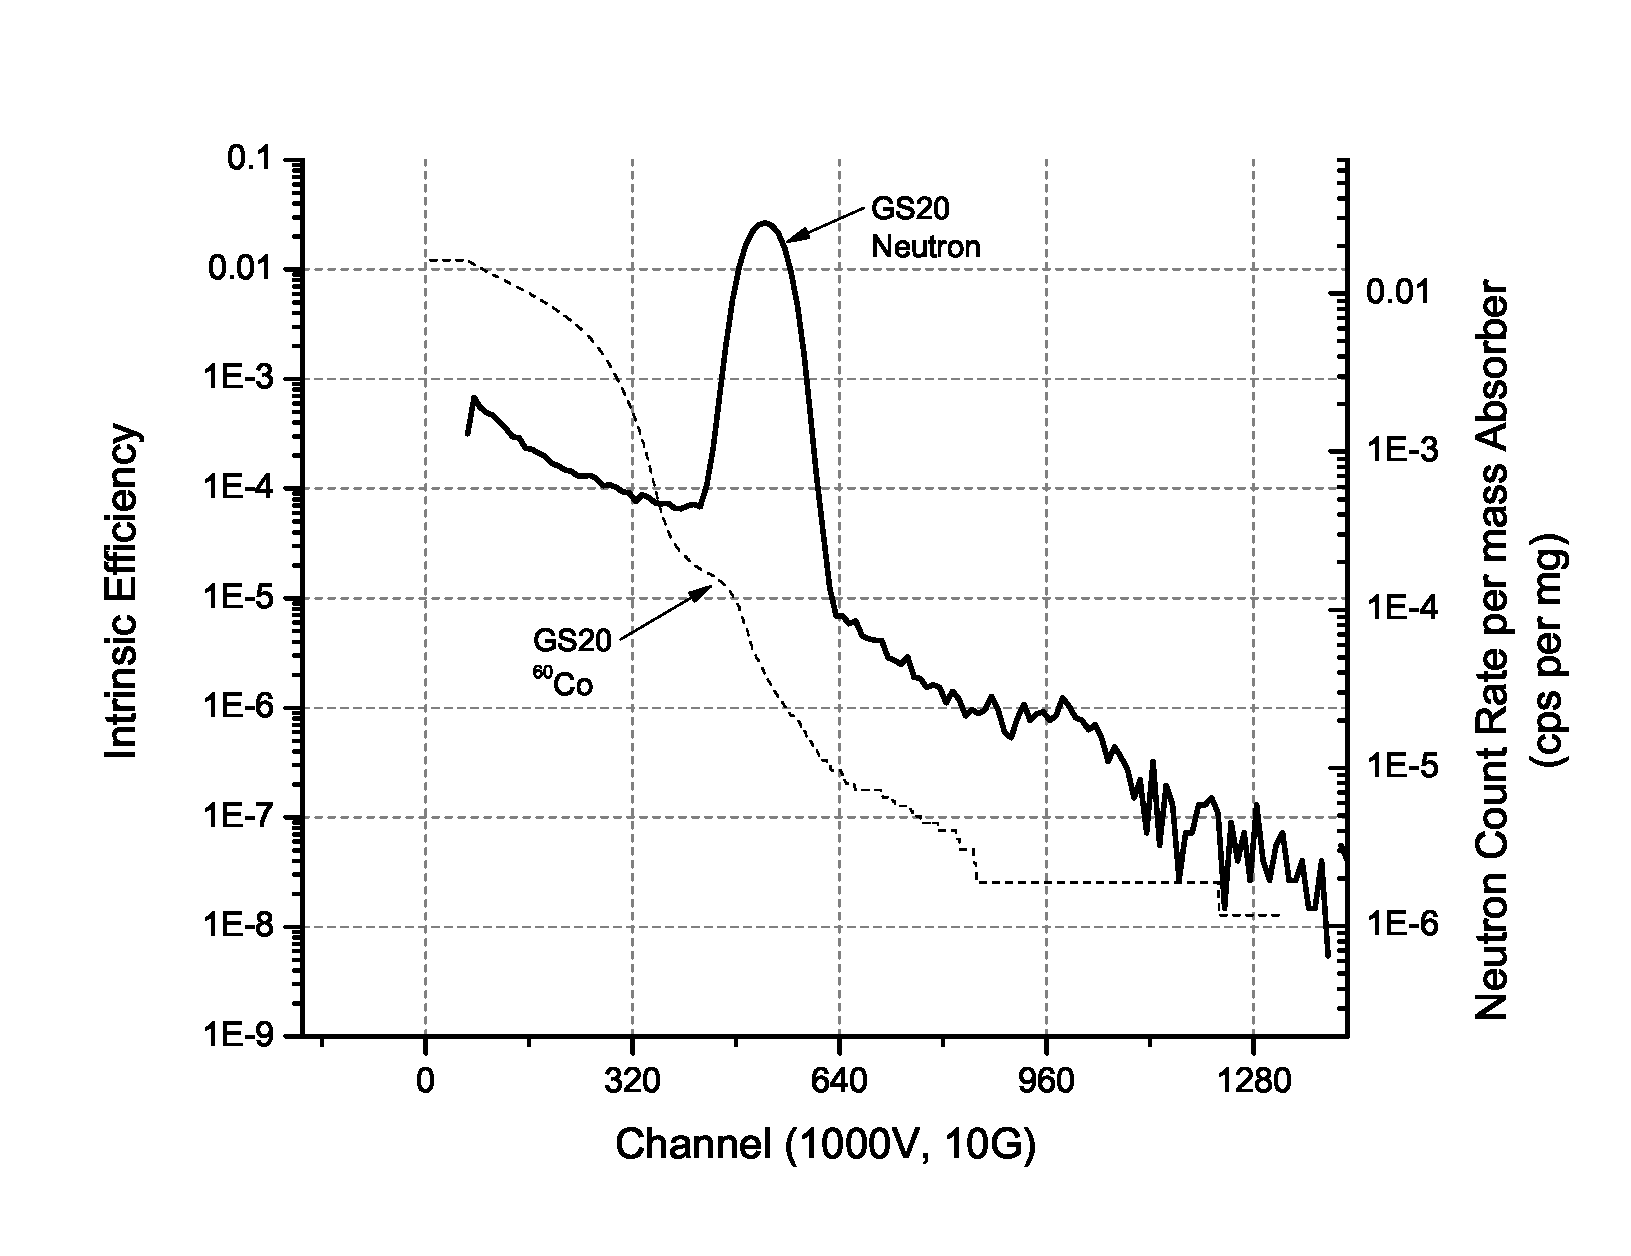
\includegraphics[width=\textwidth]{SC_GS20_IntEff_CR}
  \caption[GS20 Performance]{Performance of \SI{2}{\mm} GS20.  It should be noted that there is significant self shielding in GS20, and that due to the gamma sensitivity catching the tail of the neutron peak the count rate above the gamma pulse height discriminator has the most variation of the samples measured.}
  \label{fig:GS20Preformance}
\end{figure}
\begin{figure}
  \centering
  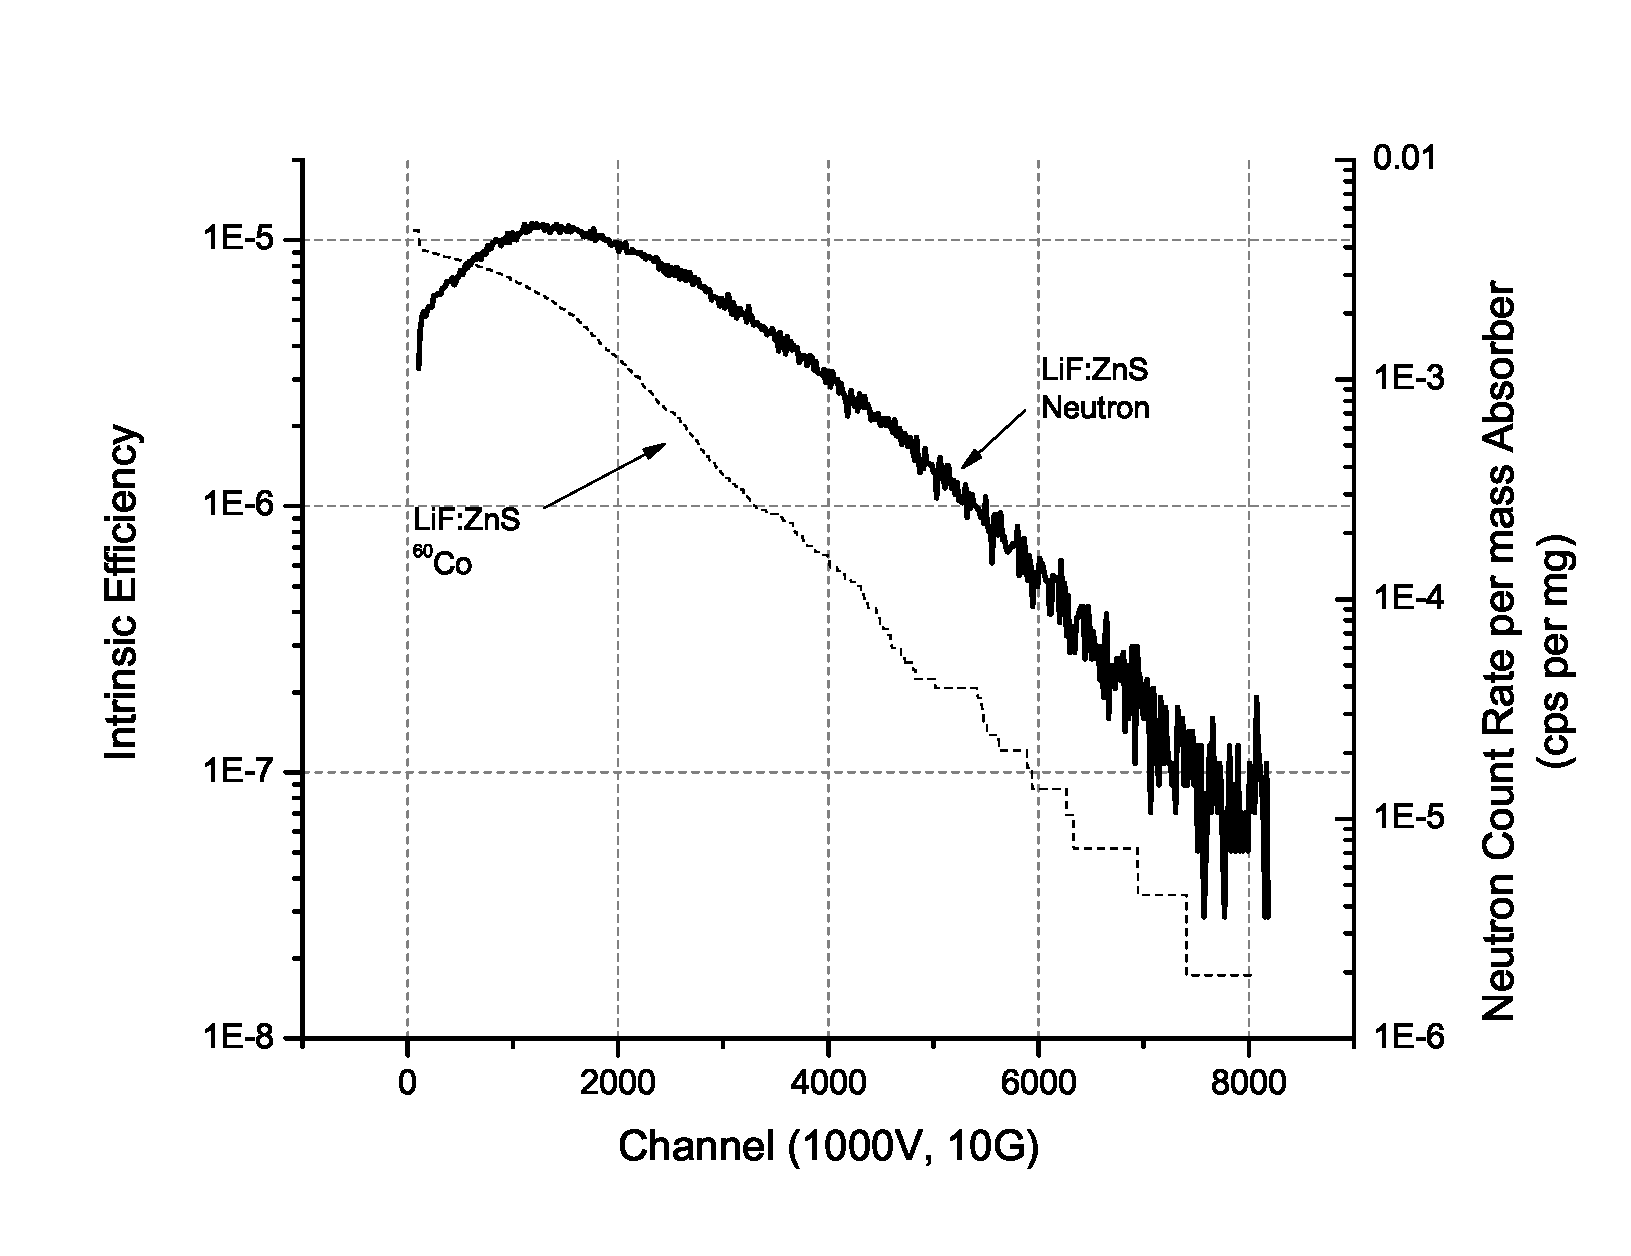
\includegraphics[width=\textwidth]{SC_EJ426_IntEff_CR}
  \caption[EJ 426 Performance]{Performance of EJ-426 HD2 (LiF:ZnS(Ag)) sheet.  This is the brightest scintillator tested, with the lowest gamma sensitivity.}
  \label{fig:EJ254Perf}
\end{figure}
\begin{figure}
  \centering
  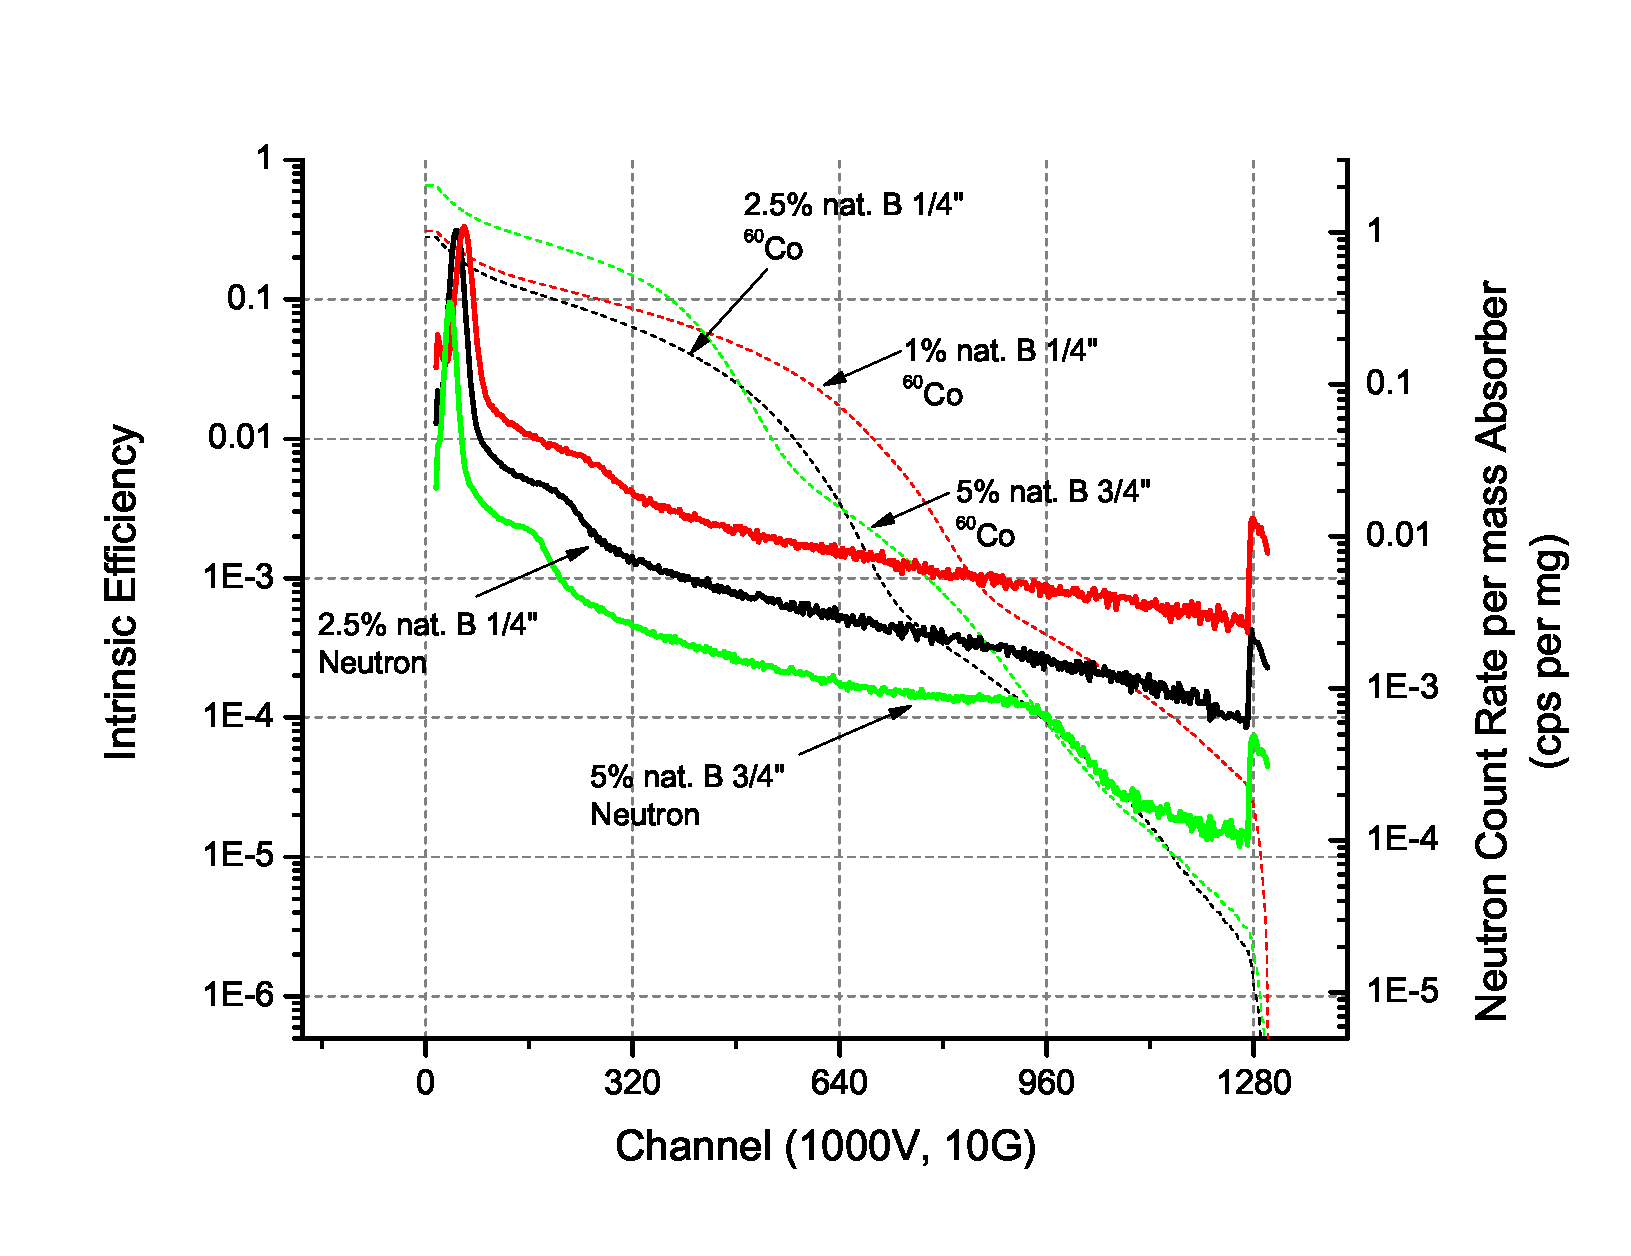
\includegraphics[width=\textwidth]{SC_EJ254_IntEff_CR}
  \caption[EJ 254 Performance]{Performance of EJ-254}
  \label{fig:EJ254Preformance}
\end{figure}
It is apparent that the EJ-254 is not a suitable candidate for replacement detector material in an RPM using a pulse height discriminator.
The reasons for this are twofold: 1) the detector is very thick which increases the probability of a gamma interaction as well as the probability that the interaction will deposit a majority of its energy and 2) \iso[10]{B} has a much lower Q-value (\SI{2.78}{\MeV} compared to \SI{4.78}{\MeV}) and a large pulse height deficit.
However, the material is optically transparent and due to \iso[10]{B}'s large thermal perhaps a thin sheet of EJ-254 might make a suitable detector material.


    %%%%%%%%%%%%%%%%%%%%%%%%%%%%%%%%%%%%%%%%%%%%%%%%%%%%%%%%%%%%%%%%%%%%%%%%%%%
    % A VITA IS REQUIRED
    %%%%%%%%%%%%%%%%%%%%%%%%%%%%%%%%%%%%%%%%%%%%%%%%%%%%%%%%%%%%%%%%%%%%%%%%%%%
    \addToTOC{Vita}
    \chapter*{Vita} \label{ch:vita}
Matthew J. Urffer was born January, 29, 1988 on a small turkey farm on Urffer Road in Coopersburg, Pa.
He got his B.S. in physics from Carnegie Mellon University in Pittsburgh, PA. 
Upon graduation Matthew enrolled at the University of Tennessee, Knoxville where he received his Masters in Nuclear Engineering in December, 2012 and his doctorate in nuclear engineering in December, 2013.

\end{document}
